%\documentclass[12pt,letterpaper,twoside,onecolumn,portrait,leqno]{book}  %leqno= Left numbering for equations
%\documentclass[12pt,letterpaper,twoside,onecolumn,portrait]{book} 
\documentclass[12pt,letterpaper,oneside,onecolumn,portrait]{book} %Kemelli, 3/7/13: to remove bindingoffset
\bibliographystyle{plain}
\usepackage[Sonny]{fncychap} %Bjornstrup, Sonny
\usepackage{amssymb,amsfonts,amsmath,amscd,amsthm}
%\usepackage[draft]{graphicx}
\usepackage{graphicx}
\usepackage[dvips]{epsfig}
\usepackage{rotating}
\usepackage{color}
\usepackage{url}
\usepackage{fancyvrb}
\usepackage{subfig}
\usepackage{wrapfig} 
\usepackage{framed}    % left bar at the left of the new text added 
\usepackage{booktabs}  %nice tables
\usepackage{array} %set fixed length in table columns
\usepackage{textcomp} %textangle
\usepackage{geometry}
\geometry{top=1.00in, bottom=1.00in, left=1.00in, right=1.00in}
\usepackage{enumerate}
\usepackage[algoruled,vlined,linesnumbered,english]{algorithm2e}
\SetAlFnt{\footnotesize}

\usepackage{titlesec} 
\titleformat{\section}{\LARGE\sffamily}{\thesection}{1em}{}
\titleformat{\subsection}{\Large\sffamily}{\thesubsection}{1em}{}
\titleformat{\subsubsection}{\large\sffamily}{\thesubsubsection}{1em}{}
% \usepackage{sectsty}
% \sectionfont{\sffamily}

% Sonny
 %\ChNameVar{\Huge\sf}
% \ChRuleWidth{0.5pt}
% \ChNumVar{\Huge}
% \ChNameUpperCase
 \ChTitleVar{\huge\sf}


\usepackage{hyperref}                       %%% cria links no arquivo .pdf
\hypersetup{colorlinks=true,linkcolor=blue,citecolor=blue}
%\hypersetup{colorlinks=false,linkcolor=blue,citecolor=blue}
                                            %%% comentar as linhas na vers�o para impressao

                                            %%% propriedades do arquivo .pdf

%\hyphenation{es-ta-be-le-ci-das a-tu-al-men-te}

\hypersetup{
   pdftitle = {QUESO user's manual},
   pdfsubject = {The QUESO Library -- Quantification of Uncertainty for Estimation, Simulation, and Optimization},
   pdfkeywords = {research, uncertainty quantification, statistical inverse and statistical forward problems, validation.},
   pdfauthor = {Kemelli C. Estacio-Hiroms}
   }


\setcounter{secnumdepth}{4}                 %%% Habilita 4 n�vel de numera��o
\setlength{\textwidth}{6.6in}
\setlength{\topmargin}{-0.25in}
\setlength{\textheight}{8.60in}
\setlength{\oddsidemargin}{0.2in}
\setlength{\evensidemargin}{-0.3in}

% \renewcommand{\contentsname}{\vspace*{-1.45in}\centerline{\Large\bf Contents}\vspace*{-0.4in}}
% \renewcommand{\listtablename}{\vspace*{-1.45in}\centerline{\Large\bf List of Tables}\vspace*{-0.4in}}
% \renewcommand{\listfigurename}{\vspace*{-1.45in}\centerline{\Large\bf List of Figures}\vspace*{-0.4in}}
% \renewcommand{\chaptername}{\vspace*{-1.45in}{\Huge\bf Chapter}}
% \renewcommand{\appendixname}{\vspace*{-1.45in}{\Huge\bf Appendix}}
% \renewcommand{\bibname}{\vspace*{-1.0in}{\Huge\bf Bibliography}}

\newcommand{\Quesoweb}{\url{https://github.com/libqueso}}
\newcommand{\Queso}{QUESO}
\newcommand{\todo}[1]{ {\color{red} To do: #1} }
\newcommand{\bv}[1]{\ensuremath{\mbox{\boldmath$ #1 $}}}
\newcommand{\post}{\text{posterior}}
\newcommand{\prior}{\text{prior}}
\newcommand{\D}{ {\bf D}}

\newcommand{\myverb}[1]{ \indent{ \begin{verbatim} #1 \end{verbatim} } }
\newcommand{\QUESOversion}{0.50.0}

\usepackage{color}
\definecolor{dkgreen}{rgb}{0,0.6,0}
\definecolor{gray}{rgb}{0.5,0.5,0.5}
\definecolor{mauve}{rgb}{0.58,0,0.82}

\usepackage{listings} % to include codes using \lstinputlisting
\lstset{ %
language=sh,                      % choose the language of the code
basicstyle=\scriptsize\ttfamily,       % the size of the fonts that are used for the code
%stringstyle=\ttfamily,
%commentstyle=\scriptsize\sffamily,
%keywordstyle=\bfseries,        % so funciona com basicstyle=\footnotesize,\ttfamily se eu adicionar \usepackage{bold-extra}
keywordstyle=\color{blue},          % keyword style
commentstyle=\color{dkgreen}\sffamily,       % comment style
stringstyle=\color{mauve},  
identifierstyle=\bfseries,
numberbychapter= true,
numberfirstline=false,
% numbers=left,                   % where to put the line-numbers
numberstyle=\footnotesize,      % the size of the fonts that are used for the line-numbers
stepnumber=5,                   % the step between two line-numbers. If it is 1 each line will be numbered
numbersep=8pt,                  % how far the line-numbers are from the code
%backgroundcolor=\color{white},  % choose the background color. You must add \usepackage{color}
showspaces=false,               % show spaces adding particular underscores
showstringspaces=false,         % underline spaces within strings
showtabs=false,                 % show tabs within strings adding particular underscores
%frameround=fttt,                 % roundish frame - Kemelli
%frame=trBL,          			% single % adds a frame around the code
% frameshape={RYRYYY}{yn}{ny}{RYRYYY},
frameshape={YYYYYY}{yn}{ny}{YYYYYY},
% frameshape={RYRYYY}{ny}{yn}{RYRYYY},
%frame=shadowbox, rulesepcolor=\color{black},
tabsize=2,         				% sets default tabsize to 2 spaces
captionpos=b,           		% sets the caption-position to bottom
breaklines=true,       			% sets automatic line breaking
breakatwhitespace=false,    % sets if automatic breaks should only happen at whitespace
escapeinside={\%*}{*)},         % if you want to add a comment within your code
morekeywords ={rm,ls},
belowskip = 10pt, %\medskipamount%\smallskipamount,
aboveskip =10pt,
}  

\newcommand{\chainsizeresults}{20000}
%\newcommand{\new}[1]{{\marginpar{\color{red}\small\raggedright\textsf{\hspace{0pt} NEW}}} \textbf{#1}}

%\newcommand{\new}[1]{{\marginpar{\color{red}\small\raggedright\textsf{\hspace{0pt} NEW}}} #1}


%\newcommand{\new}[1]{\reversemarginpar{\color{red}\tiny\raggedright\textsf{\hspace{-30pt}\vspace{-25pt} NEW}} \begin{leftbar} #1 \end{leftbar}}
\newcommand{\new}[1]{#1}

\begin{document}

\setlength{\unitlength}{1.0in}
%\setlength{\parindent}{0cm}
%\setlength{\parskip}{2ex}
\pagestyle{headings}
\markright{}
\pagenumbering{roman}
\numberwithin{equation}{section}
\numberwithin{figure}{section}
\numberwithin{table}{section}

 	%------------------------------------------------------------------
\thispagestyle{empty}
{\setlength{\parindent}{0cm}\bf{The QUESO Library}}\hfill $~$\\
\begin{picture}(8,0.1)
\linethickness{3pt}
\put(0,0.1){\line(1,0){6.6}}
\end{picture}
$~$\hfill User's Manual\\
$~$\hfill Version 0.4.0\\
$~$\hfill July 14, 2009\\

\vfill
$~$\\
\begin{center}
{\large\bf Quantification of Uncertainty for Estimation,}\\
{\large\bf Simulation, and Optimization (QUESO)}\\
\end{center}
$~$\\

%\vfill
%$~$\\
%{\bf TERMINOLOGY USED IN THIS MANUAL IS SUBJECT TO CHANGE}

\vfill
$~$\\
{\bf Lead Developer:}\hfill \\
$~\hspace{10pt}$ {\em{Ernesto E. Prudencio}}\hfill\\ 
$~$\\
{\bf Contributors:}\hfill \\
$~\hspace{10pt}$ {\em{Todd A. Oliver}} \hfill \\  %\hfill\\
$~\hspace{10pt}$ {\em{Karl W. Schulz}} \hfill \\

Center for Predictive Engineering and Computational Sciences (PECOS) \hfill\\
Institute for Computational and Engineering Sciences (ICES) \hfill\\
The University of Texas at Austin\hfill\\

\vfill
$~$\\
\begin{picture}(8,0.1)
\linethickness{1.5pt}
\put(0,0.1){\line(1,0){6.6}}
\end{picture}

\clearpage
%------------------------------------------------------------------
\thispagestyle{empty}
$~$\\
\vfill
Copyright \copyright\ 2008-2009 The PECOS Development Team, \texttt{http://pecos.ices.utexas.edu}\\
Permission is granted to copy, distribute and/or modify this document under the terms of
the GNU Free Documentation License, Version 1.2 or any later version published by the Free
Software Foundation; with the Invariant Sections being ``GNU General Public License'' and
``Free Software Needs Free Documentation'', the Front-Cover text being ``A GNU Manual'',
and with the Back-Cover text being ``You have the freedom to copy and modify this GNU Manual''.
A copy of the license is included in the section entitled ``GNU Free Documentation License''.

\clearpage
%------------------------------------------------------------------
\addcontentsline{toc}{chapter}{Abstract}
%\thispagestyle{empty}
\centerline{\Large\bf Abstract}
$~$\\
QUESO is a collection of algorithms and C++ classes aimed for
research in uncertainty quantification,
including
the solution of statistical inverse and statistical forward problems,
the validation of mathematical models under uncertainty and
the prediction of quantities of interest from such models along with
the quantification of their uncertainties.

QUESO is designed for flexibility, portability, easiness of use and
easiness of extension. Its software design follows an object-oriented
approach and its code is written on C++ and over MPI. It can run over
uniprocessor or multiprocessor environments.

QUESO contains two forms of documentation:
a User's Manual available in pdf format
and
a lower-level code documentation available in web based/html format.

This is the User's Manual.
It gives an overview of the QUESO capabilities,
provides procedures for software execution, and includes example studies.

\clearpage
%------------------------------------------------------------------
$~$\\

\clearpage
%------------------------------------------------------------------
\addcontentsline{toc}{chapter}{Disclaimer}
%\thispagestyle{empty}
\centerline{\Large\bf Disclaimer (To be checked by Karl)}
$~$\\
    THIS DOCUMENT WAS PREPARED
    BY THE UNIVERSITY OF TEXAS AT AUSTIN.
    NEITHER THE UNIVERSITY OF TEXAS
    AT AUSTIN, NOR ANY OF ITS INSTITUTES, DEPARTMENTS AND EMPLOYEES, MAKES ANY WARRANTY, EXPRESS OR IMPLIED,
    OR ASSUMES ANY LEGAL LIABILITY OR RESPONSIBILITY FOR THE ACCURACY, COMPLETENESS, OR
    USEFULNESS OF ANY INFORMATION, APPARATUS, PRODUCT, OR PROCESS DISCLOSED, OR REPRESENTS
    THAT ITS USE WOULD NOT INFRINGE PRIVATELY OWNED RIGHTS. REFERENCE HEREIN TO ANY SPECIFIC
    COMMERCIAL PRODUCT, PROCESS, OR SERVICE BY TRADE NAME, TRADEMARK, MANUFACTURER, OR OTHERWISE,
    DOES NOT NECESSARILY CONSTITUTE OR IMPLY ITS ENDORSEMENT, RECOMMENDATION, OR FAVORING BY
    THE UNIVERSITY OF TEXAS AT AUSTIN OR ANY OF ITS INSTITUTES, DEPARTMENTS AND EMPLOYEES THEREOF.
    THE VIEW AND OPINIONS EXPRESSED HEREIN DO NOT NECESSARILY STATE OR REFLECT
    THOSE OF THE UNIVERSITY OF TEXAS AT AUSTIN OR ANY INSTITUTE OR DEPARTMENT
    THEREOF.

\clearpage
%------------------------------------------------------------------
$~$\\

\clearpage
%------------------------------------------------------------------
{\markboth{}{}
\addtocontents{toc}{\protect\markboth{}{}}
}
%\addtocontents{toc}{\protect\thispagestyle{headings}}
\tableofcontents

%\clearpage
%%------------------------------------------------------------------
%$~$\\

\clearpage
%------------------------------------------------------------------
\addcontentsline{toc}{chapter}{Preface}
\thispagestyle{empty}
\centerline{\Large\bf Preface}
$~$\\
The QUESO project started in 2008 as part
of the efforts of the recently established Center for Predictive Engineering and Computational Sciences (PECOS)
at the Institute for Computational and Engineering Sciences (ICES) at The University of Texas at Austin.

The PECOS Center was selected by the National Nuclear Security Administration (NNSA) as one of its new five centers of excellence
under the Predictive Science Academic Alliance Program (PSAAP).
The goal of the PECOS Center is
to advance predictive science and to develop the next generation of advanced computational methods and tools
for the calculation of reliable predictions on the behavior of complex phenomena and systems (multiscale, multidisciplinary).
This objective demands a systematic, comprehensive treatment of the calibration and validation of the mathematical models involved,
as well as the quantification of the uncertainties inherent in such models.
The advancement of predictive science is essential for the application of Computational Science to the solution of realistic problems of national interest.

The QUESO library, since its first version, has been publicly released as open source
under the GNU General Public License and is available for free download world-wide.
See http://www.gnu.org/licenses/gpl.html for more information on the GPL software use agreement.

The QUESO development team currently consists of
Todd A. Oliver,
Ernesto E. Prudencio and
Karl W. Schulz.

{\bf Contact Information:}\\
Ernesto E. Prudencio\\
Institute for Computational and Engineering Sciences\\
1 University Station C0200\\
Austin, Texas 78712

email: prudenci@ices.utexas.edu\\
web: http://pecos.ices.utexas.edu\\
$~$\\

\centerline{\bf Referencing the QUESO Library}

When referencing the QUESO library in a publication, please cite the following:
\begin{verbatim}
@Misc{queso-web-page,
   Author = "Ernesto E. Prudencio and Todd A. Oliver and Karl W. Schulz",
   Title  = "{T}he {QUESO} {L}ibrary: {Q}uantification of {U}ncertainty
             for {E}stimation, {S}imulation and {O}ptimization",
   Note   = "http://pecos.ices.utexas.edu",
   Year   = "2008-2009"}

@TechReport{queso-user-ref,
   Author      = "Ernesto E. Prudencio and Todd A. Oliver and Karl W. Schulz",
   Title       = "{T}he {QUESO} {L}ibrary, {U}ser's {M}anual, {ICES} {T}echnical {R}eport XXYYZZ",
   Institution = "Center for Predictive Engineering and Computational Sciences
                  (PECOS), at the Institute for Computational and Engineering
                  Sciences (ICES), The University of Texas at Austin",
   Year        = "2008-2009"}
\end{verbatim}
$~$\\
$~$\\

\centerline{\bf Acknowledgements}

We would like to thank Sai Hung Cheung, James Martin, Roy Stogner, Rhys Ulerich and
Lucas Wilcox for interesting discussions and constructive feedbacks.

%\clearpage
%%------------------------------------------------------------------
%$~$\\


\pagenumbering{arabic}

% \chapter{Introduction}\label{ch-introduction}
\thispagestyle{headings}
\markboth{Chapter \ref{ch-introduction}: Introduction}{Chapter \ref{ch-introduction}: Introduction}

%The purpose of this chapter is to introduce the main concepts and results necessary for
%a more formal treatment of the prediction problem.
%Section \ref{sc-intro-qoi} presents a first mathematical model of a system, as well as the applicability of Bayes' theorem to our prediction problem.
%The chapter finishes with the presentation of a more detailed model of a system in Section \ref{sc-intro-detail}.

% QUESO stands for Quantification of Uncertainty for Estimation, Simulation and Optimization, and
% it is a library  of statistical algorithms and programming classes for {\it research} on uncertainty quantification (UQ) of mathematical models and their predictions. It has been developed to implement advanced algorithms for Bayesian
% inference, including are many variants of MCMC and the multi-level algorithm.  It is able to handle uni- and multi-processor Linux
% environments and to provide a wide range of diagnostics.

The purpose of this chapter is to introduce relevant terminology, mathematical concepts, and statistical algorithms, together with an overall description of QUESO library.

% It is a parallel object-oriented statistical library dedicated to the research of 
% statistically robust, scalable, load balanced, and fault-tolerant mathematical algorithms for the
% quantification of uncertainty in realistic computational models and predictions related to natural and engineering systems.

\section{Key Statistical Concepts}


Inverse problems are defined as the inverse of direct or forward problems, as the term itself suggests.
Inverse problems apply, in general, to situations were certain quantities of interest are different from the ones that are accessible to measurements \cite{Andersen2001}. 

% A typical feature of inverse problems is that they often fail to fulfill Hadamard's presumptions of well-posedness, i.e., a unique solution may not exist or may not depend continuously  on the given data.
% By reformulating inverse problems for statistical inference,  regularization of ill-posed problems may be obtained through Bayesian approach ( 
% by assuming that the a priori beliefs about the solution before having observed any data can be described by a prior distribution). 

% Statistical inverse theory reformulates inverse problems as problems of statistical inference by means of Bayesian statistics. In Bayesian statistics all quantities are modeled as random variable. The randomness, which reflects the observer's uncertainty concerning their values, is coded in the probability distribution of the quantities. From the perspective of statistical inversion theory, the solution to an inverse problem is the probability distribution of the quantity of interest when all information available has been incorporated in the model. This distribution, called the posterior distribution, describes the degree of confidence about the quantity after the measurement has been performed.

Statistical inverse theory reformulates inverse problems as problems of statistical inference by means of Bayesian statistics: all quantities are modeled as random variables, and probability distribution of the quantities encapsulates the uncertainty observed in their values. The solution to the inverse problem is then the probability distribution of the quantity of interest when all information available has been incorporated in the model. This (posterior) distribution describes the degree of confidence about the quantity after the measurement has been performed \cite{KaSo05}.

Thus, the solution to the statistical inverse problem may be given by Bayes' formula, which express the posterior distribution as a function of the prior distribution and the data represented through the likelihood function.

The likelihood function has an open-form and its evaluation is highly computer intensive.  Moreover, simulation-based posterior inference requires a large number of forward calculations to be performed, therefore, fast and efficient sampling techniques are required for posterior inference.

It is often not straightforward to obtain explicit posterior point estimates of the solution, since it usually involves the evaluation of a high-dimensional integral with respect to a possibly non-smooth posterior distribution. In such cases, an alternative integration technique is the Markov chain Monte Carlo method: posterior means may be estimated using the sample mean from a series of random draws from the posterior distribution.

QUESO is designed in an abstract way so that it can be used by any computational model, as long as a likelihood function (in the case of statistical inverse problems) and a quantity of interest (QoI) function (in the case of statistical forward problems) is provided by the user application.

QUESO library provides tools for both sampling algorithms for statistical inverse problems, following Bayes' formula, and statistical forward problems. It contains Monte Carlo solvers (for autocorrelation, kernel density estimation ans accuracy assessment), MCMC (e.g. Metropolis Hastings \cite{Metr_1953,Hast_1970}) as well as the DRAM \cite{HaLaMiSa06} (for sampling from probability distributions); it also has the capacity to handle many chains or sequences in parallel, each chain or sequence itself demanding many computing nodes because of the computational model being statistically explored \cite{PrSc09}.



A computational model is a combination of a
mathematical model and a discretization that enables the approximate
solution of the mathematical model using computer algorithms and  might be used in two different types of problems:
forward or inverse. 

Any computational model is composed of a vector $\boldsymbol{\theta}$ of $n$ {\it parameters}, {\it state variables} $\mathbf{u}$, and {\it state equations} $\mathbf{r}(\boldsymbol{\theta},\mathbf{u}) = \mathbf{0}$.
Once the solution $\mathbf{u}$ is available, the computational model also includes extra functions for e.g.
the calculation of {\it model output data} $\mathbf{y} = \mathbf{y}(\boldsymbol{\theta},\mathbf{u})$, and the {\it prediction} of a
vector $\mathbf{q} = \mathbf{q}(\boldsymbol{\theta},\mathbf{u})$ of $m$~quantities~of~interest\text{ (QoI)},

Parameters designate all model variables that are neither state variables
nor further quantities computed by the model, such as: material properties, coefficients, constitutive parameters, boundary conditions, initial conditions,
external forces, parameters for modeling the model error, characteristics of an experimental apparatus (collection of devices and procedures),
discretization choices and numerical algorithm options.

% Some parameters might be directly measurable, e.g. room temperature,
% but some may not, e.g. a material property.
% Parameters that cannot be measured directly need to be {\it estimated}
% through the solution of an {\it inverse problem}.


In the case of a forward problem, the parameters $\boldsymbol{\theta}$ are given and
one then needs to compute $\mathbf{u}$, $\mathbf{y}$ and/or $\mathbf{q}$.
In the case of an inverse problem, however, experimental data $\mathbf{d}$ is given and
one then needs to {\it estimate} the values of the parameters $\boldsymbol{\theta}$ that
cause $\mathbf{y}$ to best fit  $\mathbf{d}$.
%where ``best'' is an algorithm dependent concept.

%The process of parameter estimation is also referred to as model calibration or model update, and it usually precedes the computation of a QoI, a process called model prediction. 

Figure~\ref{fig-generic-problems} represents general inverse and forward problems respectively.
%
\begin{figure*}[htb]
\begin{minipage}[b]{0.5\textwidth}
\input{rawfigs/gfp01.latex}\\
\centering
(a)
\end{minipage}%\hfill
\begin{minipage}[b]{0.5\textwidth}
\input{rawfigs/gip01.latex}\\
\centering 
(b)
\end{minipage}
%\end{center}
\vspace{-20pt}
\caption{The representation of (a) a generic forward problem and (b) a generic inverse problem.}
\label{fig-generic-problems}
\end{figure*}


There are many possible sources of uncertainty on a computational model. %procedures (a) and (b) above. 
First, $\mathbf{d}$ need not be equal to the actual values of observables because of errors in the measurement process. Second, the values of the input parameters to the phenomenon might not be precisely known. Third, the appropriate set of
equations governing the phenomenon might not be well understood. 

Computational models can be classified as either deterministic or stochastic -- which are the ones of interest here.  In deterministic models, all parameters are assigned numbers, and no parameter is related to the parametrization of a random variable (RV) or field. As a
consequence, a deterministic model assigns a number to each of the components of quantities $\mathbf{u}$, $\mathbf{y}$ and $\mathbf{q}$. In stochastic models, however, at least one parameter is assigned a probability density function (PDF) or is related to the parametrization of a RV or field, causing $\mathbf{u}$, $\mathbf{y}$ and $\mathbf{q}$ to become random variables.  Note that not all components of $\boldsymbol{\theta}$ need to be treated as random. As long as at least one component is random, $\boldsymbol{\theta}$ is a random vector, and the problem is stochastic.



In the case of forward problems, statistical forward problems can be represented very similarly to deterministic forward problems,
as seen in Figure \ref{fig-sfp-queso}.
In the case of inverse problems, as depicted in Figure \ref{fig-sip-queso}, however, the conceptual connection between deterministic and statistical problems
is not as straightforward.

\begin{figure}[h!]
\centerline{
\input{rawfigs/sfp01.latex}\\
}
\caption{
The representation of a statistical forward problem.
$\boldsymbol{\Theta}$ denotes a random variable related to parameters,
$\boldsymbol{\theta}$ denotes a realization of $\boldsymbol{\Theta}$ and
$\mathbf{Q}$ denotes a random variable related to quantities of interest.
}
\label{fig-sfp-queso}
\end{figure}

\begin{figure}[h!]
\centerline{
\input{rawfigs/sip01.latex}\\
}
\caption{
The representation of a statistical inverse problem.
$\boldsymbol{\Theta}$ denotes a random variable related to parameters,
$\boldsymbol{\theta}$ denotes a realization of $\boldsymbol{\Theta}$ and
$\mathbf{r}$ denotes model equations,
$\mathbf{y}$ denotes some model output data and
$\mathbf{d}$ denotes experimental data.
}
\label{fig-sip-queso}
\end{figure}


QUESO adopts a Bayesian analysis \cite{KaSo05, Ro04} for statistical inverse problems, interpreting the posterior PDF
\begin{equation}\label{eq-Bayes-solution}
\pi_{\text{posterior}}(\boldsymbol{\theta}|\mathbf{d})=\frac{\pi_{\text{prior}}(\boldsymbol{\theta})\pi_{\text{likelihood}}(\mathbf{d}|\boldsymbol{\theta})}{\pi(\mathbf{d})}
\end{equation}
as the solution. Such solutions combine the prior information $\pi_{\text{prior}}(\boldsymbol{\theta})$ of the parameters,
the information $\pi(\mathbf{d})$ on the data, and the likelihood $\pi_{\text{likelihood}}(\mathbf{d}|\boldsymbol{\theta})$ that the model computes certain data values with a given set of input parameters.

This semantic interpretation of achieving a posterior knowledge on the parameters (on the model)
after combining some prior model knowledge with experimental information provides an important mechanism for dealing with uncertainty.
Although mathematically simple, is not computationally trivial. 


\section{The Software Stack of an Application Using QUESO}
%TAKEN FROM QUESO PAPER, SECTION 3

% Section \ref{sc-concepts} identified many mathematical entities present in the description of statistical problems and in some algorithms used for their solution.
% As part of the design, QUESO attempts to conceptually implement these entities in order to allow algorithmic researchers to manipulate
% them at the library level, as well as for algorithm users (the modelers interested in UQ) to manipulate them at the application level.
% Examples of entities are 
% vector space $\mathbb{R}^n$;
% vector subset $B\subset\mathbb{R}^n$;
% vector $\boldsymbol{\theta}\in B$;
% matrix $\mathbf{C}\in \mathbb{R}^n\times\mathbb{R}^n$;
% function $\pi:\mathbb{R}^n\rightarrow\mathbb{R}_+$, e.g. joint PDF;
% function $\pi:\mathbb{R}\rightarrow\mathbb{R}_+$, e.g. marginal PDF;
% function $\pi:\mathbb{R}\rightarrow[0,1]$, e.g. cumulative distribution function;
% realizer function;
% function $\mathbf{q}:\mathbb{R}^n\rightarrow\mathbb{R}^m$;
% sequences of scalars; and
% sequences of vectors.
% QUESO tries to naturally map such entities through an object-oriented design.
% Indeed, QUESO C++ classes include vector spaces, subsets, scalar sequences, PDFs, and RVs.


An application using QUESO falls into three categories: a statistical inverse problem (IP), a statistical forward problem (FP), or combinations of both.
In each problem the user might deal with up to five vectors of potentially very different sizes:
parameters $\boldsymbol{\theta}$, state $\mathbf{u}$, output $\mathbf{y}$, data $\mathbf{d}$ and QoIs $\mathbf{q}$.

Algorithms in the QUESO library require the supply
of a likelihood routine $\pi_{\text{like}}:\mathbb{R}^n\rightarrow\mathbb{R}_+$ for statistical inverse problems and 
of a QoI routine $\mathbf{q}:\mathbb{R}^n\rightarrow\mathbb{R}^m$ for statistical forward problems. These routines
exist at the application level and provide the necessary bridge between the statistical algorithms in QUESO,
model knowledge in the model library and scenario and experimental data in the disk space.
%Concepts are further detailed in Chapter \ref{ch-introduction}.
%
Figure~\ref{fig-sw-stack} shows the software stack of a typical application that uses QUESO. In the figure, the symbol $\boldsymbol{\theta}$ represents a vector of $n\geqslant 1$ parameters. 
%
\begin{figure}[!htbp]
\centerline{
%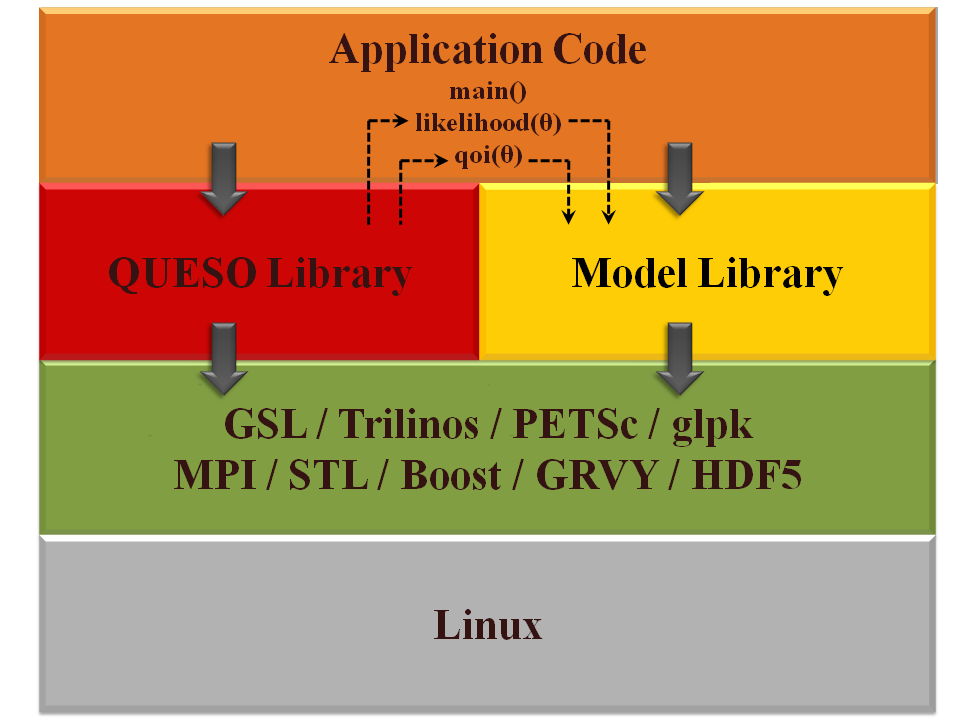
\includegraphics[scale=0.4,clip=true]{rawfigs/quesoSwStack_09_2010.png}
}
\caption{
An application software stack.
QUESO requires the input
%supply
of a likelihood routine $\pi_{\text{like}}:\mathbb{R}^n\rightarrow\mathbb{R}_+$ for IPs and 
of a QoI routine $\mathbf{q}:\mathbb{R}^n\rightarrow\mathbb{R}^m$ for FPs.
These application level routines provide the bridge between
% among
the statistical algorithms in QUESO,
physics 
%model
knowledge in the model library, and relevant 
experimental (calibration
    and validation) data.
%model specific data in the disk space.
}
\label{fig-sw-stack}
\end{figure}

% \begin{figure}[h!]
% \centerline{
% 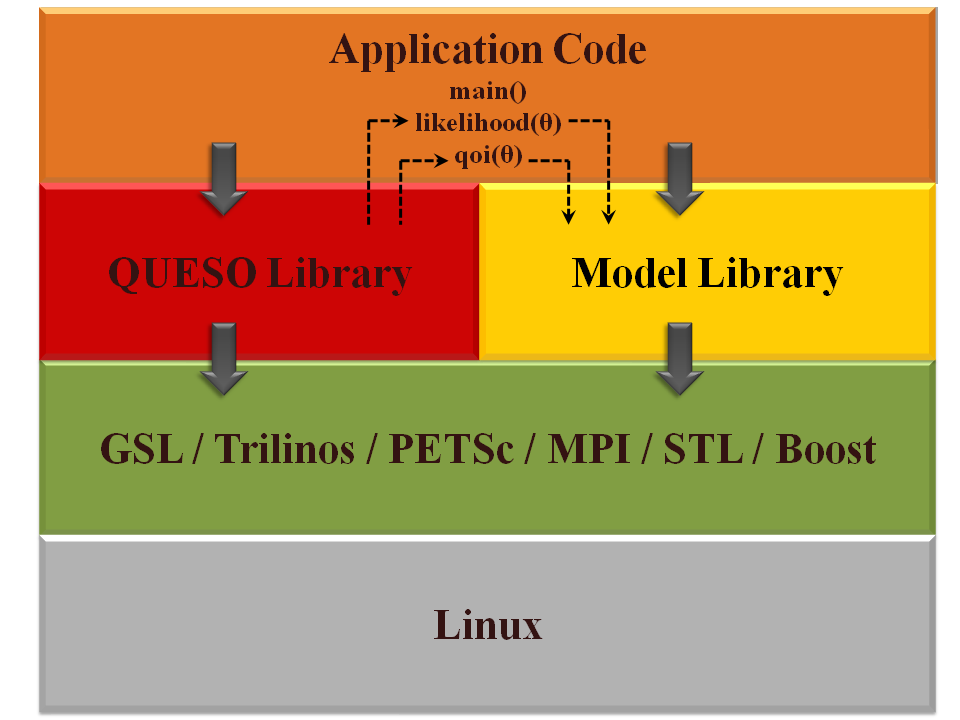
\includegraphics[scale=0.50,clip=true]{figs/queso_paper1_03}
% }
% \caption{
% Overview of the software stack of a typical application that uses QUESO.
% The symbol $\boldsymbol{\theta}$ represents a vector of $n\geqslant 1$ parameters.
% Algorithms in the QUESO library require the supply
% of a likelihood routine $\pi_{\text{like}}:\mathbb{R}^n\rightarrow\mathbb{R}_+$ for statistical inverse problems and 
% of a qoi routine $\mathbf{q}:\mathbb{R}^n\rightarrow\mathbb{R}^m$ for statistical forward problems. These routines
% exist at the application level and provide the necessary bridge between the statistical algorithms in QUESO,
% model knowledge in the model library and scenario and experimental data in the disk space.
% Concepts are further detailed in Chapter \ref{ch-introduction}.
% }
% \label{fig-sw-stack}
% \end{figure}
%
Even though QUESO deals directly with $\boldsymbol{\theta}$ and $\mathbf{q}$ only,
it is usually the case the one of the other three vectors ($\mathbf{u}$, $\mathbf{y}$ and $\mathbf{d}$) will have the biggest number of components and will therefore
dictate the size of the minimum parallel environment to be used in a problem.
%
So, for example, even though one processor might be sufficient for handling $\boldsymbol{\theta}$, $\mathbf{y}$, $\mathbf{d}$ and $\mathbf{q}$,
eight processors at least might be necessary to solve for $\mathbf{u}$.
QUESO currently only requires that the amounts $n$ and $m$ can be handled by the memory available to one processor,
which allows the analysis of problems with thousands of parameters and QoIs, a large amount even for state of the art UQ algorithms.

QUESO currently supports three modes of parallel execution:
an application user may simultaneously run:
\begin{description}
\item[(a)] multiple instances of a problem where the physical model requires a single processor, or
\item[(b)] multiple instances of a problem where the physical model requires multiple processors, or
\item[(c)] independent sets of types (a) and (b).
\end{description}
%
For example, suppose an user wants to use the MH algorithm to solve a statistical IP, and that 1,024 processors are available.
If the physical model is simple enough to be handled efficiently by a single processor, then the user can run 1,024 chains simultaneously, as in case (a).
If the model is more complex and requires, say, 16 processors, then the user can run 64 chains simultaneously, as in case (b), with 16 processors per chain.
QUESO treats this situation by using only 1 of the 16 processors to handle the chain.
When a likelihood evaluation is required, all 16 processors call the likelihood routine simultaneously.
Once the likelihood returns its value, QUESO puts  15 processors into idle state until the routine is called again or the chain completes.
Case (c) is useful, for instance, in the case of a computational procedure involving two models,
where a group of processors can be split into two groups, each handling one model.
Once the two model analysis end, the combined model can use the full set of processors.\footnote{The parallel capabilities of QUESO have been exercised on the Ranger system of the TACC \cite{tacc} with up to 1,024 processors \cite{ChOlPr10}.}




\subsection{A QUESO Environment}

Classes in QUESO can be divided in four main groups:
\begin{description}
 \item[ core:] environment (and options), vector, matrix;
\item[ templated basic:] vector sets (and subsets, vector spaces),  scalar function, vector function, scalar sequence, vector sequence;
%\item Vector sets, subsets and spaces (see Figure \ref{fig-vector-space-subset-classes}),
%\item Scalar function (see Figure \ref{fig-scalar-function-class}),
%\item Vector function (see Figure \ref{fig-vector-function-class}),
%\item Scalar sequence (see Figure \ref{fig-scalar-sequence-class}), and
%\item Vector sequence (see Figure \ref{fig-vector-sequence-class}).
\item[ templated statistical:] vector realizer, vector RV, statistical IP (and options), MH solver (and options), statistical FP (and options), MC solver (and options), sequence statistical options;
%\item Vector RV (concatenation)
%\item Statistical IP (and options)
%\item Metropolis Hastings solver (and options)
%\item Statistical FP (and options)
%\item MC solver (and options)
%\item Sequence statistical options
\item[ miscellaneous:] C and FORTRAN interfaces.
\end{description}


The templated basic classes are necessary for the definition and description of other entities, such as RVs, Bayesian solutions of IPs, sampling algorithms and chains.
%
In the following we briefly explain ten QUESO classes.

\subsubsection{Environment Class}
%
This class sets up the environment underlying the use of the QUESO library by an executable.
The constructor of the environment class requires a communicator, the name of an options input file,
and the eventual prefix of the environment in order for the proper options to be read (multiple environments can coexist, as explained further below).
The environment class:
\begin{itemize}
\item[(a)] assigns rank numbers, other than the world rank, to nodes participating in a parallel job,
\item[(b)] provides MPI communicators for generating a sequence of vectors in a distributed way,
\item[(c)] provides functionality to read options from the options input file (whose name is passed in the constructor of this environment class), and
\item[(d)] opens output files for messages that would otherwise be written to the screen (one output file per allowed rank is opened and allowed ranks can be specified through the options input file).
 
\end{itemize}



Let $S \geqslant 1$ be the number of problems a QUESO environment will be handling at the same time, in parallel.
$S$ has default value of $1$ and is an option read by QUESO from the input file provided by the user.
The QUESO environment class manages five types of communicators, referred to as:
\begin{description}
\item[{\it world} :] MPI\_WORLD\_COMM;
\item[{\it full} :] communicator passed to the environment constructor, of size $F$ and usually equal to the world communicator;
\item[{\it sub} :] communicator of size $F/S$ that contains the number of MPI nodes necessary to solve a statistical IP or a statistical FP;
\item[{\it self} :] MPI\_SELF\_COMM, of size 1; and
\item[{\it inter0} :] communicator of size $S$ formed by all MPI nodes that have subrank 0 in their respective subcommunicators.
\end{description}


A {\it subenvironment} in QUESO is the smallest collection of processors necessary for the proper run of the model code.
An {\it environment} in QUESO is the collection of all subenvironments, if there is more than one subenvironment.
So, for instance, if the model code requires 16 processors to run and the user decides to run 64 Markov chains in parallel,
then the environment will consist of a total of $F=1024$ processors and $S=64$ subenvironments, each subenvironment with $F/S=16$ processors.
Any given computing node in a QUESO run has potentially five different ranks.
Each subenvironment is assigned a subid varying from $0$ (zero) to $S-1$, and is able to handle a statistical IP and/or a statistical FP.
That is, each subenvironment is able to handle a {\it sub} Markov chain (a sequence) of vectors and/or a {\it sub} MC sequence of output vectors.
The {\it sub} sequences form an unified sequence in a distributed way.
QUESO takes care of the unification of results for the application programming and for output files.

\subsubsection{Vector Set Class}
%%\label{subsc-vector-set}
%
The vector set class is fundamental for the proper handling of many mathematical entities.
Indeed, the definition of a scalar function such as $\pi:\mathbf{B}\subset\mathbb{R}^n\rightarrow\mathbb{R}$ requires the
specification of the domain $\mathbf{B}$, which is a {\it subset} of the {\it vector space} $\mathbb{R}^n$, which is itself a {\it set}.
The relationship among the classes set, subset and vector space is sketched in Figure \ref{fig-vector-space-subset-classes}.

An attribute of the {\it subset} class is the {\it vector space} which it belongs to, and in fact a reference to a vector space is required by the constructor of the subset class.
The power of an object-oriented design is clearly featured here.
The {\it intersection} subset derived class is useful for handling a posterior PDF \eqref{eq-Bayes-solution},
since its domain is the intersection of the domain of the prior PDF with the domain of the likelihood function.


\begin{figure}[!h]
\centerline{
\includegraphics[scale=0.35,clip=true]{figs/uqVectorSetConcise}
}
\caption{
The class diagram for vector set, vector subset and vector space classes.
}
\label{fig-vector-space-subset-classes}
\end{figure}

\subsubsection{Scalar Function and Vector Function Classes}
%
PDFs are examples of scalar functions.
QUESO currently supports basic PDFs such as uniform and Gaussian.
See Diagram \ref{fig-scalar-function-class}.
%%The handling of vector functions is as easy.
%%Indeed,
The definition of a vector function $\mathbf{q}:\mathbf{B}\subset\mathbb{R}^n\rightarrow\mathbb{R}^m$ requires only the extra specification of the image vector space $\mathbb{R}^m$.


\begin{figure}[!h]
\centerline{
\includegraphics[scale=0.35,clip=true]{figs/uqScalarFunctionConcise}
}
\caption{
The class diagram for the scalar function class.
}
\label{fig-scalar-function-class}
\end{figure}

\subsubsection{Scalar Sequence and Vector Sequence Classes}
%
The scalar sequence class contemplates {\it scalar} samples generated by an algorithm, as well as operations that can
be done over them, e.g., calculation of means, variances, and convergence indices.
%% such as Geweke and Brooks-Gelman.
Similarly, the vector sequence class contemplates {\it vector} samples and operations such as means, correlation matrices and covariance matrices.



\subsubsection{Vector Realizer Class}
%
A {\it realizer} is an object that, simply put, contains a {\it realization()} operation that returns a sample of a vector RV.
QUESO currently supports basic realizers such as uniform and Gaussian.
It also contains a {\it sequence realizer} class for storing samples of a MH algorithm, for instance.



\subsubsection{Vector Random Variable Class}
%
Vector RVs are expected to have two basic functionalities:
compute the value of its PDF at a point, and generate realizations following such PDF.
The joint PDF and vector realizer classes allow a straightforward definition and manipulation of vector RVs.
QUESO currently supports basic vector RVs such as uniform and Gaussian.
A derived class called {\it generic vector RV} allows QUESO to store the solution of an statistical IP:
a {\it Bayesian joint PDF} becomes the PDF of the posterior RV, while a {\it sequence vector realizer} becomes the realizer of the same posterior RV.
QUESO also allows users to form new RVs through the concatenation of existing RVs.


\subsubsection{Statistical Inverse and Forward Problem Classes}
%
For QUESO, a statistical IP has two input entities, a prior RV and a likelihood routine, and one output entity, the posterior RV.
Similarly, a statistical FP has two input entities, an input RV and a QoI routine, and one output entity, the output RV.
QUESO differentiates the entities that allow us to define a problem from the entities that allow us to solve it.
Indeed, QUESO defines the MH and MC sequence generator classes.
The former expects the specification of a target distribution, a proposal covariance matrix, and the initial position in the chain,
while the latter expects the specification of an input RV, a QoI function, and an output RV.
The proper definition, by QUESO, of more basic entities allows an easy specification of more complex entities such as statistical problems and solvers.

% 
% \subsubsection{Software Engineering}
% We utilize various community tools to manage the QUESO development cycle.
% Source code traceability is provided via subversion and the GNU autotools suite is used to provide a portable, flexible build system,
% with the standard \texttt{configure; make; make check; make install} steps.
% We employ an active regression testing
% and utilize the BuildBot system in order to have a continuous integration analysis of source code commits.
% We also utilize the Redmine project management system, which provides a web-based mechanism to manage milestone developments, issues, bugs, and source code changes.


\subsection{Using Other C++ Classes in the Library}

https://svn.ices.utexas.edu/repos/pecos/turbulence/IncompRansCal/calDataLevModUncert/README


\subsection{Input and Output Files}


% 
% \chapter{Installation}\label{ch-install}
\thispagestyle{headings}
\markboth{Chapter \ref{ch-install}: Installation}{Chapter \ref{ch-install}: Installation}

%This chapter describes how to install QUESO, test it and use it to create your application.

  
This chapter covers the basic steps that a user will need follow when beginning to use QUESO: 
how to obtain, configure, build, install, and test the library.  It also presents both QUESO source and installed directory structure, some simple examples and finally,  introduces the user on how to use QUESO together with his/her application.

This manual is current at the time of
printing; however, QUESO library  is under active development. For the most up-to-date, accurate and complete information,
please visit the online \Queso{} Home Page\footnote{\Quesoweb}.



        
\section{Pre-QUESO Installation Steps}\label{sec:Pre_Queso}


Herein, suppose you want to install QUESO and its dependencies on the following directory:
\begin{lstlisting}
$HOME/LIBRARIES/
\end{lstlisting}
%
so that you will not need root access rights. The directory above is referred to as the \Queso{} installation directory (tree).

There are two main steps to prepare your LINUX computing system  for  the QUESO Library: obtain and install \Queso{} dependencies, and define a number of environmental variables. These steps are discussed bellow.


\subsection{Obtain and Install \Queso{} Dependencies}

\Queso{} interfaces to a number of high-quality software packages to provide certain functionalities. While some of them are required for the successful installation of \Queso{}, other may be used for enhancing its performance. 
%
\Queso{} dependencies are:
\begin{enumerate}%{itemize}

  \item \textbf{STL}: The Standard Template Library is a C++ library of container classes, algorithms, and iterators; it provides many of the basic algorithms and data structures of computer science~\cite{STL}.

  \item \textbf{GSL}: The GNU Scientific Library is a numerical library for C and C++ programmers. It provides a wide range of mathematical routines such as random number generators, special functions and least-squares fitting~\cite{Gsl}. The lowest version of GSL required by QUESO is GSL 1.10.

  \item \textbf{Boost}: Boost provides free peer-reviewed portable C++ source libraries, which can be used with the C++ Standard Library~\cite{Boost}. QUESO requires Boost 1.35.0 or newer.

  \item \textbf{MPI}: The Message Passing Interface is a standard for parallel programming using the message passing model. E.g. Open MPI~\cite{Openmpi} or MPICH~\cite{Mpich}. \Queso{} requires MPI during the compilation step; however, you may run it in serial mode (e.g. in one single processor) if you wish. \todo{Does Queso work with MPI versions older than MPI2?}

  \item \textbf{GRVY}: The Groovy Toolkit (GRVY) is a library used to house various support functions often required for application development of high-performance, scientific applications. The library is written in C++, but provides an API for development in C and Fortran~\cite{grvy}. QUESO requires GRVY 0.29 or newer.

\end{enumerate}%{itemize}

\Queso{} also works with the following optional libraries:

\begin{enumerate}%{itemize}
\item \textbf{HDF5}: The Hierarchical Data Format 5 is a technology suite that makes possible the management of extremely large and complex data collections~\cite{HDF5}. The lowest version required by QUESO is HDF5 1.8.0.

\item \textbf{GLPK}: The GNU Linear Programming Kit package is is a set of routines written in ANSI C and organized in the form of a callable library for solving large-scale linear programming, mixed integer programming, and other related problems~\cite{GLPK}. QUESO works with GLPK versions newer than or equal to  GLPK 4.35.
% 
% \item \textbf{PETSc}: The Portable, Extensible Toolkit for Scientific Computation (PETSc) is a suite of data structures and routines for the scalable (parallel) solution of scientific applications modeled by partial differential equations, including parallel linear and nonlinear solvers~\cite{Petsc}.
% 
% \item \textbf{Trilinos}: The Trilinos Project is an effort to develop and implement robust algorithms and enabling technologies using modern object-oriented software design, while still leveraging the value of established libraries. It emphasizes abstract interfaces for maximum flexibility of component interchanging, and provides a full-featured set of concrete classes that implement all abstract interfaces~\cite{Trilinos}. QUESO requires Trilinos release to be newer than or equal to  8.0.7.

\end{enumerate}%{itemize}
% 
% \new{The majority of QUESO output files is MATLAB$^\circledR$/Octave compatible. Thus, for results visualization purposes, it is recommended that the user have available either MATLAB~\cite{Matlab} or Octave~\cite{Octave}.
% }             


\new{The majority of QUESO output files is MATLAB$^\circledR$/GNU Octave compatible ~\cite{Matlab,Octave}. Thus, for results visualization purposes, it is recommended that the user have available either one of these tools.
}             


\subsection{Prepare your LINUX Environment}\label{sec:prepare}

% Step one may differ whether your installation will performed in a stand-alone machine or in a network system which comprises Environment Modules\footnote{\url{http://www.modules.sourceforge.net}}~\footnote{\url{http://www.ices.utexas.edu/sysdocs/linux/modules.html}} to provide easy access to software, such as the one employed in ICES.


Before using QUESO, the user must first set a number of environmental variables, and indicate the full path
of the QUESO's dependencies: GSL, Boost and GRVY. 

For example, under the UNIX C shell (csh) a command of the form
%export LD_LIBRARY_PATH=\$LD_LIBRARY_PATH:/home/kemelli/LIBRARIES/QUESO_0.45.0/lib
\begin{lstlisting}
$ setenv LD_LIBRARY_PATH \$LD_LIBRARY_PATH:
		$HOME/LIBRARIES/gsl_1_12/lib:
		$HOME/LIBRARIES/boost_1_37_0/lib:
		$HOME/LIBRARIES/grvy_0_31_0/lib
\end{lstlisting}
can be placed in the user's \verb+.cshrc+ or other startup file. 
Under UNIX bash shell, {\tt.cshrc} is replaced with a startup file such as {\tt.bashrc}, and the command {\tt setenv} with \texttt{export}.

In addition, the user must set the following environmental
variables:
\begin{lstlisting}
$ setenv CC gcc
$ setenv CXX g++
$ setenv MPICC mpicc
$ setenv MPICXX mpic++
$ setenv F77 f77
$ setenv FC gfortran 
\end{lstlisting}

% \footnote{Under UNIX bash shell, {\tt.cshrc} shall be replaced by startup file such as {\tt.bashrc}, and the command {\tt setenv} with \texttt{export}.}


\section{Obtaining a Copy of \Queso{}}

The latest supported public release of \Queso{} is available in the form of a tarball (tar format compressed with gzip) from \Quesoweb{}.

Supposing you have downloaded the file `\verb+queso-0.45.3.tar.gz+' into \texttt{\$HOME/queso\_download/}, follow the commands to expand the tarball:
\begin{lstlisting}
$ cd $HOME/queso_download/
$ tar xvf queso-0.45.3.tar.gz
$ cd $HOME/queso_download/queso-0.45.3   	#enter the directory 
\end{lstlisting}

Naturally, for versions of \Queso{} other than 0.45.3, the file names in the above commands must be adjusted.


\subsection{Recommended Build Directory Structure}\label{sec:Queso_tree}

Via Autoconf and Automake, \Queso{} configuration facilities provide a great deal 
of flexibility for configuring and building the existing \Queso{} packages. However,
unless a user has prior experience with Autotools, we strongly recommend
the following process to build and maintain local builds of \Queso{} (as an example, see note on Section \ref{sec:summary}).
To start, we defined three useful terms:

\begin{description}
 \item [Source tree] - The directory structure where the \Queso{} source files are located. A source
tree is is typically the result of expanding an \Queso{} distribution source code bundle, such as a tarball.%, or by checking out a copy of the \Queso{} repository.
 \item [Build tree] %- The directory structure where object and library files %, as well as executables 
%are located.
- The tree where \Queso{} is built. It is always related to a specific source tree, and it is the directory structure where object and library files are located. Specifically, this is the tree where you invoke \texttt{configure, make}, etc. to build and install \Queso{}. 
 \item [Installation tree] - The tree where \Queso{} is installed. It is typically the \texttt{prefix} argument given to \Queso{}'s configure script; it is the directory from which you run installed \Queso{} executables.
\end{description}

Although it is possible to run \verb+./configure+ from the source tree (in the directory where the configure file is located), we recommend separate build trees. The greatest advantage to having a separate build tree is that multiple builds of the library
can be maintained from the same source tree~\cite{Trilinos}. 
%For example, both serial and parallel libraries can be built. This approach also eliminates problems with configuring in a `dirty' directory (one that has already been configured in).


\section{Configure QUESO Building Environment}\label{sec:Queso_configure}

\Queso{} uses the GNU Autoconf system for configuration, which detects various features of the host system and creates Makefiles. 
The configuration process can be controlled through environment variables, command-line switches, and host configuration files.
For a complete list of switches type:
\begin{lstlisting}
$ ./configure  --help  
\end{lstlisting}
%
from the top level of the source tree. 

This command will also display the help page for \Queso{} options.  Many of the \Queso{} configure options are used to describe the details of the build. For instance, to include a package that is not currently built by default, HDF5, append \texttt{--with-hdf5=DIR}, where \texttt{DIR} is the root directory of HDF5 installation,  to the configure invocation line. 

\Queso{} default installation location is `\texttt{/usr/local}', which requires superuser privileges. To use a path
        other than `\texttt{/usr/local}', specify the path with the `\texttt{--prefix=PATH}' switch. For instance, `\verb+--prefix=$HOME/LIBRARIES+'.



The basic steps to configure QUESO using GRVY, Boost and GSL for installation at `\verb+$HOME/LIBRARIES/queso_0_45_3+' are:
\begin{lstlisting}
$ ./configure --prefix=$HOME/LIBRARIES/queso_0_45_3 \
  --with-boost=$HOME/LIBRARIES/boost_1_37_0 \
  --with-gsl-prefix=$HOME/LIBRARIES/gsl_1_12 \
  --with-gvry=$HOME/LIBRARIES/grvy_0_31_0
\end{lstlisting}

Note: the directory `\verb+$HOME/LIBRARIES/queso_0_45_3+' does not need to exist in advance, since it will be created by the command \verb+make install+ described in Section \ref{sec:install_Queso_make}.


\section{Compile, Check and Install \Queso{}}\label{sec:install_Queso_make}
%
In order to build, check and install the library, the user must enter the following three commands sequentially:
\begin{lstlisting}
$ make
$ make check       # optional
$ make install 
\end{lstlisting}

Here, \verb+make+ builds the library, confidence tests, and programs;  \verb+ make check+ conducts various test suites in order to check the compiled source; and \verb+make install+ installs \Queso{} library, include files, and support programs

The files are installed under the installation tree (refer to Section \ref{sec:Queso_tree}), e.g. the directory specified with `\texttt{--prefix=DIR}' in Section \ref{sec:Queso_configure}. The directory, if not existing, will be created automatically.%, provided the mkdir command supports the -p  option.

% The library, confidence tests, and programs can be built by entering:
% \begin{lstlisting}
% $ make
% \end{lstlisting}
% 
% \Queso{} comes with various test suites in order to check the compiled source. To run the tests, do:
% \begin{lstlisting}
% $ make check
% \end{lstlisting}
% 
% Finally, the \Queso{} library, include files, and support programs can be installed by (more comments in Section \ref{sc-installed-dir-structure}):
% \begin{lstlisting}
% $ make install 
% \end{lstlisting}
% 
% The files are installed under the installation tree (refer to Section \ref{sec:Queso_tree}), e.g. the directory specified with `\texttt{--prefix=DIR}' in Section \ref{sec:Queso_configure}. The directory, if not existing, will be created automatically.%, provided the mkdir command supports the -p  option.
% 

%\subsection{Checking the compiled source} \label{sc-checks}

By running \texttt{make check}, several printouts appear in the screen and you should see messages such as:
\begin{lstlisting}
--------------------------------------------------------------------
(rtest): PASSED: Test 1 (TGA Validation Cycle)
--------------------------------------------------------------------
\end{lstlisting}

The last four tests printed in  the screen are tests under your QUESO build tree, i.e., they are located at the  directory \verb+$HOME/queso_download/queso-0.45.3/test+ (see Section \ref{sc-source-dir-structure} for the complete list of the directories under QUESO build tree).      %\texttt{test/t01\_valid\_cycle/}, \linebreak \texttt{test/t02\_sip\_sfp/}, \texttt{test/t03\_sequence/}, and  \texttt{test/t04\_bimodal/}. 
These tests are used as part of the periodic QUESO regression tests, conducted to ensure that more recent program/code changes have not adversely affected existing features of the library.



\section{\Queso{} Developer's Documentation}\label{sec:Queso_docs}



\Queso{} code documentation is written using Doxygen~\cite{Doxygen}, and can be regenerated by typing in the build tree:
\begin{lstlisting}
$ make docs
\end{lstlisting}

A directory named \verb+docs+ will be created in \verb+$HOME/queso_download/queso-0.45.3+ (the build tree; your current path) and you may access the code documentation in two different ways:
\begin{enumerate}
 \item HyperText Markup Language (HTML)  format: \verb+docs/html/index.html+, and the browser of your choice can be used to walk through the HTML documentation.
% \begin{verbatim}
% $ cd docs/html
% $ firefox 
% \end{verbatim}

\item Portable Document Format (PDF) format: \verb+docs/queso.pdf+, which can be accessed thought any PDF viewer.
% \begin{verbatim}
% $ cd docs
% $ acroread queso.pdf
% \end{verbatim}
\end{enumerate}
% 
% Obviously the two steps above assume you have \verb+firefox+ and \verb+acroread+ installed in your computer.

\section{Summary of Installation Steps}\label{sec:summary}


Supposing you have downloaded the file `queso-0.45.3.tar.gz' into \texttt{\$HOME/queso\_download/}.
%
The basic steps to configure QUESO using GRVY, Boost and GSL for installation at \linebreak 
`\verb+$HOME/LIBRARIES/queso_0_45_3+'  are:

\begin{lstlisting}
$ cd $HOME/queso_download/               #enter source dir
$ gunzip < queso-0.45.3.tar.gz  | tar xf -
$ cd $HOME/queso_download/queso-0.45.3   #enter the build dir
$ ./configure --prefix=$HOME/LIBRARIES/queso_0_45_3 \
  --with-boost=$HOME/LIBRARIES/boost_1_37_0 \
  --with-gsl-prefix=$HOME/LIBRARIES/gsl_1_12 \
  --with-grvy=$HOME/LIBRARIES/grvy_0_31_0 
$ make 
$ make check
$ make install 
$ make docs
$ ls $HOME/LIBRARIES/queso_0_45_3 #listing QUESO installation dir
>>  bin  include  lib  examples
\end{lstlisting}

% 
% \paragraph*{Note:} According to  Section \ref{sec:Queso_tree}, \texttt{\$HOME/queso\_download/} is the source tree, \\ \verb+$HOME/queso_download/queso-0.45.3+ is the build tree, and \newline
% \verb+$HOME/LIBRARIES/queso_0_45_3+ is the installation tree.
% 


\section{The Build Directory Structure} \label{sc-source-dir-structure}

The QUESO build directory contains three main directories, \texttt{src}, \texttt{examples} and \texttt{test}. They are listed below and more specific
information about them can be obtained with the Developer's documentation from Section \ref{sec:Queso_docs} above:
\begin{enumerate}
\item \texttt{src}, with five subdirectories:
\begin{enumerate}
\item \texttt{src/basic/}: with \texttt{inc} and \texttt{src} subdirectories,
\item \texttt{src/core/}:  with \texttt{inc} and \texttt{src} subdirectories,
\item \texttt{src/misc/}:  with \texttt{inc} and \texttt{src} subdirectories,
\item \texttt{src/stats/}: with \texttt{inc} and \texttt{src} subdirectories, and
\item \texttt{src/contrib/}.
\end{enumerate}

\item \texttt{examples}, with five subdirectories:
\begin{enumerate}
\item \texttt{examples/statisticalForwardProblem/},
\item \texttt{examples/statisticalInverseProblem/},
\item \texttt{examples/validationCycle/}, 
\item \texttt{examples/validationCycle2/},
\item \texttt{examples/infoTheoryProblem/}.
\end{enumerate}

\item  \texttt{test}, with five subdirectories:
\begin{enumerate}
\item \texttt{test/t01\_valid\_cycle/},
\item \texttt{test/t02\_sip\_sfp/},
\item \texttt{test/t03\_sequence/}, 
\item \texttt{test/t04\_bimodal/}, and
\item \texttt{test/gsl\_tests}.
\end{enumerate}

\end{enumerate}

The \verb+src+ directory contains the library itself; thus it has an entire chapter dedicated to its description (see Chapter \ref{ch-classes}).

The executables under \verb+examples+ are examples of application codes that use QUESO to solve either SIP or SFP, or both. The following section presents the steps for running two of them, \verb+statisticalInverseProblem+ and \verb+statisticalForwardProblem+; the user is invited to run them and understand their purpose (the codes are well documented and self-explanatory). The examples \verb+validationCycle+ and \verb+validationCycle2+ present a combination of SIP and SFP to solve the same problem; the main difference between them is that the first has the majority of its code in *.h files, with templated routines, whereas the latter has the majority of its code in *.C files.


The executables under \verb+tests+ are used as part of the periodic QUESO regression tests, conduct to ensure that more recent program/code
changes have not adversely affected existing features of the library, as described in Section \ref{sec:install_Queso_make}.


% 
% The executables under \texttt{test/t02\_sip\_sfp/},  \texttt{test/t03\_sequence/}, \texttt{test/t04\_bimodal/},   \texttt{test/gsl\_tests}, and \texttt{examples/validationCycle2/}, have the majority of their codes in *.C files.
% Thus, it might be easier to understand them than the other executables in  \texttt{examples} and \texttt{test/t01\_valid\_cycle/}, which
% have the majority of their codes in *.h files, with templated routines.
% It should be clear, though, that all executables might be implemented in either *.h or *.C files: it is a matter of how generic you want your application to be.


\subsection{Running QUESO Examples} \label{sc-running-execs}

This section assumes that you have successfully executed steps described in Sections \ref{sec:Pre_Queso} through \ref{sec:Queso_docs} above.
The codes listed in this section are quite self-explanatory and print messages during execution to make clearer which problem they are solving and how. 


The two following subsections illustrate how to run the executables provided under the \verb+examples/statisticalInverseProblem/+ and \verb+examples/statisticalForwardProblem/+. For the remaining three examples, the steps should be analogous, except for \verb+infoTheoryProblem+, which requires QUESO to be compiled with the ANN library \cite{ANN}.


It is worth noting presence of an argument passed to the executable in the examples. The argument is a input file to be provided to QUESO with options for the solution of the SIP and/or SFP; and it is always required. Each option in the input file is related to one (or more) of the QUESO classes, and is presented throughout Chapter~\ref{ch-classes}. 

A complete example of an application that uses QUESO to solve a combination of a SIP and a SFP is in presented in Chapter \ref{ch-appl-example}. The chapter presents the mathematical models for both the SIP and SFP, the application code, the options input file and the Makefile to link the code  with QUESO library.


\subsubsection{A Simple Statistical Inverse Problem}\label{sec:executable_sip}

This example is located at `\verb+examples/statisticalInverseProblem+ and consists of a set  of three files to illustrate the use of QUESO library to solve a simple inverse problem with four parameters.

To run the executable provided, enter the following commands:
\begin{lstlisting}[label={},caption={}]
$ cd $HOME/queso_download/queso-0.45.3/
$ cd examples/statisticalInverseProblem/tests/test_2009_02_03/
$ rm outputData/*
$ ../../src/exStatisticalInverseProblem_gsl sip.inp    #this may take some time (seconds)
$ matlab
   $ sip_plot	           # inside matlab
   # press the left button of the mouse at each picture displayed by 'sip_plot.m', in order to display the next picture
   $ exit	               # inside matlab
$ ls -l outputData/*.png
>>  parameters_samples_plane.png  parameters_PDF.png
\end{lstlisting}

As a result, the user should have created a couple of PNG plots for both marginal posterior PDFs of all four parameters and samples of first two parameters on the plane.

\subsubsection{A Simple Statistical Forward Problem}

This example consists of a set of three files to illustrate the use of QUESO library to solve a simple forward problem and it is located at `\texttt{examples/statisticalForwardProblem/}'. %Some details about the files structure are presented in Section \ref{sec:Examples_sfp}.

To run the executable provided, enter the following commands:
\begin{lstlisting}[label={},caption={}]
$ cd $HOME/queso_download/queso-0.45.3/
$ cd examples/statisticalForwardProblem/tests/test_2009_02_11/
$ rm outputData/*
$ ../../src/exStatisticalForwardProblem_gsl sfp.inp  #this will take some seconds
$ matlab
   $ sfp_plot       # inside matlab
   # press the left button of the mouse at a picture displayed by 'sfp_plot.m', in order to display the next picture
   $ exit           # inside matlab
$ ls -l outputData/*.png
>>  QoI_autocorrelation.png  QoI_CDF.png  QoI_PDF.png  
\end{lstlisting}


In this case, the user should have created a few PNG plots for the QoI kernel density estimation, cumulative distribution function and autocorrelation.


\section{The Installed Directory Structure} \label{sc-installed-dir-structure}

After having successfully executed steps described in \textsection{}\ref{sec:Pre_Queso} through \textsection{}\ref{sec:install_Queso_make}, the QUESO installed directory will contain four subdirectories:
\begin{enumerate}
 \item \verb+bin+: contains the executable \verb+queso_version+, which provides information about the installed library.
 \item \verb+lib+: contains the static and dynamic versions of the library. The full path should be added to the users \verb+LD_LIBRARY_PATH+ environmental variable in order to use QUESO.
 \item \verb+include+: contains the \verb+*.h+ files.
\end{enumerate}


\section{Create your Application with the Installed QUESO} \label{sc-use-queso}

Prepare your environment by either running or saving the following command in your \verb+.cshrc+ file (or \verb+.bashrc+ file depending whether you have a C or a bash shell):

\begin{lstlisting}[label={},caption={}]
setenv LD_LIBRARY_PATH \$LD_LIBRARY_PATH:
       $HOME/LIBRARIES/queso_0_45_3/lib
\end{lstlisting}


Supposing your application code together consists of the files: \linebreak \verb+example_main.C+, \verb+example_qoi.C+,  \verb+example_likelihood.C, example_compute.C+ and respective \verb+.h+ files. Your application code may be linked with QUESO library through a Makefile such as the one displayed as follows:

\begin{lstlisting}[label={},caption={},deletekeywords={export,rm}]
QUESO_DIR = $HOME/LIBRARIES/queso_0_45_3/
BOOST_DIR = $HOME/LIBRARIES/boost_1_37_0/
GSL_DIR = $HOME/LIBRARIES/gsl_1_12/
GRVY_DIR = $HOME/LIBRARIES/grvy_0_31_0

INC_PATHS = \
	-I. \
	-I$(QUESO_DIR)/include \
	-I$(BOOST_DIR)/include/boost_1_37_0 \
	-I$(GSL_DIR)/include \
	-I$(GRVY_DIR)/include 

LIBS = \
	-L$(QUESO_DIR)/lib \
	-lqueso \
	-L$(BOOST_DIR)/lib \
	-lboost_program_options \
	-L$(GSL_DIR)/lib \
	-lgsl \
	-L$(GRVY_DIR)/lib \
	-lgrvy 

CXX = mpic++
CXXFLAGS += -O3 -Wall -c

default: all

.SUFFIXES: .o .C

all:	ex_gsl

clean:
	rm -f *~
	rm -f *.o
% 	rm -f example_gsl

ex_gsl: example_main.o example_likelihood.o example_qoi.o example_compute.o
	$(CXX) example_main.o example_likelihood.o example_qoi.o \
	       example_compute.o -o example_gsl $(LIBS)

%.o: %.C
	$(CXX) $(INC_PATHS) $(CXXFLAGS) $<
\end{lstlisting}
% 
% More documentation is provided in Chapter \ref{ch-appl-example}.

% 
% \chapter{C++ Classes in the Library}\label{ch-classes}
\thispagestyle{headings}
\markboth{Chapter \ref{ch-classes}: C++ Classes in the Library}{Chapter \ref{ch-classes}: C++ Classes in the Library}



QUESO is is a parallel object-oriented statistical library dedicated to the research of   statistically robust, scalable, load balanced, and fault-tolerant mathematical algorithms for the  quantification of uncertainty in realistic computational models and predictions related to natural and engineering systems.



Classes in QUESO can be divided in four main groups: core, templated basic, templated statistical and miscellaneous.
The classed that handle environment (and options), vector and matrix classes are considered \textit{core} classes. Classes implementing vector sets and subsets, vector spaces,  scalar functions, vector functions, scalar sequences and vector sequences are \textit{templated basic} classes; they are necessary for the definition and description of other entities, such as RVs, Bayesian solutions of IPs, sampling algorithms and chains.  Vector realizer, vector RV, statistical IP (and options), MH solver (and options), statistical FP (and options), MC solver (and options) and sequence statistical options are part of \textit{templated statistical} classes. And finally, the \textit{miscellaneous} classes consist of C and FORTRAN interfaces.



%The QUESO-MCMC Tool currently implements the DRAM algorithm \cite{HaLaMiSa06} for the generation of a Markov chain.
%Section \ref{sc-gmc-eight-steps} explains how to develop your own application using the DRAM capabilities of the QUESO-MCMC Tool, while
%Section \ref{sc-gmc-dram-output} describes the output information generated by the toolkit and
%Sections
%\ref{sc-gmc-dram-normal-ex},
%\ref{sc-gmc-dram-chem-ex} and
%\ref{sc-gmc-dram-algae-ex}
%describe the three examples available,
%all of them also available in \cite{mcmctool}.

%The chapter ends at Section \ref{sc-gmc-planned-features} with a brief list of planned features for next toolkit versions w.r.t. Markov Chain Monte Carlo methods.

\section{Core Classes}


QUESO core classes are the classes responsible for handling the environment (and options), vector
and matrix operations. They are described in the following sections.

% 
% \begin{description}
% \item[ core:] environment (and options), vector, matrix;
% 
% \item[ templated basic:] vector sets (and subsets, vector spaces),  scalar function, vector function, scalar sequence, vector sequence;
% 
% The templated basic classes are necessary for the definition and description of other entities, such as RVs, Bayesian solutions of IPs, sampling algorithms and chains.
% 
% %\item Vector sets, subsets and spaces (see Figure \ref{fig-vector-space-subset-classes}),
% %\item Scalar function (see Figure \ref{fig-scalar-function-class}),
% %\item Vector function (see Figure \ref{fig-vector-function-class}),
% %\item Scalar sequence (see Figure \ref{fig-scalar-sequence-class}), and
% %\item Vector sequence (see Figure \ref{fig-vector-sequence-class}).
% 
% \item[ templated statistical:] vector realizer, vector RV, statistical IP (and options), MH solver (and options), statistical FP (and options), MC solver (and options), sequence statistical options;
% %\item Vector RV (concatenation)
% %\item Statistical IP (and options)
% %\item Metropolis Hastings solver (and options)
% %\item Statistical FP (and options)
% %\item MC solver (and options)
% %\item Sequence statistical options
% \item[ miscellaneous:] C and FORTRAN interfaces.
% \end{description}
% 


\subsection{Environment Class (and Options)}\label{sec:environment_class}

%
The \texttt{Environment} class sets up the environment underlying the use of the QUESO library by an executable.
This class is virtual. It is inherited by \verb+uqEmptyEnvironmentClass+ and \verb+uqFullEnvironmentClass+.
    The QUESO environment class is instantiated at the application level, right after \verb+MPI_Init(&argc,&argv)+. 
    The QUESO environment is required by reference by many constructors in the QUESO library, and is available by reference from many classes as well.

The constructor of the environment class requires a communicator, the name of an options input file,
and the eventual prefix of the environment in order for the proper options to be read (multiple environments can coexist, as explained further below).

The environment class has four primary tasks:
\begin{enumerate}
\item Assigns rank numbers, other than the world rank, to nodes participating in a parallel job,
\item Provides MPI communicators for generating a sequence of vectors in a distributed way,
\item Provides functionality to read options from the options input file (whose name is passed in the constructor of this environment class), and
\item Opens output files for messages that would otherwise be written to the screen (one output file per allowed rank is opened and allowed ranks can be specified through the options input file).
\end{enumerate}




Let $S \geqslant 1$ be the number of problems a QUESO environment will be handling at the same time, in parallel.
$S$ has default value of $1$ and is an option read by QUESO from the input file provided by the user.
The QUESO environment class manages five types of communicators, referred to as:
%\begin{description}
% \item[{\it world} :] MPI\_WORLD\_COMM;
% \item[{\it full} :] communicator passed to the environment constructor, of size $F$ and usually equal to the world communicator;
% \item[{\it sub} :] communicator of size $F/S$ that contains the number of MPI nodes necessary to solve a statistical IP or a statistical FP;
% \item[{\it self} :] MPI\_SELF\_COMM, of size 1; and
% \item[{\it inter0} :] communicator of size $S$ formed by all MPI nodes that have subrank 0 in their respective subcommunicators.
%\end{description}

\begin{enumerate}

\item {\it world}: MPI\_WORLD\_COMM;
\item {\it full}: communicator passed to the environment constructor, of size $F$ and usually equal to the world communicator;
\item {\it sub}: communicator of size $F/S$ that contains the number of MPI nodes necessary to solve a statistical IP or a statistical FP;
\item {\it self}: MPI\_SELF\_COMM, of size 1; and
\item {\it inter0}: communicator of size $S$ formed by all MPI nodes that have subrank 0 in their respective subcommunicators.
 
\end{enumerate}


A {\it subenvironment} in QUESO is the smallest collection of processors necessary for the proper run of the model code.
An {\it environment} in QUESO is the collection of all subenvironments, if there is more than one subenvironment. %In other words, one might refer to a QUESO ``full'' environment composed of $S$ QUESO ``sub'' environments.  Each sub environment is assigned a ``sub'' id varying from 0 (zero) to $S-1$.
    Each subenvironment is able to generate a statistical inverse problem and/or a statistical forward problem; that is, each subenvironment is able to handle a ``sub'' Markov chain (a sequence) of vectors and/or a ``sub'' Monte Carlo sequence of output vectors.
    The ``sub'' sequences can be seen as forming a ``unified'' sequence in a distributed way.
    Indeed, the virtual class \verb+uqVectorSequenceClass+ provides ``sub'' and ``unified'' statistical operations. 

Thus, if the model code requires 16 processors to run and the user decides to run 64 Markov chains in parallel,
then the environment will consist of a total of $F=1024$ processors and $S=64$ subenvironments, each subenvironment with $F/S=16$ processors.
Any given computing node in a QUESO run has potentially five different ranks.
Each subenvironment is assigned a subid varying from $0$ (zero) to $S-1$, and is able to handle a statistical IP and/or a statistical FP.
That is, each subenvironment is able to handle a {\it sub} Markov chain (a sequence) of vectors and/or a {\it sub} MC sequence of output vectors.
The {\it sub} sequences form an unified sequence in a distributed way.
QUESO takes care of the unification of results for the application programming and for output files.  Of course, if the user is solving just one statistical problem with just one MPI node, then all ranks are equal to zero.

A QUESO subenvironment eventually prints messages to its own output file. In order for that to happen, the requirements are:
\begin{enumerate}
 \item option \verb+m_subDisplayFileName+, a string, must be different than the default value \verb+"."+;
\item  option \verb+m_subDisplayAllowedSet+, a set of sub ids, must contain the id of the sub environment wanting to write a message to the output file;
\item  the previous requirement is automatically satisfied if the option \verb+m_subDisplayAllowAll+, a boolean, is set to 1 (the default value is 0);
\item  the processor wanting to write a message to the output file must have sub rank 0 (zero).
\end{enumerate}

If all requirements are satisfied, then QUESO will generate a file with name \linebreak 
\verb+<m_subDisplayFileName>_sub<sub id>.txt+.   For instance, if \verb+m_subDisplayFileName+ is `\verb+pROblem_775_+' then a node of sub rank 0 in sub environment 17 will write a message to the file `\verb+pROblem_775_sub17.txt+'.

Figure \ref{fig-env-class} depicts class diagram for the environment class; and Figure  \ref{fig-env-options-class} displays environment options class. %, pages \pageref{fig-env-class} and \pageref{fig-env-options-class}),
 Finally, the input file options for a QUESO environment, i.e., the options the user may set in his/her input file when using QUESO together with the application of interest, is presented in Table \ref{tab-env-options}.

\begin{figure}[!hp]
\centering
\includegraphics[scale=0.40,clip=true]{figs/uqEnvironment}
\vspace*{-24pt}
\caption{The class diagram for the environment class described in Section \ref{sec:environment_class}.}
\label{fig-env-class}
\end{figure}

\begin{figure}[htpb]
\centering
\includegraphics[scale=0.40,clip=true]{figs/uqEnvironmentOptions}
\vspace*{-8pt}
\caption{The environment options class.}
\label{fig-env-options-class}
\end{figure}

%\subsubsection{Input File Options}


\begin{table}[htpb]
\begin{center}
\caption{Input file options for a QUESO environment.}\label{tab-env-options}
\begin{tabular}{l c  m{6cm}}
\toprule
Option name                      &  Default  value & Description \\
\midrule\midrule
\ttfamily $\langle$PREFIX$\rangle$env\_help                &     & Produces help message for environment class            \\
%\midrule
\ttfamily$\langle$PREFIX$\rangle$env\_numSubEnvironments   &  1  &  Number of subenvironments                \\ %UQ_ENV_NUM_SUB_ENVIRONMENTS_ODV
% \midrule
\ttfamily$\langle$PREFIX$\rangle$env\_subDisplayFileName   & \ttfamily"." & Output filename for sub-screen writing     \\ %UQ_ENV_SUB_DISPLAY_FILE_NAME_ODV
% \midrule
\ttfamily$\langle$PREFIX$\rangle$env\_subDisplayAllowAll   &  0  & Allows all subenvironments to write to output file \\ %UQ_ENV_SUB_DISPLAY_ALLOW_ALL_ODV
% \midrule
\ttfamily$\langle$PREFIX$\rangle$env\_subDisplayAllowedSet & \ttfamily""  & Subenvironments that will write to output file \\ %UQ_ENV_SUB_DISPLAY_ALLOWED_SET_ODV
% \midrule
\ttfamily$\langle$PREFIX$\rangle$env\_displayVerbosity     &  0  & Sets verbosity				         \\ %UQ_ENV_DISPLAY_VERBOSITY_ODV
% \midrule
\ttfamily$\langle$PREFIX$\rangle$env\_syncVerbosity        &  0  & Sets syncronized verbosity             \\ %UQ_ENV_SYNC_VERBOSITY_ODV
% \midrule
\ttfamily$\langle$PREFIX$\rangle$env\_seed                 &  0  & Set seed                              \\ %UQ_ENV_SEED_ODV
%
% TODO add the following options:
% (m_option_platformName.c_str(),         po::value<std::string >()->default_value(UQ_ENV_PLATFORM_NAME_ODV),           "platform name")""
% (m_option_identifyingString.c_str(),    po::value<std::string >()->default_value(UQ_ENV_IDENTIFYING_STRING_ODV),      "identifying string")""
% (m_option_checkingLevel.c_str(),        po::value<unsigned int>()->default_value(UQ_ENV_CHECKING_LEVEL_ODV),          "set checking level")  0          
\bottomrule
\end{tabular}
\end{center}
\end{table}

  

%\clearpage
\subsection{Vector}\label{sec:vector_class}


The Vector class handles all the vector operations carried out in QUESO, and currently has two derived classes: \verb+uqGslVectorClass+ and \verb+uqTrilinosVectorClass+. \verb+uqGslVectorClass+ is based on the GSL vector structure; whereas \verb+uqTrilinosVectorClass+ is based on Trilinos Epetra vector structure.  

A class diagram for \verb+uqVectorClass+  is presented in Figure \ref{fig-vector-class}; the reader may notice that the diagram also presents an extra class, \verb+uqPetscVectorClass+, in order to show QUESO flexibility to the inclusion of other classes -- this class has yet to be implemented.


\begin{figure}[!htpb]
\centering
\includegraphics[scale=0.40,clip=true]{figs/uqVector}
\vspace*{-8pt}
\caption{ The class diagram for the vector class described in Section \ref{sec:vector_class}.}
\label{fig-vector-class}
\end{figure}



\subsection{Matrix}\label{sec:matrix_class}

% The Matrix class handles all the matrix operations carried out in QUESO, and its class diagram is presented in Figure \ref{fig-matrix-class}. Analogously to the Vector class case,
% Matrix class has two derived classes: \verb+uqGslMatrixClass+ and \verb+uqTrilinosMatrixClass+. \verb+uqGslMatrixClass+ is based on the GSL matrix structure; whereas \verb+uqTrilinosMatrixClass+ is based on Trilinos Epetra matrix structure.


The Matrix class handles all the matrix operations carried out in QUESO.  Analogously to the vector class case described in the previous section,
matrix class currently has two derived classes: \verb+uqGslMatrixClass+ and \verb+uqTrilinosMatrixClass+. \verb+uqGslMatrixClass+ is based on the GSL matrix structure; whereas \verb+uqTrilinosMatrixClass+ is based on Trilinos Epetra matrix structure.

A class diagram for \verb+uqMatrixClass+  is presented in Figure \ref{fig-matrix-class}; it displays some of its protected attributed together with  some member functions. Again, the diagram displays in some detail the class \verb+uqGslMatrixClass+, it shows without details the other inherited class, \verb+uqTrilinosMatrixClass+, and indicated the possible inclusion of a third class, \verb+uqPetscMatrixClass+.




\begin{figure}[!hp]
\centering
\includegraphics[scale=0.40,clip=true]{figs/uqMatrix}
\vspace*{-8pt}
\caption{The class diagram for the matrix class.}% described in Section \ref{sec:matrix_class}.}
\label{fig-matrix-class}
\end{figure}


%\clearpage
\section{Templated Basic Classes}
The classes in this group are: vector sets, subsets and spaces (Section \ref{sec:vector-set-space}), scalar and vector function classes (Section \ref{sec:scalar-vector-function}), and scalar and vector sequences (Section \ref{sec:scalar-vector-sequence}).

These classes constitute the core entities necessary for the formal
mathematical definition and description of other entities, such as
random variables, Bayesian solutions of inverse problems, sampling algorithms and chains.

%\clearpage


\subsection{Vector Set, Subset  and Vector Space Classes}\label{sec:vector-set-space}
%
The vector set class is fundamental for the proper handling of many mathematical entities.
Indeed, the definition of a scalar function such as $\pi:\mathbf{B}\subset\mathbb{R}^n\rightarrow\mathbb{R}$ requires the
specification of the domain $\mathbf{B}$, which is a {\it subset} of the {\it vector space} $\mathbb{R}^n$, which is itself a {\it set}. Additionally, 
 SIPs need a likelihood routine $\pi_{\text{like}}:\mathbb{R}^n\rightarrow\mathbb{R}_+$,
and SFPs need a QoI routine $\mathbf{q}:\mathbb{R}^n\rightarrow\mathbb{R}^m$; the \textit{sets} $\mathbb{R}^n$, $\mathbb{R}^m$, etc., are {\it vector spaces}.


The relationship amongst QUESO classes for handling sets, namely \verb+uqVectorSetClass+; subsets, namely \verb+uqVectorSubsetClass+;  and vector spaces, namely \verb+uqVectorSpaceClass+ is sketched in Figure \ref{fig-vector-space-subset-classes}.
%
An attribute of the {\it subset} class is the {\it vector space} which it belongs to, and in fact a reference to a vector space is required by the constructor of the subset class. An example of this case is the definition of a scalar function such as $\pi:\mathbf{B}\subset\mathbb{R}^n\rightarrow\mathbb{R}$ above. %, which requires the specification of the domain $\mathbf{B}$, which is a {\it subset} of the {\it vector space} $\mathbb{R}^n$, which is itself a {\it set}.

The power of an object-oriented design is clearly featured here.
The intersection subset derived class \verb+uqIntersectionSubsetClass+ is useful for handling a posterior PDF  on Equation~\eqref{eq-Bayes-solution},
since its domain is the intersection of the domain of the prior PDF with the domain of the likelihood function.

\begin{figure}[htpb]
\centering
\includegraphics[scale=0.40,clip=true]{figs/uqVectorSet}
\vspace*{-8pt}
\caption{The class diagram for vector set, vector subset and vector space classes, described in Section \ref{sec:vector-set-space}.}
\label{fig-vector-space-subset-classes}
\end{figure}

%\clearpage
\subsection{Scalar Function and Vector Function Classes}\label{sec:scalar-vector-function}

Joint PDF, marginal PDF, and CDF are all examples of scalar functions present in statistical problems. 
QUESO currently supports basic PDFs such as uniform and Gaussian and also more complex PDFs, such as the ones coming from a Bayesian analysis. They are implemented in the classes \verb+uqUniformJointPdfClass+, \verb+uqGaussianJointPdfClass+, and \verb+uqBayesianJointPdfClass+, respectively. The posterior PDF may be represented within QUESO by \verb+uqGenericJointPdfClass+.
See Diagram~\ref{fig-scalar-function-class} for the scalar function class.

The handling of vector functions within QUESO is also quite straightforward. Indeed, the definition of a vector function $\mathbf{q}:\mathbf{B}\subset\mathbb{R}^n\rightarrow\mathbb{R}^m$ requires only the extra specification of the image vector space $\mathbb{R}^m$. The classes representing the vector function class \verb+uqGenericVectorFunctionClass+ and \verb+uqConstantVectorFunctionClass+ are derived  from \verb+uqBaseVectorFunctionClass+ and are presented in Diagram \ref{fig-vector-function-class} 
\begin{figure}[htpb]
\centering
\includegraphics[scale=0.40,clip=true]{figs/uqScalarFunction}
\vspace{-6pt}
\caption{The class diagram for the scalar function class.}
\label{fig-scalar-function-class}
\end{figure}

\begin{figure}[htpb]
\centering
\includegraphics[scale=0.40,clip=true]{figs/uqVectorFunction}
\vspace{-18pt}
\caption{The class diagram for the vector function class described in Section \ref{sec:scalar-vector-function}.} % new fig: added uqConstantVectorFunctionClass on 12/17/12.
\label{fig-vector-function-class}
\end{figure}

%\clearpage

\subsection{Scalar Sequence and Vector Sequence Classes}\label{sec:scalar-vector-sequence}
%
The scalar sequence class contemplates {\it scalar} samples generated by an algorithm, as well as operations that can
be done over them, e.g., calculation of means, variances, and convergence indices.
%% such as Geweke and Brooks-Gelman.
Similarly, the vector sequence class contemplates {\it vector} samples and operations such as means, correlation matrices and covariance matrices.

Figures \ref{fig-scalar-sequence-class} and \ref{fig-vector-sequence-class} display the class diagram for the scalar sequence  and vector sequence classes, respectively.

\begin{figure}[htpb]
\centering
\includegraphics[scale=0.40,clip=true]{figs/uqScalarSequence}
\vspace{-8pt}
\caption{The class diagram for the scalar sequence class.}
\label{fig-scalar-sequence-class}
\end{figure}

\begin{figure}[htpb]
\centering
\includegraphics[scale=0.40,clip=true]{figs/uqVectorSequence}
\vspace{-8pt}
\caption{The class diagram for the vector sequence class.}
\label{fig-vector-sequence-class}
\end{figure}



%\clearpage
\section{Templated Statistical Classes}

The classes in this group are: vector realizer, vector random variable, statistical inverse problem (and options), Metropolis-Hastings solver (and options), statistical forward problem (and options), Monte Carlo solver (and options), and Sequence statistical options.

For QUESO, a SIP has two input entities, a prior RV and
a likelihood routine, and one output entity, the posterior RV, as shown in Chapter \ref{ch-introduction}, Figure~\ref{fig-sip-queso}.
%
Similarly, a SFP has two input entities, a input RV and
a QoI routine, and one output entity, the output RV, as shown in Figure \ref{fig-sfp-queso}.


\subsection{Vector Realizer Class}\label{sec:vector-realizer-class}
%
A {\it realizer} is an object that, simply put, contains a \verb+realization()+ operation that returns a sample of a vector RV.
QUESO currently supports several realizers: uniform (implemented in \verb+uqUniformVectorRealizerClass+), Gaussian (\verb+uqGaussianVectorRealizerClass+), Log Normal (\verb+uqLogNormalVectorRealizerClass+), Gamma (\verb+uqGammaVectorRealizerClass+), Inverse Gamma (\verb+uqInverseGammaVectorRealizerClass+) and Beta (\verb+uqBetaVectorRealizerClass+), which are all derived from the base class \verb+uqBaseVectorRealizerClass+. 

QUESO conveniently provides the class \verb+uqConcatenatedVectorRealizerClass+, which allows two distinct realizers to be concatenated.
It also contains a {\it sequence realizer} class for storing samples of a MH algorithm. 




\subsection{Vector Random Variable Class}
%
Vector RVs are expected to have two basic functionalities:
compute the value of its PDF at a point, and generate realizations following such PDF.
The joint PDF (\verb+uqBaseJointPdfClass+ and derived classes, see Section \ref{sec:scalar-vector-function}) and vector realizer  (\verb+uqBaseVectorRealizerClass+ and derived classes, see Section \ref{sec:vector-realizer-class}) classes allow a straightforward definition and manipulation of vector RVs. Similarly to the vector realizer class above, QUESO also allows users to form new RVs through the concatenation of existing RVs (class \verb+uqConcatenatedVectorRVClass+).

QUESO currently supports a few vector RVs such as uniform, Gaussian, Gamma and Beta, as depicted in Diagram \ref{fig-vector-rv-class}.
A derived class called {\it generic vector RV} allows QUESO to store the solution of an statistical IP:
a {\it Bayesian joint PDF} becomes the PDF of the posterior RV, while a {\it sequence vector realizer} becomes the realizer of the same posterior RV.



\begin{figure}[htpb]
\centering
\includegraphics[scale=0.40,clip=true]{figs/uqVectorRandomVariable}
\vspace{-8pt}
\caption{The class diagram for the vector random variable class.}
\label{fig-vector-rv-class}
\end{figure}



%\clearpage
\subsection{Statistical Inverse Problem (and Options)}
Similarly to its mathematical concepts, a SIP in QUESO also expects two input entities, a prior RV and a likelihood routine, and one output entity, the posterior RV.
The SIP is represented in QUESO through the templated class \verb+uqStatisticalInverseProblemClass<P_V,P_M>+, which is illustrated in Figure \ref{fig-sip-class}.
One important characteristic of the QUESO design is that it  separates `what the problem is' from `how the problem is solved'.
The prior and the posterior RV are instances of the \verb+uqBaseVectorRvClass<V,M>+ class, while
the likelihood function is an instance of the \verb+uqBaseScalarFunctionClass<V,M>+ class.

The solution of a SIP is computed by calling the \verb+solveWithBayesMetropolisHastings()+ member function of the \verb+uqStatisticalInverseProblemClass<P_V,P_M>+ class.
Upon return from a solution operation, the posterior RV is available through the \verb+postRv()+ member function.


Figure \ref{fig-sip-options-class} displays the  statistical inverse problem options class, i.e. that class that handles a variety of options for solving the SIP. Such options may be provided to QUESO by the user's input file; and they are listed in Table \ref{tab-sip-options}.


\begin{figure}[htpb]
\centering
\includegraphics[scale=0.40,clip=true]{figs/uqSip}
\vspace{-8pt}
\caption{The statistical inverse problem class. It implements the representation in Figure~\ref{fig-sip-queso}.}
\label{fig-sip-class}
\end{figure}

\begin{figure}[htpb]
\centering
\includegraphics[scale=0.40,clip=true]{figs/uqSipOptions}
\vspace{-8pt}
\caption{The statistical inverse problem options class.}
\label{fig-sip-options-class}
\end{figure}


\begin{table}[htpb]
\begin{center}
\caption{Input file options for a QUESO statistical inverse problem.}\label{tab-sip-options}
\ttfamily
\begin{tabular}{l c  m{6cm}}
\toprule
\rmfamily Option name                    & \rmfamily Default  Value & \rmfamily Description \\
\midrule\midrule
$\langle$PREFIX$\rangle$ip\_help                 &     &  \rmfamily Produces help message for statistical inverse problem   \\
% \midrule
$\langle$PREFIX$\rangle$ip\_computeSolution      &  1  &  \rmfamily Computes solution process \\% UQ_SIP_COMPUTE_SOLUTION_ODV
% \midrule
$\langle$PREFIX$\rangle$ip\_dataOutputFileName   & "." &  \rmfamily Name of data output file \\%UQ_SIP_DATA_OUTPUT_FILE_NAME_ODV
% \midrule
$\langle$PREFIX$\rangle$ip\_dataOutputAllowedSet & ""  &  \rmfamily Subenvironments that will write to data output file  \\%UQ_SIP_DATA_OUTPUT_ALLOWED_SET_ODV
\bottomrule
\end{tabular}
\end{center}
\end{table}


%\clearpage
\subsection{Metropolis-Hastings Solver (and Options)}


The templated class that represents a Metropolis-Hastings generator of samples in QUESO is \verb+uqMetropolisHastingsSGClass<P_V,P_M>+, where SG stands for 'Sequence Generator'. This class implements the DRAM algorithm of Haario, Laine, Mira and Saksman~\cite{HaLaMiSa06} together with an operation  %(\verb+generateSequence()+ 
based on the core routine at the MCMC toolbox for MATLAB~\cite{Mcmctool}. In fact,, the reader may notice that the example available in the QUESO build tree directory \verb+examples/statisticalInverseProblem+ is closely related to the `normal example' in the toolbox.


The Metropolis-Hastings sequence generator class is depicted in Figure \ref{fig-metropolis-hastings-solver-class}; the Metropolis-Hastings sequence generator options class is depicted in Figure \ref{fig-metropolis-hastings-options-class}; whereas its options are presented in Table \ref{tab-metropolis-hastings-options}.

\begin{figure}[htpb]
\centering
\includegraphics[scale=0.40,clip=true]{figs/uqMetropolisHastingsSG}
\vspace*{-8pt}
\caption{The Metropolis-Hastings sequence generator class.}
\label{fig-metropolis-hastings-solver-class}
\end{figure}

\begin{figure}[htpb]
\centering
\includegraphics[scale=0.40,clip=true]{figs/uqMetropolisHastingsSGOptions}
\vspace*{-8pt}
\caption{The Metropolis-Hastings sequence generator options class.}
\label{fig-metropolis-hastings-options-class}
\end{figure}



\begin{table}[htpb]
\begin{center}
\caption{Input file options for a QUESO Metropolis-Hastings solver.}\label{tab-metropolis-hastings-options}
%\vspace*{-8pt}
\ttfamily
\begin{tabular}{l c} %  m{4cm}}
\toprule
\rmfamily Option Name                                    & \rmfamily Default Value \\%& \rmfamily Description \\ %
\midrule\midrule
 $\langle$PREFIX$\rangle$mh\_dataOutputFileName                       & "."   \\ % (UQ_MH_SG_DATA_OUTPUT_FILE_NAME_ODV),
 $\langle$PREFIX$\rangle$mh\_dataOutputAllowAll                       & 0     \\ % (UQ_MH_SG_DATA_OUTPUT_ALLOW_ALL_ODV),
 $\langle$PREFIX$\rangle$mh\_initialPositionDataInputFileName         & "."   \\ % (UQ_MH_SG_INITIAL_POSITION_DATA_INPUT_FILE_NAME_ODV),
 $\langle$PREFIX$\rangle$mh\_initialPositionDataInputFileType         & "m"   \\ % (UQ_MH_SG_INITIAL_POSITION_DATA_INPUT_FILE_TYPE_ODV),
 $\langle$PREFIX$\rangle$mh\_initialProposalCovMatrixDataInputFileName& "."   \\ % (UQ_MH_SG_INITIAL_PROPOSAL_COV_MATRIX_DATA_INPUT_FILE_NAME_ODV),
 $\langle$PREFIX$\rangle$mh\_initialProposalCovMatrixDataInputFileType& "m"   \\ % (UQ_MH_SG_INITIAL_PROPOSAL_COV_MATRIX_DATA_INPUT_FILE_TYPE_ODV),
 $\langle$PREFIX$\rangle$mh\_rawChainDataInputFileName                & "."   \\ % (UQ_MH_SG_RAW_CHAIN_DATA_INPUT_FILE_NAME_ODV),
 $\langle$PREFIX$\rangle$mh\_rawChainDataInputFileType                & "m"   \\ % (UQ_MH_SG_RAW_CHAIN_DATA_INPUT_FILE_TYPE_ODV),
 $\langle$PREFIX$\rangle$mh\_rawChainSize                             & 100   \\ % (UQ_MH_SG_RAW_CHAIN_SIZE_ODV),
 $\langle$PREFIX$\rangle$mh\_rawChainGenerateExtra                    &  0    \\ % (UQ_MH_SG_RAW_CHAIN_GENERATE_EXTRA_ODV),
 $\langle$PREFIX$\rangle$mh\_rawChainDisplayPeriod                    & 500   \\ % (UQ_MH_SG_RAW_CHAIN_DISPLAY_PERIOD_ODV),
 $\langle$PREFIX$\rangle$mh\_rawChainMeasureRunTimes                  &  1    \\ % (UQ_MH_SG_RAW_CHAIN_MEASURE_RUN_TIMES_ODV),
 $\langle$PREFIX$\rangle$mh\_rawChainDataOutputPeriod                 &  0    \\ % (UQ_MH_SG_RAW_CHAIN_DATA_OUTPUT_PERIOD_ODV),
 $\langle$PREFIX$\rangle$mh\_rawChainDataOutputFileName               & "."   \\ % (UQ_MH_SG_RAW_CHAIN_DATA_OUTPUT_FILE_NAME_ODV),
 $\langle$PREFIX$\rangle$mh\_rawChainDataOutputFileType               & "m"   \\ % (UQ_MH_SG_RAW_CHAIN_DATA_OUTPUT_FILE_TYPE_ODV),
 $\langle$PREFIX$\rangle$mh\_rawChainDataOutputAllowAll               &  0    \\ % (UQ_MH_SG_RAW_CHAIN_DATA_OUTPUT_ALLOW_ALL_ODV),
 $\langle$PREFIX$\rangle$mh\_filteredChainGenerate                    &  0    \\ % (UQ_MH_SG_FILTERED_CHAIN_GENERATE_ODV),
 $\langle$PREFIX$\rangle$mh\_filteredChainDiscardedPortion            &  0.   \\ % (UQ_MH_SG_FILTERED_CHAIN_DISCARDED_PORTION_ODV),
 $\langle$PREFIX$\rangle$mh\_filteredChainLag                         &  1    \\ % (UQ_MH_SG_FILTERED_CHAIN_LAG_ODV),
 $\langle$PREFIX$\rangle$mh\_filteredChainDataOutputFileName          & "."   \\ % (UQ_MH_SG_FILTERED_CHAIN_DATA_OUTPUT_FILE_NAME_ODV),
 $\langle$PREFIX$\rangle$mh\_filteredChainDataOutputFileType          & "m"   \\ % (UQ_MH_SG_FILTERED_CHAIN_DATA_OUTPUT_FILE_TYPE_ODV),
 $\langle$PREFIX$\rangle$mh\_filteredChainDataOutputAllowAll          &  0   \\ % (UQ_MH_SG_FILTERED_CHAIN_DATA_OUTPUT_ALLOW_ALL_ODV),
 $\langle$PREFIX$\rangle$mh\_displayCandidates                        &  0    \\ % (UQ_MH_SG_DISPLAY_CANDIDATES_ODV),
 $\langle$PREFIX$\rangle$mh\_putOutOfBoundsInChain                    &  1    \\ % (UQ_MH_SG_PUT_OUT_OF_BOUNDS_IN_CHAIN_ODV),
 $\langle$PREFIX$\rangle$mh\_tkUseLocalHessian                        &  0    \\ % (UQ_MH_SG_TK_USE_LOCAL_HESSIAN_ODV),
 $\langle$PREFIX$\rangle$mh\_tkUseNewtonComponent                     &  1    \\ % (UQ_MH_SG_TK_USE_NEWTON_COMPONENT_ODV),
 $\langle$PREFIX$\rangle$mh\_drMaxNumExtraStages                      &  0    \\ % (UQ_MH_SG_DR_MAX_NUM_EXTRA_STAGES_ODV),
%$\langle$PREFIX$\rangle$mh\_drScalesForExtraStages                   &    \\ % (0),
 $\langle$PREFIX$\rangle$mh\_drDuringAmNonAdaptiveInt                 &  1    \\ % (UQ_MH_SG_DR_DURING_AM_NON_ADAPTIVE_INT_ODV),
 $\langle$PREFIX$\rangle$mh\_amKeepInitialMatrix                      &  0    \\ % (UQ_MH_SG_AM_KEEP_INITIAL_MATRIX_ODV),
 $\langle$PREFIX$\rangle$mh\_amInitialNonAdaptInterval                &  0    \\ % (UQ_MH_SG_AM_INIT_NON_ADAPT_INT_ODV),
 $\langle$PREFIX$\rangle$mh\_amAdaptInterval                          &  0    \\ % (UQ_MH_SG_AM_ADAPT_INTERVAL_ODV),
 $\langle$PREFIX$\rangle$mh\_amAdaptedMatricesDataOutputPeriod        &  0    \\ % (UQ_MH_SG_AM_ADAPTED_MATRICES_DATA_OUTPUT_PERIOD_ODV),
 $\langle$PREFIX$\rangle$mh\_amAdaptedMatricesDataOutputFileName      & "."   \\ % (UQ_MH_SG_AM_ADAPTED_MATRICES_DATA_OUTPUT_FILE_NAME_ODV),
 $\langle$PREFIX$\rangle$mh\_amAdaptedMatricesDataOutputFileType      & "m"   \\ % (UQ_MH_SG_AM_ADAPTED_MATRICES_DATA_OUTPUT_FILE_TYPE_ODV),
 $\langle$PREFIX$\rangle$mh\_amAdaptedMatricesDataOutputAllowAll      &  0    \\ % (UQ_MH_SG_AM_ADAPTED_MATRICES_DATA_OUTPUT_ALLOW_ALL_ODV),
%$\langle$PREFIX$\rangle$mh\_amAdaptedMatricesDataOutputAllowedSet    &    \\ % (),
 $\langle$PREFIX$\rangle$mh\_amEta                                    & 1.    \\ % (UQ_MH_SG_AM_ETA_ODV),
 $\langle$PREFIX$\rangle$mh\_amEpsilon                                & $1\times 10^{-5}$   \\ % (UQ_MH_SG_AM_EPSILON_ODV),
 $\langle$PREFIX$\rangle$mh\_enableBrooksGelmanConvMonitor            & 0    \\ % (UQ_MH_SG_ENABLE_BROOKS_GELMAN_CONV_MONITOR),
 $\langle$PREFIX$\rangle$mh\_BrooksGelmanLag                          & 100   \\ % (UQ_MH_SG_BROOKS_GELMAN_LAG)
\bottomrule
\end{tabular}
\end{center}
\end{table}

%\clearpage
\subsection{Statistical Forward Problem (and Options)}

A SFP in QUESO also has two input entities, the input (parameter) RV and a QoI function, and one output entity, the QoI RV. 
The SIP is represented through the templated class \verb+uqStatisticalForwardProblemClass<P_V,P_M,Q_V,Q_M >+, which diagram is presented in Figure \ref{fig-sfp-class}. Again, the types \verb+P_V+ and \verb+Q_V+ of vectors and types \verb+P_M+ and \verb+Q_M+ of matrices, where \verb+P_+ stands for 'parameter' and \verb+Q_+ stands for 'quantities of interest'.

The input RV and the output QoI RV are instances of the \verb+uqBaseVectorRvClass<P_V,P_M>+ class, while
the QoI function is an instance of \verb+uqBaseVectorFunctionClass<P_V,P_M,Q_V,Q_M>+.
In the template parameters, the prefix \verb+P_+ refers to the parameters, whereas the prefix \verb+Q_+ refers to the QoIs.

In order to find the solution of a SFP, one must call the \verb+solveWithMonteCarlo()+ member function of the \verb+uqStatisticalForwardProblemClass<P_V,P_M>+ class.
Upon return from a solution operation, the QoI RV is available through the \verb+qoiRv()+ member function. Such QoI RV  is able to provide:
a vector realizer through the operation \verb+'qoiRv().realizer()'+, which returns an instance of the class \verb+'uqBaseVectorRealizerClass<Q_V,Q_M>'+.



Figure \ref{fig-sfp-options-class} displays the  statistical forward problem options class, i.e. that class that handles a variety of options for solving the SFP. Such options may be provided to QUESO at the user's input file; and they are listed in Table \ref{tab-sfp-options}. In the table, \texttt{p-q} stands for parameter--quantity of interest. 



 
%it provides both CDFs of QoI components through the operation \verb+qoiRv().unifiedCdf()+,  which returns an instance of the class \verb+uqBaseVectorCdfClass<Q_V,Q_M>+, and
%a vector realizer through the operation \verb+qoiRv().realizer()+, which returns an instance of the class \verb+uqBaseVectorRealizerClass<Q_V,Q_M>+.

\begin{figure}[htpb]
\centering
\includegraphics[scale=0.40,clip=true]{figs/uqSfp}
\vspace*{-18pt}
\caption{The statistical forward problem class. It implements the representation in Figure~\ref{fig-sfp-queso}.}
\label{fig-sfp-class}
\end{figure}

\begin{figure}[htpb]
\centering
\includegraphics[scale=0.40,clip=true]{figs/uqSfpOptions}
\vspace*{-8pt}
\caption{The statistical forward problem options class.}
\label{fig-sfp-options-class}
\end{figure}

\begin{table}[htpb]
% from uqStatisticalForwardProblemOptions.C and .h
\caption{Input file options for a QUESO statistical forward problem.}\label{tab-sfp-options}
\vspace{-8pt}
\ttfamily
\begin{center}
\begin{tabular}{l c  m{6cm}}
\toprule
 \rmfamily Option Name                     & \rmfamily Default Value& \rmfamily Description \\
\midrule
%$\langle$PREFIX$\rangle$fp\_help                 &       &             \\ %
%\hline
$\langle$PREFIX$\rangle$fp\_computeSolution      &   1  &\rmfamily Computes the solution process   \\%UQ_SFP_COMPUTE_SOLUTION_ODV
%\hline
$\langle$PREFIX$\rangle$fp\_computeCovariances   &   1  &\rmfamily Compute \verb+p-q+ covariances    \\ %UQ_SFP_COMPUTE_COVARIANCES_ODV
%\hline
$\langle$PREFIX$\rangle$fp\_computeCorrelations  &   1  &\rmfamily Compute \verb+p-q+ correlations   \\ %UQ_SFP_COMPUTE_CORRELATIONS_ODV
%\hline
$\langle$PREFIX$\rangle$fp\_dataOutputFileName   &  "." &\rmfamily Name of data output file  \\ %UQ_SFP_DATA_OUTPUT_FILE_NAME_ODV
%\hline
$\langle$PREFIX$\rangle$fp\_dataOutputAllowedSet &  ""  &\rmfamily Subenvironments that will write to data output file   \\ %UQ_SFP_DATA_OUTPUT_ALLOWED_SET_ODV
\bottomrule
\end{tabular}
\end{center}
\end{table}

%\clearpage
\subsection{Monte Carlo Solver (and Options)}

The templated class that implements a Monte Carlo generator of samples within QUESO is \verb+uqMonteCarloSGClass<P_V,P_M,Q_V,Q_M>+, as illustrated in Figure \ref{fig-monte-carlo-solver-class}.
This class has the requirement that the image set of the vector random variable  and the domain set of the QoI function belong to vector spaces of equal dimensions. If the requirements are satisfied, the class constructor reads input options that begin with the string `\verb+<PREFIX>_mc_+' (See Table~\ref{tab-monte-carlo-options}). Options reading is handled by class \verb+uqMonteCarloOptionsClass+, which is illustrated in Figure \ref{fig-monte-carlo-options-class}.


\begin{figure}[htpb]
\centering
\includegraphics[scale=0.40,clip=true]{figs/uqMonteCarloSG}
\vspace*{-8pt}
\caption{The Monte Carlo sequence generator class.}
\label{fig-monte-carlo-solver-class}
\end{figure}

\begin{figure}[htpb]
\centering
\includegraphics[scale=0.40,clip=true]{figs/uqMonteCarloSGOptions}
\vspace*{-8pt}
\caption{The Monte Carlo sequence generator options class.}
\label{fig-monte-carlo-options-class}
\end{figure}

\begin{table}[htpb]
% from uqMonteCarloSGOptions.C and uqMonteCarloSGOptions.h
\begin{center}
\caption{Input file options for a QUESO statistical forward problem solved via Monte Carlo algorithm.}
\vspace{-8pt}
\label{tab-monte-carlo-options}
\ttfamily
\begin{tabular}{l c  m{6cm}}
\toprule
\rmfamily Option Name     & \rmfamily Default Value &  \rmfamily Description \\ %
\midrule\midrule
%$\langle$PREFIX$\rangle$mc\_help                        &         &             \\ %_ODV = option default value
%\hline
$\langle$PREFIX$\rangle$mc\_dataOutputFileName           &   "."   &             \\ % m_dataOutputFileName         (UQ_MOC_SG_DATA_OUTPUT_FILE_NAME_ODV 
%\hline
$\langle$PREFIX$\rangle$mc\_dataOutputAllowedSet         &         &             \\ %//m_dataOutputAllowedSet       (),
%\hline
$\langle$PREFIX$\rangle$mc\_pseq\_dataOutputFileName     &    "."  &             \\ %m_pseqDataOutputFileName     (UQ_MOC_SG_PSEQ_DATA_OUTPUT_FILE_NAME_ODV
%\hline
$\langle$PREFIX$\rangle$mc\_pseq\_dataOutputAllowedSet   &         &             \\ %//m_pseqDataOutputAllowedSet   (),
%\hline
%$\langle$PREFIX$\rangle$mc\_pseq\_computeStats           &         &             \\ %
% \hline
$\langle$PREFIX$\rangle$mc\_qseq\_dataInputFileName      &   "."   &             \\ %m_qseqDataInputFileName      (UQ_MOC_SG_QSEQ_DATA_INPUT_FILE_NAME_ODV ),
% \hline
$\langle$PREFIX$\rangle$mc\_qseq\_size                   &   100   &             \\ %m_qseqSize                   (UQ_MOC_SG_QSEQ_SIZE_ODV
% \hline
$\langle$PREFIX$\rangle$mc\_qseq\_displayPeriod          &  500    &             \\ %m_qseqDisplayPeriod          (UQ_MOC_SG_QSEQ_DISPLAY_PERIOD_ODV
% \hline
$\langle$PREFIX$\rangle$mc\_qseq\_measureRunTimes        &    0    &             \\ %m_qseqMeasureRunTimes        (UQ_MOC_SG_QSEQ_MEASURE_RUN_TIMES_ODV
% \hline
$\langle$PREFIX$\rangle$mc\_qseq\_dataOutputFileName     &   "."   &             \\ %m_qseqDataOutputFileName     (UQ_MOC_SG_QSEQ_DATA_OUTPUT_FILE_NAME_ODV),
% \hline
$\langle$PREFIX$\rangle$mc\_qseq\_dataOutputAllowedSet   &         &             \\ %//m_qseqDataOutputAllowedSet   (),
% \hline
%$\langle$PREFIX$\rangle$mc\_qseq\_computeStats           &         &             \\ %
\bottomrule
\end{tabular}
\end{center}
\end{table}
% 
% %\clearpage
% \subsection{Options for Statistical Analysis of Sequences}
% 
% \begin{figure}[htpb]
% \centering
% \includegraphics[scale=0.40,clip=true]{figs/uqSequenceStatisticalOptions}
% \vspace*{-8pt}
% \caption{{\color{red}{The sequence statistical options class}}.}
% \label{fig-seq-statistical-options-class}
% \end{figure}
% 
% \begin{table}[htpb]
% \begin{center}
% \caption{Input file options for a the statistical analysis of sequences.}
% \ttfamily
% \begin{tabular}{l|c|c}
% \toprule
% \rmfamily Option Name  & \rmfamily Default Value & \rmfamily Description \\
% \midrule\midrule
% $\langle$PREFIX$\rangle$stats\_help                      &         &             \\
% % \hline
% $\langle$PREFIX$\rangle$stats\_initialDiscardedPortions  &         &             \\
% % \hline
% \hline
% $\langle$PREFIX$\rangle$stats\_bmm\_run                   &         &             \\
% % \hline
% $\langle$PREFIX$\rangle$stats\_bmm\_lengths               &         &             \\
% % \hline
% $\langle$PREFIX$\rangle$stats\_bmm\_display               &         &             \\
% % \hline
% $\langle$PREFIX$\rangle$stats\_bmm\_write                 &         &             \\
% % \hline
% \hline
% $\langle$PREFIX$\rangle$stats\_fft\_compute               &         &             \\
% % \hline
% $\langle$PREFIX$\rangle$stats\_fft\_paramId               &         &             \\
% % \hline
% $\langle$PREFIX$\rangle$stats\_fft\_size                  &         &             \\
% % \hline
% $\langle$PREFIX$\rangle$stats\_fft\_testInversion         &         &             \\
% % \hline
% $\langle$PREFIX$\rangle$stats\_fft\_write                 &         &             \\
% % \hline
% \hline
% $\langle$PREFIX$\rangle$stats\_psd\_compute               &         &             \\
% % \hline
% $\langle$PREFIX$\rangle$stats\_psd\_numBlocks             &         &             \\
% % \hline
% $\langle$PREFIX$\rangle$stats\_psd\_hopSizeRatio          &         &             \\
% % \hline
% $\langle$PREFIX$\rangle$stats\_psd\_paramId               &         &             \\
% % \hline
% $\langle$PREFIX$\rangle$stats\_psd\_write                 &         &             \\
% % \hline
% \hline
% $\langle$PREFIX$\rangle$stats\_psdAtZero\_compute         &         &             \\
% % \hline
% $\langle$PREFIX$\rangle$stats\_psdAtZero\_numBlocks       &         &             \\
% % \hline
% $\langle$PREFIX$\rangle$stats\_psdAtZero\_hopSizeRatio    &         &             \\
% % \hline
% $\langle$PREFIX$\rangle$stats\_psdAtZero\_display         &         &             \\
% % \hline
% $\langle$PREFIX$\rangle$stats\_psdAtZero\_write           &         &             \\
% % \hline
% \hline
% $\langle$PREFIX$\rangle$stats\_geweke\_compute            &         &             \\
% % \hline
% $\langle$PREFIX$\rangle$stats\_geweke\_naRatio            &         &             \\
% % \hline
% $\langle$PREFIX$\rangle$stats\_geweke\_nbRatio            &         &             \\
% % \hline
% $\langle$PREFIX$\rangle$stats\_geweke\_display            &         &             \\
% % \hline
% $\langle$PREFIX$\rangle$stats\_geweke\_write              &         &             \\
% % \hline
% \hline
% $\langle$PREFIX$\rangle$stats\_autoCorr\_computeViaDef    &         &             \\
% % \hline
% $\langle$PREFIX$\rangle$stats\_autoCorr\_computeViaFft    &         &             \\
% % \hline
% $\langle$PREFIX$\rangle$stats\_autoCorr\_secondLag        &         &             \\
% % \hline
% $\langle$PREFIX$\rangle$stats\_autoCorr\_lagSpacing       &         &             \\
% % \hline
% $\langle$PREFIX$\rangle$stats\_autoCorr\_numLags          &         &             \\
% % \hline
% $\langle$PREFIX$\rangle$stats\_autoCorr\_display          &         &             \\
% % \hline
% $\langle$PREFIX$\rangle$stats\_autoCorr\_write            &         &             \\
% % \hline
% \hline
% $\langle$PREFIX$\rangle$stats\_meanStacc\_compute         &         &             \\
% % \hline
% \hline
% $\langle$PREFIX$\rangle$stats\_hist\_compute              &         &             \\
% % \hline
% $\langle$PREFIX$\rangle$stats\_hist\_numInternalBins      &         &             \\
% % \hline
% \hline
% $\langle$PREFIX$\rangle$stats\_cdfStacc\_compute          &         &             \\
% % \hline
% $\langle$PREFIX$\rangle$stats\_cdfStacc\_numEvalPositions &         &             \\
% % \hline
% \hline
% $\langle$PREFIX$\rangle$stats\_kde\_compute               &         &             \\
% % \hline
% $\langle$PREFIX$\rangle$stats\_kde\_numEvalPositions      &         &             \\
% % \hline
% \hline
% $\langle$PREFIX$\rangle$stats\_covMatrix\_compute         &         &             \\
% % \hline
% $\langle$PREFIX$\rangle$stats\_corrMatrix\_compute        &         &             \\
% \bottomrule
% \end{tabular}
% \end{center}
% \label{tab-seq-statistical-options}
% \end{table}
% 

%\clearpage
\section{Miscellaneous Classes and Routines}
 
As the name suggests, QUESO miscellaneous classes and routines have a variety of routines.
For instance, the function \verb+uqMiscReadDoublesFromString+ is used for reading the options input files and assigning the values to the respective variables, in \texttt{uqMonteCarloSGOptionsClass::} \texttt{getMyOptionValues} and in \verb+uqMetropolisHastingsSGOptionsClass::getMyOptionValues+. 

\verb+uqBaseOneDGridClass+ generates grids necessary for calculating the CDF of a RV; it is required by \verb+uqArrayOfOneDGridsClass+, which, in turn, is used in \verb+uqStatisticalForwardProblemClass+ and in \verb+uqStatisticalInverseProblemClass+.

% %\clearpage
% \section{Interface Classes}
% 
% \todo{Define what `interface' means here. Is is interface to C and Fortran? }
% /src/interface/basic...
% 
% \subsection{Using Other C++ Classes in the Library}
% 
% https://svn.ices.utexas.edu/repos/pecos/turbulence/IncompRansCal/calDataLevModUncert/README


% \subsection{Input and Output Files}

%=======================================================================================
\chapter{Important Remarks}

At this point, the user may feel comfortable and ready to start his/her validation and calibration exercises using QUESO. There are, however, a few quite important remarks that will make the linkage of the QUESO Library with the user application code possible. They are addressed in the following sections.

\section{Revisiting Input Options}

Input options are read from the QUESO input file, whose name is required by the constructor of the QUESO environment class. Herein, suppose that no prefix is defined, i.e., nothing will precede the input variables names (\verb+PREFIX = ""+ in Tables \ref{tab-env-options} -- \ref{tab-monte-carlo-options}). An example of the use of prefixes may be found in the input file \texttt{tgaCycle.inp} under the subdirectory  \texttt{/examples/validationCycle/} of QUESO installation tree.
%     The QUESO environment class is instantiated at the application level, right after \verb+'MPI_Init(&argc,&argv)'+. 
%     The QUESO environment is required by reference by many constructors in the QUESO library, and is available by reference from many classes as well.

The first part of a input file commonly handles the environment options. he variable assignment \verb+env_numSubEnvironments = 1+ indicates to QUESO that only one subenvironment should be used. The variable assignment \texttt{env\_subDisplayFileName} \texttt{=} \texttt{outputData/} \texttt{display} create both the subdirectory \verb+outputData/+ and a file named \verb+display_sub0.txt+ that contains all the options listed in the input file together with more specific information, such as the chain run time and the number of delayed rejections. The existence of file  \verb+display_sub0.txt+  allows, for instance, the user in verifying the actual parameters read by QUESO.


For an SIP, the user may set up variables related to the DRAM algorithm. Six important variables are:  
\texttt{ip\_mh\_dr\_maxNumExtraStages} defines how many extra candidates will be generated; 
\texttt{ip\_mh\_dr\_listOfScalesForExtraStages} defines the list $s$ of scaling factors that will multiply the covariance matrix.
The variable \texttt{ip\_mh\_am\_initialNonAdaptInterval} defines the initial interval in which the proposal covariance matrix will not be changed;
whereas \texttt{ip\_mh\_am\_adaptInterval} defines the size of the interval in which each adapted proposal covariance matrix will be used. 
\texttt{ip\_mh\_am\_eta} is a factor used to scale the proposal covariance matrix, usually set to be $2.4^2/d$, where $d$ is the dimension of the problem~\cite{Laine08,HaLaMiSa06}. 
Finally, \texttt{ip\_mh\_am\_epsilon} is the covariance regularization factor used in the DRAM algorithm. %Additionally, the variable \verb+ip_mh_rawChain_size+ defines the size of the raw chain used in each subenvironment. 

For a SFP, the variable assignment \verb+fp_computeSolution = 1+ tells QUESO to compute the solution process; the assignment \verb+fp_computeCovariances = 1+,  instructs QUESO to compute parameter--QoI covariances, and analogously, \verb+fp_computeCorrelations = 1+ inform QUESO to compute  parameter--QoI correlations. The name of the data output file can be set with variable \verb+fp_dataOutputFileName arg+;  and \verb+fp_dataOutputAllowedSet+ defines which subenvironments will write to data output file.

An example a complete input file used by QUESO to solve a SIP--SFP is presented in Section \ref{sec:application_input_file}; however every application example included in \Queso{} build and installation directories \verb+examples+ has an options input file and the user is invited to familiarize him/herself with them.



\section{Running with Multiple Chains or Monte Carlo Sequences}

As presented in the previous section, the variable \verb+env_numSubEnvironments+ determines how many subenvironments QUESO will work with. Thus, if \verb+env_numSubEnvironments=1+, then   only one subenvironment will be used, and QUESO will use only one set on Monte Carlo chains of size defined by ones of the variables \verb+ip_mh_rawChain_size+ or \verb+fp_mc_qseq_size+, depending either the user is solving a SIP or a SFP.

If the user wants to run QUESO with multiple chains or Monte Carlo sequences, then two variables have to be set in QUESO input file: \verb+env_numSubEnvironments = +$N_s$, with $N_s>1$ is the number of chains and/or Monte Carlo sequences of samples; and \verb+env_seed = +$-z$, with $z\geqslant 1$, so that each processor sets the seed to value MPI\_RANK+$z$.
It is crucial that \verb+env_seed+ takes a negative value, otherwise all chain samples are going to be the same.

Also, the total number $N_p$ of processors in the full communicator, usually named \linebreak MPI\_COMM\_WORLD, needs to be a multiple of $N_s$.



% 
% \subsection{Solver Options for Raw Chain}
% 
% \subsection{Solver Options for Filtered Chain}
% 
% \subsection{Solver Options for DRAM}
% 
% 
% 
% \subsection{Eventual Use of Prefixes}
 
% 
% %=======================================================================================
\chapter{Important Remarks}

\new{
At this point, the user may feel comfortable and ready to start his/her validation and calibration exercises using QUESO. There are, however, a few quite important remarks that will make the linkage of the QUESO Library with the user application code possible. They are addressed in the following sections.
}

\section{Revisiting Input Options}\label{sec:revisiting_input}

Input options are read from the QUESO input file, whose name is required by the constructor of the QUESO environment class. Herein, suppose that no prefix is defined, i.e., nothing will precede the input variables names (\verb+PREFIX = ""+ in Tables \ref{tab-env-options} -- \ref{tab-monte-carlo-options}). An example of the use of prefixes may be found in the input file \texttt{tgaCycle.inp} under the subdirectory  \texttt{/examples/validationCycle/} of QUESO installation tree.
%     The QUESO environment class is instantiated at the application level, right after \verb+'MPI_Init(&argc,&argv)'+. 
%     The QUESO environment is required by reference by many constructors in the QUESO library, and is available by reference from many classes as well.

The first part of a input file commonly handles the environment options. he variable assignment \verb+env_numSubEnvironments = 1+ indicates to QUESO that only one subenvironment should be used. The variable assignment \texttt{env\_subDisplayFileName} \texttt{=} \texttt{outputData/} \texttt{display} create both the subdirectory \verb+outputData/+ and a file named \verb+display_sub0.txt+ that contains all the options listed in the input file together with more specific information, such as the chain run time and the number of delayed rejections. The existence of file  \verb+display_sub0.txt+  allows, for instance, the user in verifying the actual parameters read by QUESO.


For an SIP, the user may set up variables related to the DRAM algorithm. Six important variables are:  
\texttt{ip\_mh\_dr\_maxNumExtraStages} defines how many extra candidates will be generated; 
\texttt{ip\_mh\_dr\_listOfScalesForExtraStages} defines the list $s$ of scaling factors that will multiply the covariance matrix.
The variable \texttt{ip\_mh\_am\_initialNonAdaptInterval} defines the initial interval in which the proposal covariance matrix will not be changed;
whereas \texttt{ip\_mh\_am\_adaptInterval} defines the size of the interval in which each adapted proposal covariance matrix will be used. 
\texttt{ip\_mh\_am\_eta} is a factor used to scale the proposal covariance matrix, usually set to be $2.4^2/d$, where $d$ is the dimension of the problem~\cite{Laine08,HaLaMiSa06}. 
Finally, \texttt{ip\_mh\_am\_epsilon} is the covariance regularization factor used in the DRAM algorithm. %Additionally, the variable \verb+ip_mh_rawChain_size+ defines the size of the raw chain used in each subenvironment. 

For a SFP, the variable assignment \verb+fp_computeSolution = 1+ tells QUESO to compute the solution process; the assignment \verb+fp_computeCovariances = 1+,  instructs QUESO to compute parameter--QoI covariances, and analogously, \verb+fp_computeCorrelations = 1+ inform QUESO to compute  parameter--QoI correlations. The name of the data output file can be set with variable \verb+fp_dataOutputFileName arg+;  and \verb+fp_dataOutputAllowedSet+ defines which subenvironments will write to data output file.

An example a complete input file used by QUESO to solve a SIP--SFP is presented in Section \ref{sec:gravity-input-file}; however every application example included in \Queso{} build and installation directories \verb+examples+ has an options input file and the user is invited to familiarize him/herself with them.



\section{Revisiting Priors}
\new{
QUESO offers a variety of prior distributions: uniform, Gaussian, Beta, Gamma, Inverse Gamma, and Log Normal. Also, QUESO presents the option of concatenating any of those priors, through the Concatenated prior. 

Concatenated priors are employed in problems with multiple random parameters. They allow one random parameter to have a different prior distribution then other; i.e., one variable may have a uniform prior distribution whereas other may have a Gaussian prior distribution.

It is important to notice that, in order to set a Gaussian prior, besides providing the mean, the user must also supply the \underline{variance}, not the  standard deviation. % in case of 1D problems, or covariance matrix in case of the higher-dimensional problems), not the standard deviation.
}
%\todo{Add a section in the end of gravity example showing how to do concatenated priors?}

\section{Running with Multiple Chains or Monte Carlo Sequences}

%\new{}\vspace{-30pt}
%\begin{leftbar}
 
As presented in the previous section, the variable \verb+env_numSubEnvironments+ determines how many subenvironments QUESO will work with. Thus, if \verb+env_numSubEnvironments=1+, then   only one subenvironment will be used, and QUESO will use only one set on Monte Carlo chains of size defined by ones of the variables \verb+ip_mh_rawChain_size+ or \verb+fp_mc_qseq_size+, depending either the user is solving a SIP or a SFP.

If the user wants to run QUESO with multiple chains or Monte Carlo sequences, then two variables have to be set in QUESO input file: \verb+env_numSubEnvironments = +$N_s$, with $N_s>1$ is the number of chains and/or Monte Carlo sequences of samples; and \verb+env_seed = +$-z$, with $z\geqslant 1$, so that each processor sets the seed to value MPI\_RANK+$z$.
It is crucial that \verb+env_seed+ takes a \underline{negative} value, otherwise all chain samples are going to be the same.

Also, the total number $N_p$ of processors in the full communicator, usually named \linebreak MPI\_COMM\_WORLD, needs to be a multiple of $N_s$.
%\end{leftbar}



\section{Running with Models that Require Parallel Computing}
\new{
It is possible to run QUESO with models that require parallel computing as long as total number of processors $N_p$ is multiple of the number of subenvironments $N_s$. QUESO will internally create $N_s$ subcommunicators, each of size $N_p/N_s$, and make sure that the likelihood and QoI routines are called for all processors in these subcommunicators -- the
likelihood/QoI routine will have available a communicator of size $N_p/N_s$. For instance, if $N_p = 2048$ and $N_s = 16$, then each likelihood/QoI will have available a communicator of size 128. s
Each subcommunicator is accessible through \texttt{env.subComm()}. At the end of the simulation, there will be a total of $N_s$ chains.
%  For instance:
% 
% const uqBaseEnvironmentClass& env = paramValues.env();
% std::cout << env.subComm().NumProc();
% std::cout << env.subRank();
% ... env.subComm().Comm() ...
% ... env.subComm().Barrier() ...

The user, however, must keep in mind the possible occurrence of race condition, especially in the case where the application is a black box and files are being accessed constantly (e.g. data is being written and read).
}


\section{A Requirement for the DRAM  Algorithm}
\new{
Besides setting up the variables related to the DRAM algorithm in the input file, as described in Section \ref{sec:revisiting_input} above, the user must also provide an initialized \underline{covariance matrix} before calling the DRAM solver, \texttt{solveWithBayesMetropolisHastings(...)}, in his/her application code. 

It is worth to note that this is rather a DRAM requirement~\cite{Laine08}, not a QUESO limitation. An example of the instantiation and initialization of a proposal covariance matrix and its subsequent use is presented in lines 145-147 of Listings \ref{code:gravity_compute_C}, Section \ref{sec:gravity_code}.

} 


\chapter{QUESO Examples}\label{chap:Queso-examples}

This chapter assumes that the user has successfully installed QUESO and its dependencies.
%
It presents a variety of  examples of how to use QUESO in order to develop applications that solves a statistical inverse problem (Section \ref{sec:example_sip}), a statistical forward problem (Section \ref{sec:example_sfp}) or a combination of both, where the solution of the former serves as input to the later (Sections \ref{sec:example_gravity} and \ref{sec:example_tga}). 
Each section presents: 
\begin{itemize}
 \item the mathematical models for the SIP and/or the SFP; \vspace*{-6pt}
 \item the application codes  that translate the mathematical language into C++ using the QUESO classes and algorithms;\vspace*{-6pt}
 \item  the input file that contains a list of options for the Markov chain Monte Carlo algorithm (in case of SIPs) and the Monte Carlo algorithm (in case of SFPs) which will be used by QUESO classes and algorithms\footnote{At this moment, all the SIP examples are solved with MCMC (DRAM) algorithm; in a future version, examples using the Multilevel algorithm will be included.};\vspace*{-6pt}
 \item examples of Makefiles which may be used to link the code  with QUESO library;\vspace*{-6pt}
 \item how to plot figures using Matlab/GNU Octave  and the output data generated by each application. 
\end{itemize}

% i)  ii)  iii)  iv)  v) 

All the examples presented in this chapter may be found under the directory \texttt{examples} in both \Queso{} installation and build directories and are compatible with QUESO \QUESOversion{}. 


\section{\texttt{simpleStatisticalInverseProblem}}\label{sec:example_sip}

According to the Bayesian paradigm, the unobservable parameters
in a statistical model are treated as random. When no data is available,
a prior distribution is used to quantify our knowledge about the parameter.
When data are available, we can update our prior knowledge using the conditional distribution of parameters, given the data. 
The transition from the prior to the posterior is possible via the Bayes theorem:
\begin{equation*}
\pi_{\text{posterior}}(\boldsymbol{\theta}|\mathbf{d})=\frac{\pi_{\text{prior}}(\boldsymbol{\theta})\pi_{\text{likelihood}}(\mathbf{d}|\boldsymbol{\theta})}{\pi(\mathbf{d})}
\end{equation*}


In this example, suppose a random variable of interest with two parameters $\bv{\theta} \in \mathbb{R}^2$ has a uniform prior distribution, and suppose that a suitable likelihood has normal distribution with mean $\bv{\mu}$ and covariance matrix $\bf{C}$, given by:
\begin{equation}\label{eq-example-mu}
\boldsymbol{\mu} = 
\left(\begin{array}{c}
-1 \\
2
\end{array}\right)
\quad
\text{and}
\quad
\mathbf{C} = 
\left[\begin{array}{cc}
4 & 0 \\
0 & 1
\end{array}\right].
\end{equation}

Therefore, we have: 
\begin{equation*}
\pi_{\text{prior}}(\boldsymbol{\theta}) \varpropto 1
\end{equation*}
and
\begin{equation*}
\pi_{\text{like}}(\boldsymbol{\theta}) \varpropto \exp \left(-\frac{1}{2}\left[(\boldsymbol{\theta}-\boldsymbol{\mu})^T[\mathbf{C}^{-1}](\boldsymbol{\theta}-\boldsymbol{\mu})\right] \right),
\end{equation*}
where
\begin{equation*}
\boldsymbol{\theta} = 
\left(
\begin{array}{c}
\theta_1 \\
\theta_2
\end{array}
\right)\in \mathbb{R}^2.
\end{equation*}
%

Therefore,  posterior PDF is given by:
\begin{equation}\label{eq-example-post}
\pi_{\text{post}}(\boldsymbol{\theta}) \varpropto e^{-\frac{1}{2}\left\{(\boldsymbol{\theta}-\boldsymbol{\mu})^T[\mathbf{C}^{-1}](\boldsymbol{\theta}-\boldsymbol{\mu})\right\}}.
\end{equation}


In this example, we can replace the values for the mean and covariance matrix given in Equation (\ref{eq-example-mu}) into Equation (\ref{eq-example-post}), 
in order to analytically compute both the posterior PDF:
\begin{eqnarray*}\label{eq-example-exact-post}
\pi_{\text{post}}(\boldsymbol{\theta}) & = & \frac{1}{4\pi} \exp\left(-\frac{1}{2}(\boldsymbol{\theta}-\boldsymbol{\mu})^T[\mathbf{C}^{-1}](\boldsymbol{\theta}-\boldsymbol{\mu})\right) \\
                                       & = & \frac{1}{4\pi} \exp\left( -\frac{1}{8}(\theta_1+1)^2 - \frac{1}{2}(\theta_2-2)^2\right), \label{eq-example-exact-joint}
\end{eqnarray*}
and the marginal results for $\theta_1$ and $\theta_2$:
\begin{equation}\label{eq-example-exact-marginal}
\begin{split}
\pi_{\text{post}}(\theta_1) & =  \frac{1}{2\sqrt{2\pi}} \exp\left(-\frac{1}{8}(\theta_1+1)^2 \right), \\
\pi_{\text{post}}(\theta_1) & =  \frac{1}{ \sqrt{2\pi}} \exp\left(-\frac{1}{2}(\theta_2-2)^2 \right). 
\end{split}
\end{equation}



Recall that the posterior PDF given in 
Equation (\ref{eq-example-post}) can be sampled through the expression:
\begin{equation}\label{eq-example-exact-normal}
\boldsymbol{\mu}+\mathbf{C}^{1/2}\mathcal{N}(0,I),
\end{equation}
where $\mathcal{N}(0,I)$ designates a Gaussian joint PDF of zero mean and unit covariance matrix, and
$\mathbf{C}^{1/2}$ is given by:
\begin{equation*}
\mathbf{C}^{1/2} = 
\left[\begin{array}{cc}
2 & 0 \\
0 & 1
\end{array}\right].
\end{equation*}

Thus, in this simple statistical inverse problem, we use QUESO implementation of the Markov chain 
algorithm to sample the posterior \eqref{eq-example-post} via Expression (\ref{eq-example-exact-normal}) and compare the calculated marginal results for $\theta_1$ and $\theta_2$ 
against the analytical formulas given in Equation~(\ref{eq-example-exact-marginal}). 


\paragraph*{Note:} Due to the possibility to compare QUESO sampling algorithms to analytical expressions, this example is also used in the verification procedures and regression tests within QUESO, and it is reproduced in the directory \verb+tests/t02_sip_sfp+.




\subsection{Running the Example}\label{sec:sip-run}
 
To run the executable provided (available after QUESO installation), enter the following commands:
\begin{lstlisting}[label={},caption={}]
$ cd $HOME/LIBRARIES/QUESO-0.50.0/
$ cd examples/simpleStatisticalInverseProblem
$ rm outputData/*
$ ./exSimpleStatisticalInverseProblem_gsl example.inp    
$ matlab
   $ simple_ip_plots      # inside matlab
   $ exit                 # inside matlab
$ ls -l outputData/*.png
 simple_ip_autocorrelation_raw_filt.png  simple_ip_hist_filt.png 
 simple_ip_cdf_filt.png                  simple_ip_hist_raw.png
 simple_ip_cdf_raw.png                   simple_ip_kde_filt.png
 simple_ip_chain_pos_filt.png            simple_ip_kde_raw.png
\end{lstlisting}

As a result, the user should have created several of PNG figures containing marginal posterior PDF, chain positions, histograms, cumulative density distributions and autocorrelation of both parameters. The name of the figure files have been chosen to be informative, as shown in the Listing above. 

It is worth noting presence of an argument passed to the executable in the
example, namely `\verb+example.inp+'. The argument is a input file to be provided to QUESO with options for
the solution of the SIP and/or SFP; and it is always required. Each option in
the input file is related to one (or more) of the QUESO classes, and is
presented throughout Chapter~\ref{ch-classes}. 


\subsection{Example Code}\label{sec:sip-code}

The source code for the example is composed of 5 files:
\texttt{example\_main.C} (Listing \ref{code:sip-main-c}), \linebreak
\texttt{example\_likelihood.h} and \texttt{example\_likelihood.C} (Listings \ref{fig-like-h} and \ref{fig-like-c}),
\texttt{example\_compute.h} and \texttt{example\_compute.C} (Listings \ref{code:sip-compute-h} and \ref{code:sip-compute-c}).


\lstinputlisting[caption=File \texttt{example\_main.C.}, label={code:sip-main-c}, linerange={25-1000}]{../../examples/simpleStatisticalInverseProblem/src/example_main.C}

\lstinputlisting[caption=File \texttt{example\_likelihood.h}., label={fig-like-h}, linerange={25-1000}]{../../examples/simpleStatisticalInverseProblem/src/example_likelihood.h}

\newpage

\lstinputlisting[caption=File \texttt{example\_likelihood.C}., label={fig-like-c}, linerange={25-1000}]{../../examples/simpleStatisticalInverseProblem/src/example_likelihood.C}

\newpage

\lstinputlisting[caption=File \texttt{example\_compute.h.}, label={code:sip-compute-h}, linerange={25-1000}]{../../examples/simpleStatisticalInverseProblem/src/example_compute.h}

\lstinputlisting[caption={File \texttt{example\_compute.C}.}, label={code:sip-compute-c}, linerange={25-1000},numbers=left]{../../examples/simpleStatisticalInverseProblem/src/example_compute.C}
 


\subsection{Input File}\label{sec:sip-input-file}


QUESO reads an input file for solving statistical problems. In the case of a SIP, it expects a list of options for MCMC (or Multilevel),
together with options for QUESO environment; such as the amount of processors to be used and the seed for its random algorithms.
Note that the names of the variables have been designed to be informative:
\begin{description}\vspace{-8pt}
\item[ \texttt{env}:] refers to QUESO environment; \vspace{-8pt}
\item[ \texttt{ip}:] refers to inverse problem;\vspace{-8pt}
\item[ \texttt{mh}:] refers to Metropolis-Hastings;\vspace{-8pt}
\item[ \texttt{dr}:] refers to delayed rejection;\vspace{-8pt}
\item[ \texttt{am}:] refers to adaptive Metropolis;\vspace{-8pt}
\item[ \texttt{rawChain}:] refers to the raw, entire chain; \vspace{-8pt}
\item[ \texttt{filteredChain}:] refers to a filtered chain (related to a specified \texttt{lag});\vspace{-8pt}
\end{description}


The options used for solving this simple SIP are displayed in Listing \ref{code:sip-input-file}.

\lstinputlisting[caption={Options for QUESO library used in application code (Listings \ref{code:sip-main-c}-\ref{code:sip-compute-c}})., 
label={code:sip-input-file},]{../../examples/simpleStatisticalInverseProblem/tests/test_2013_08_26/example.inp}



\subsection{Create your own Makefile}\label{sec:sip-makefile}

Makefiles are special format files that together with the make utility will help one to compile and automatically build and manage projects (programs).  
Listing \ref{code:ip_makefile} presents a Makefile, named `\texttt{Makefile\_sip\_example\_margarida}', that may be used to compile the code and create the executable \verb+simple_sip_example+. Naturally, it must be adapted to the user's settings, i.e., it has to have the correct paths for the user's libraries that have actually been used to compile and install QUESO  (see Sections \ref{sec:Pre_Queso}--\ref{sec:install_Queso_make}).

\lstinputlisting[caption={Makefile for the application code in Listings \ref{code:sip-main-c}-\ref{code:sip-compute-c}},  label={code:ip_makefile},language={bash}]{../../examples/simpleStatisticalInverseProblem/src/Makefile_sip_example_margarida}

Thus, to compile, build and execute the code, the user just needs to run the following commands in the same directory where the files are:
\begin{lstlisting}
$ cd $HOME/LIBRARIES/QUESO-0.50.0/examples/simpleStatisticalInverseProblem/
$ export LD_LIBRARY_PATH=$LD_LIBRARY_PATH:\
  $HOME/LIBRARIES/gsl-1.15/lib/:\
  $HOME/LIBRARIES/boost-1.53.0/lib/:\
  $HOME/LIBRARIES/hdf5-1.8.10/lib:\
  $HOME/LIBRARIES/QUESO-0.50.0/lib 
$ make -f Makefile_example_margarida 
$ ./simple_sip_example example.inp
\end{lstlisting}

The `\verb+export+' instruction above is only necessary if the user has not saved it in his/her \verb+.bashrc+ file. 


\subsection{Data Post-Processing and Visualization}\label{sec:sip-results}


There are a few Matlab-ready commands that are very helpful tools for post-processing the data generated by QUESO when solving statistical inverse problems. This section discusses the results computed by QUESO with the code of Section \ref{sec:sip-code}, and shows how to use Matlab for the post-processing of such results. Only the essential Matlab commands are presented; for the complete/detailed codes, please refer to file '\verb+simple_ip_plots.m+'.

According to the specifications of the input file in Listing~\ref{code:sip-input-file}, a folder named `\verb+outputData+' containing the following files should be created: \verb+display_sub0.txt, ip_filt_chain_sub0.m,+ \verb+ip_raw_chain_sub0.m, sipOutput_sub0.m, ip_filt_chain.m, ip_raw_chain.m+
% \begin{verbatim}
% display_sub0.txt
% ip_filt_chain_sub0.m
% ip_raw_chain_sub0.m
% sipOutput_sub0.m
% ip_filt_chain.m
% ip_raw_chain.m
% \end{verbatim}


The code bellow shows how to load the data provided by QUESO during the solution process of the SIP described, in the form of 
chains of positions.

\begin{lstlisting}[caption={Matlab code for loading the data in both raw and filtered chains of the SIP, by calling the file \texttt{simple\_ip\_plots.m}.}]
% inside Matlab
>> clear all
>> simple_ip_plots
\end{lstlisting}


\subsubsection{Autocorrelation Plots}

The code presented in Listing \ref{matlab:simple_sip_autocorr} uses Matlab function \verb+autocorr+ to generate Figure \ref{fig:simple_sip_autocorrelation_raw_filt}
which presents the autocorrelation of the parameters $\theta_1$ and $\theta_2$ in both cases: raw and filtered chain. 

\begin{lstlisting}[label=matlab:simple_sip_autocorr,caption={Matlab code for the autocorrelation plots depicted in Figure \ref{fig:simple_sip_autocorrelation_raw_filt}.}]
% inside Matlab
% theta_1
>> nlags=10;
>> [ACF_raw, lags] = autocorr(ip_mh_rawChain_unified(:,1), nlags, 0);
>> [ACF_filt, lags] = autocorr(ip_mh_filtChain_unified(:,1), nlags, 0);
>> [ACF_raw2, lags2] = autocorr(ip_mh_rawChain_unified(:,2), nlags, 0);
>> [ACF_filt2, lags3] = autocorr(ip_mh_filtChain_unified(:,2), nlags, 0);
>> plot(lags,ACF_raw,'b--*',lags,ACF_filt,'b*-',lags2,ACF_raw2,'g--*',lags2,ACF_filt2,'g*-','linewidth',3);
>> h=legend('\theta_1, raw chain','\theta_1, filtered chain','\theta_2, raw chain','\theta_2, filtered chain','location','northeast');
\end{lstlisting}

\begin{figure}[htpb]
\centering
%\subfloat[$\theta_1$]{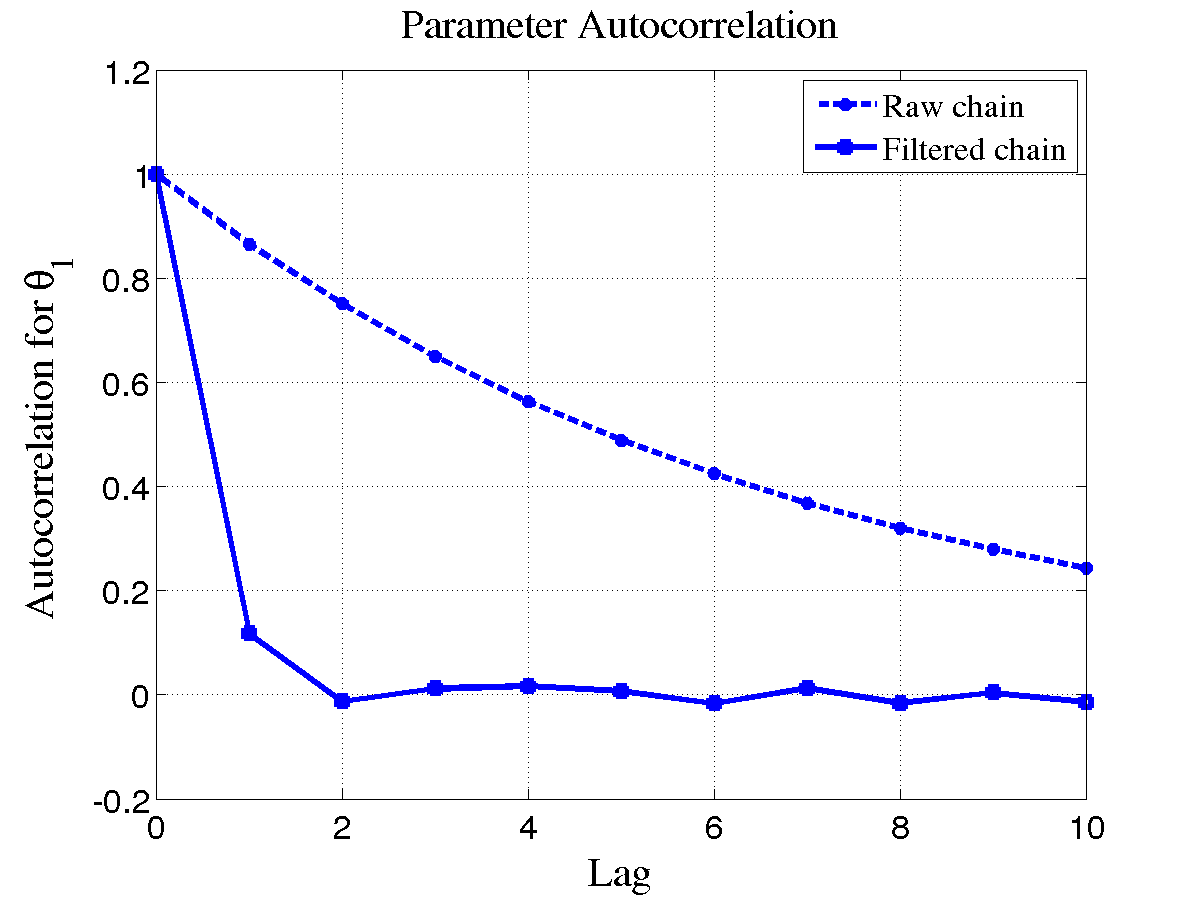
\includegraphics[scale=0.35]{figs/simple_ip_autocorrelation_raw_filt_theta1.png}}
%\subfloat[$\theta_2$]{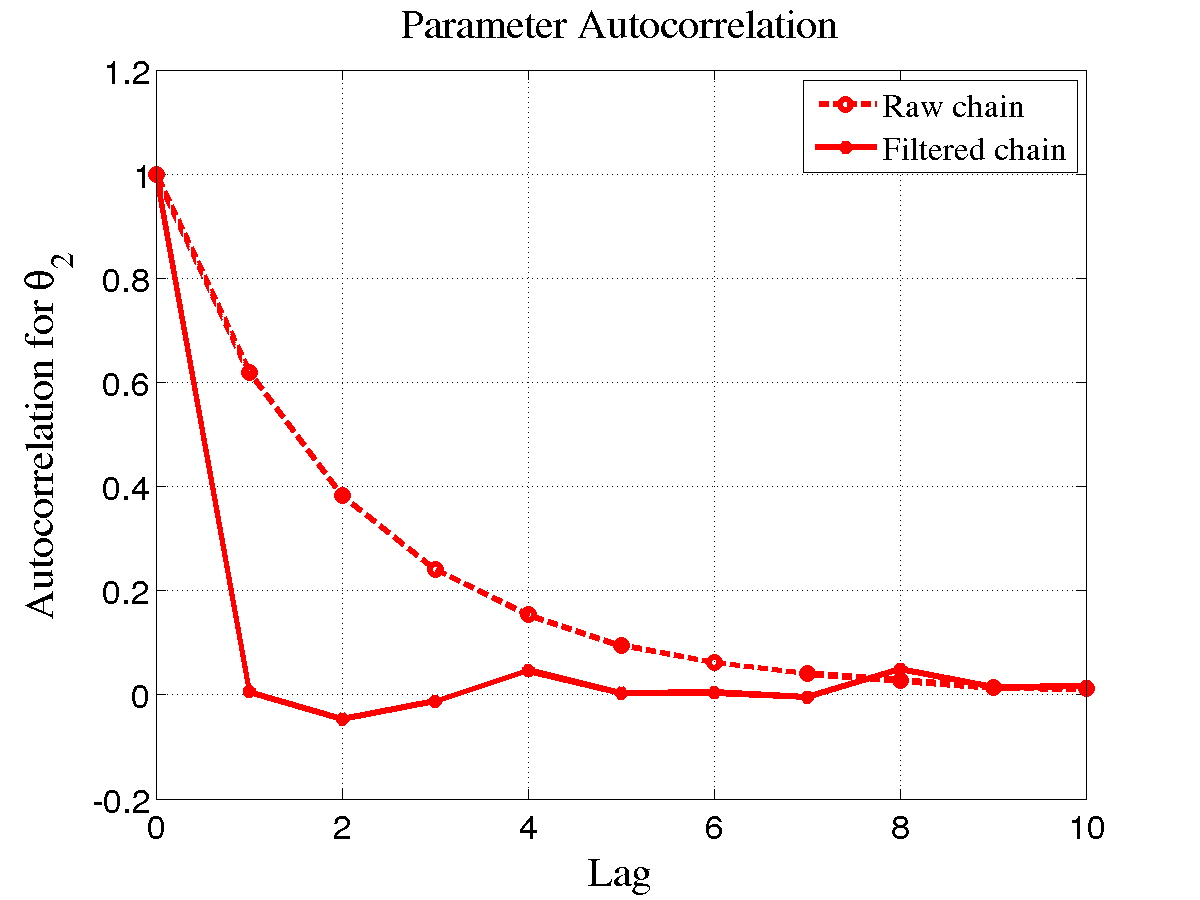
\includegraphics[scale=0.35]{figs/simple_ip_autocorrelation_raw_filt_theta2.png}}
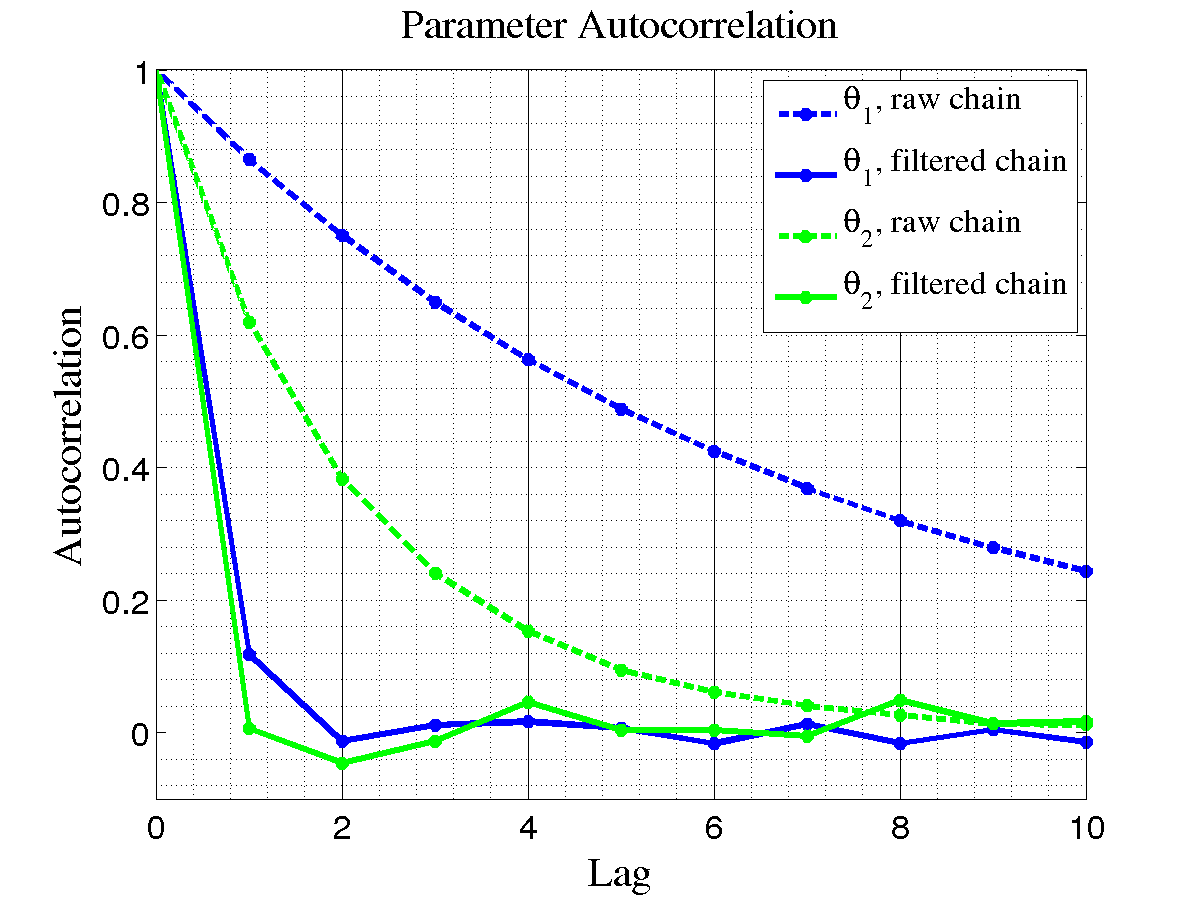
\includegraphics[scale=0.35]{figs/simple_ip_autocorrelation_raw_filt.png}
\vspace{-10pt}
\caption{
Autocorrelation plots obtained with QUESO for the SIP. }
\label{fig:simple_sip_autocorrelation_raw_filt}
\end{figure}


\subsubsection{KDE Plots}

Matlab function \verb+[f,xi] = ksdensity(x)+ (kernel smoothing density estimate) computes a probability density estimate of the sample in the vector \texttt{x}. \texttt{f} is the vector of density values evaluated at the points in \texttt{xi}. The estimate is based on a normal kernel function, using a window parameter (`width') that is a function of the number of points in \texttt{x}. The density is evaluated at 100 equally spaced points that cover the range of the data in x.  In order to estimate the KDE of the parameters, it is used together with the option `\verb+pdf+'. 

\begin{lstlisting}[label=matlab:ip_kde,caption={Matlab code for the KDE plots displayed in the left of Figure \ref{fig:simple_sip_kde}.}]
% Inside Matlab
% Raw chain
>> [f,x] = ksdensity(ip_mh_rawChain_unified(:,1),'function','pdf');
>> [f2,x2] = ksdensity(ip_mh_rawChain_unified(:,2),'function','pdf');
>> x_p1=sort(ip_mh_rawChain_unified(:,1)); %analytical
>> f_p1=(exp(-(x_p1+1).*(x_p1+1)/8))/2/sqrt(2*pi);
>> x_p2=sort(ip_mh_rawChain_unified(:,1));
>> f_p2=(exp(-(x_p2-2).*(x_p2-2)/2))/sqrt(2*pi);
>> plot(x,f,'b',x2,f2,'g','linewidth',4);
>> hold;
>> plot(x_p1,f_p1,'--k',x_p2,f_p2,'-k','linewidth',2);
>> h=legend('\theta_1', '\theta_2', 'analytical (\theta_1)', 'analytical (\theta_2)', 'location', 'northwest');
\end{lstlisting}

% \begin{lstlisting}[label=matlab:ip_kde,caption={Matlab code for the KDE plots displayed in Figure \ref{fig:simple_sip_kde}.}]
% % inside Matlab
% % theta_1
% >> [f,xi] = ksdensity(ip_mh_rawChain_unified(:,1),'function','pdf');
% >> x=ip_mh_rawChain_unified(:,1);
% >> x=sort(x);
% >> plot(x,(exp(-(x+1).*(x+1)/8))/2/sqrt(2*pi),'--k',xi,f,'-b','linewidth',3);
% >> title('Parameter Kernel Density Estimation (raw chain)','fontname', 'Times', 'fontsize',20);
% >> ylabel('Posterior marginal PDF','fontname', 'Times', 'fontsize',20);
% >> xlabel('\theta_1','fontname', 'Times', 'fontsize',20);
% >> h=legend('Analytical','QUESO','location','northeast');
% 
% % theta_2
% >> fprintf(1,' Plotting KDE - raw  <press any key>\n');
% >> [f,xi] = ksdensity(ip_mh_rawChain_unified(:,2),'function','pdf');
% >> x=ip_mh_rawChain_unified(:,2);
% >> x=sort(x);
% >> plot(x,(exp(-(x-2).*(x-2)/2))/sqrt(2*pi),'--k',xi,f,'-r','linewidth',3);
% >> title('Parameter Kernel Density Estimation (raw chain)','fontname', 'Times', 'fontsize',20);
% >> ylabel('Posterior marginal PDF','fontname', 'Times', 'fontsize',20);
% >> xlabel('\theta_2','fontname', 'Times', 'fontsize',20);
% >> h=legend('Analytical','QUESO','location','northeast');
% \end{lstlisting}

%Figure \ref{fig:sip_gravity_kde_raw} is created by using Matlab commands presented in Listing \ref{matlab:kde} above.
\begin{figure}[htpb]
\centering 
% \subfloat[]{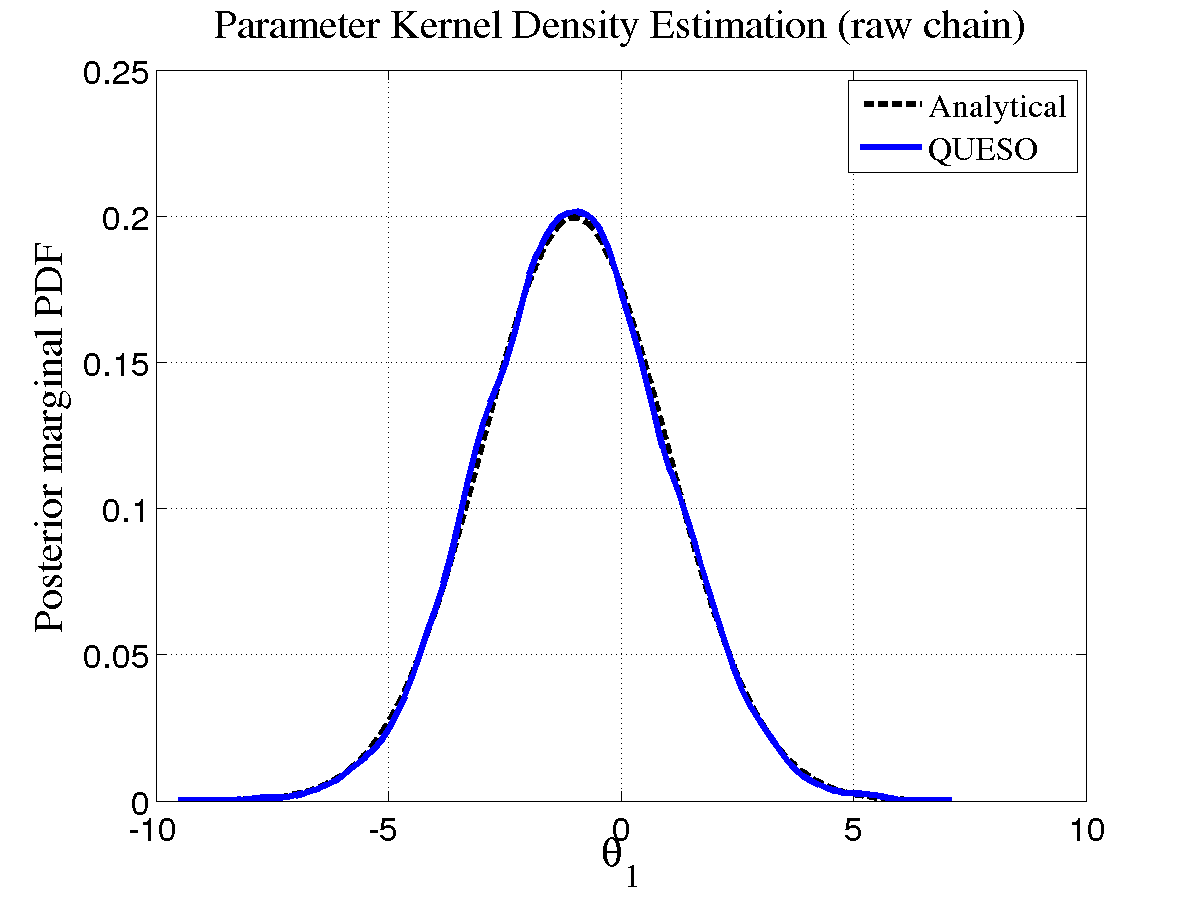
\includegraphics[scale=0.35]{figs/simple_ip_kde_theta1.png}}
% \subfloat[]{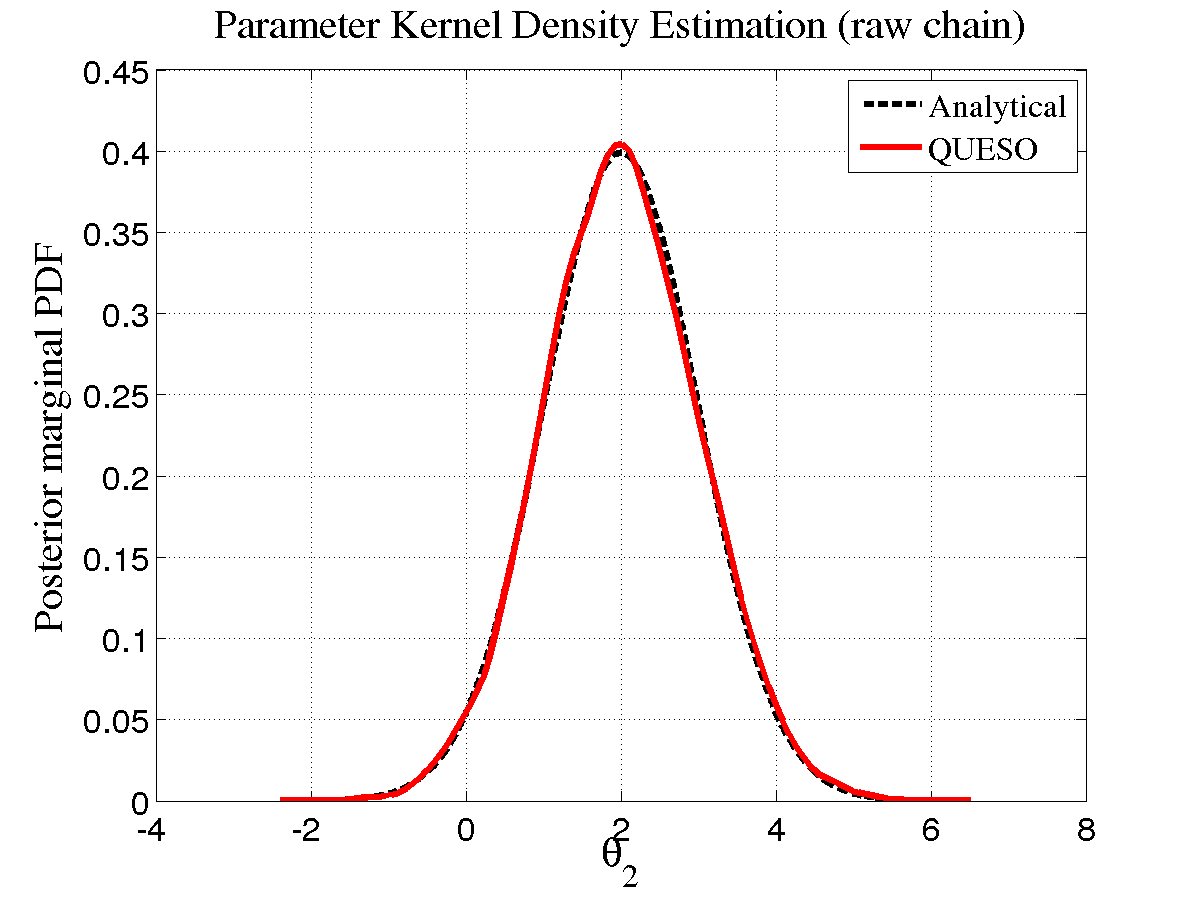
\includegraphics[scale=0.35]{figs/simple_ip_kde_theta2.png}}
\subfloat[Raw chain]{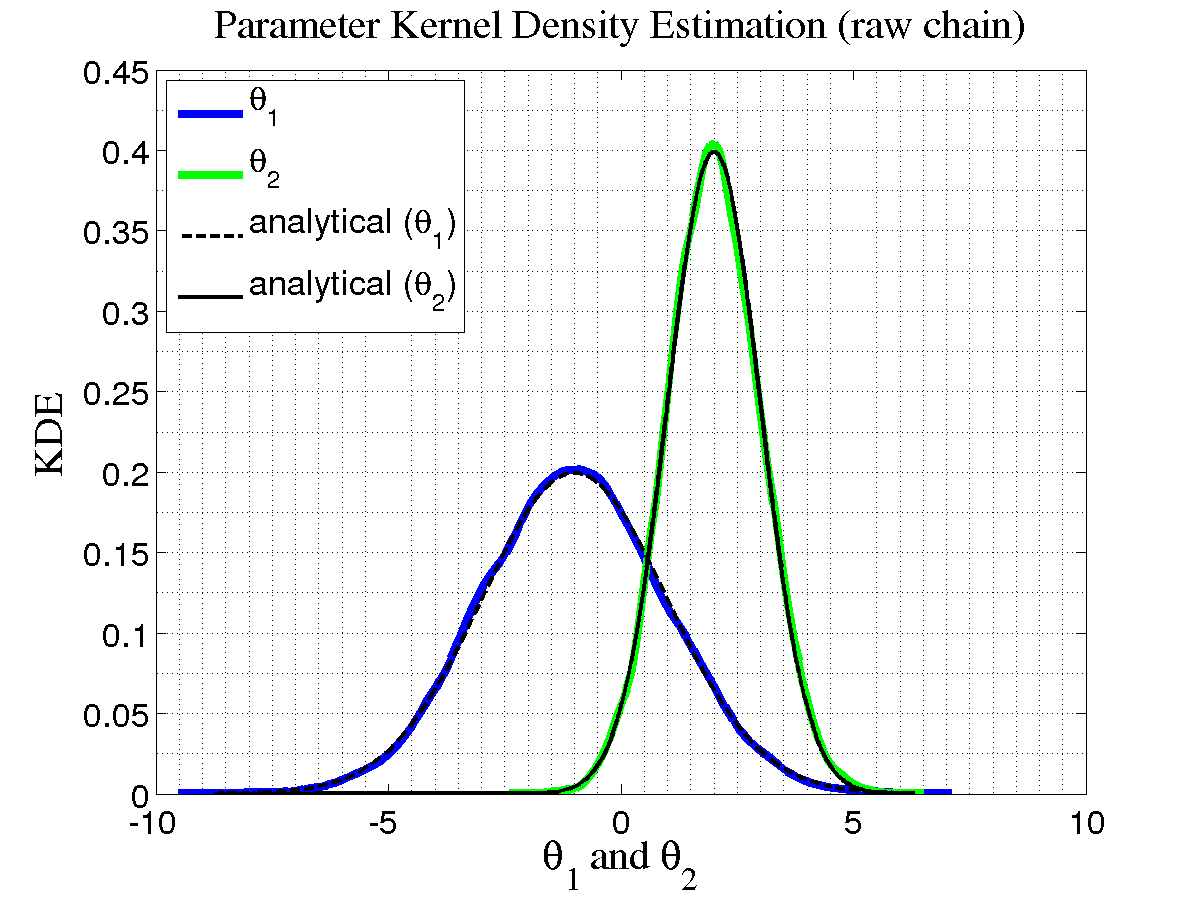
\includegraphics[scale=0.35]{figs/simple_ip_kde_raw.png}}
\subfloat[Filtered chain]{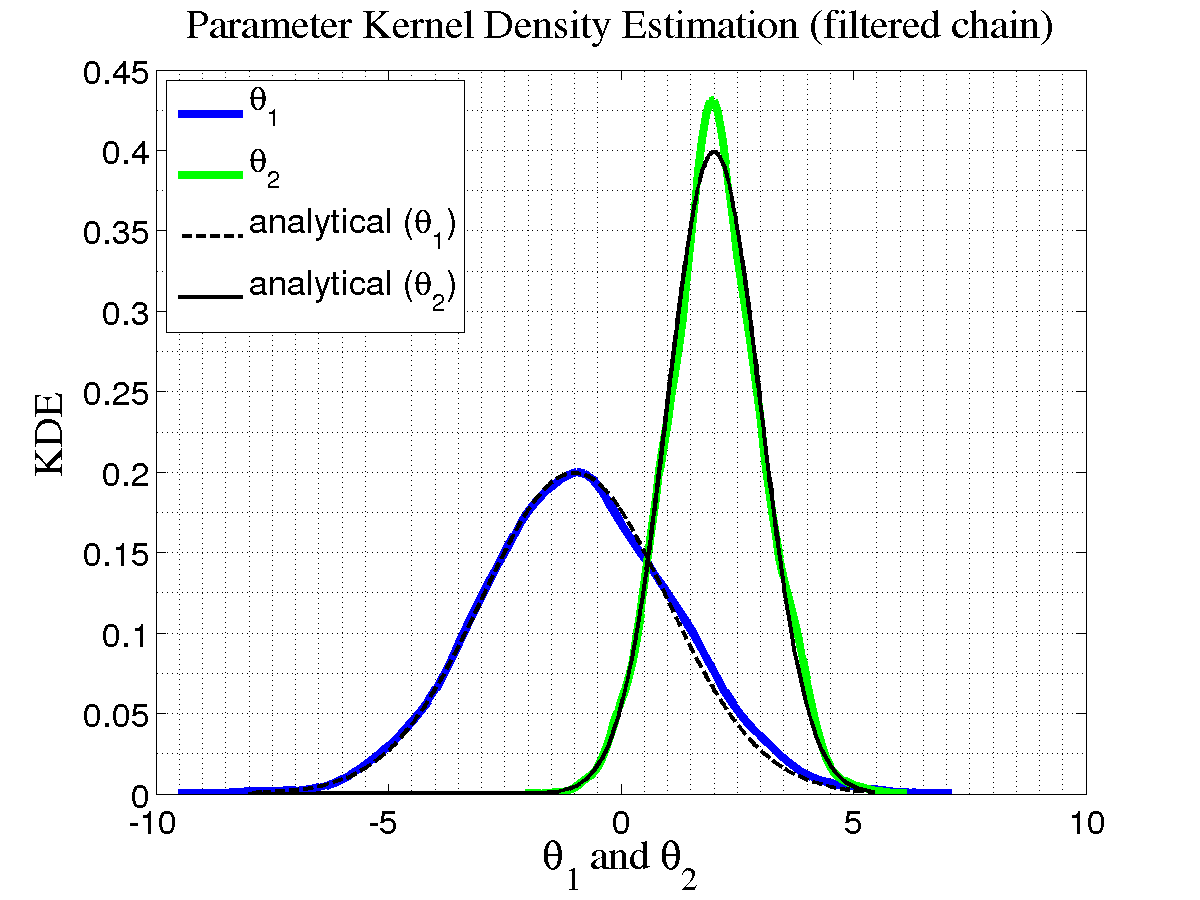
\includegraphics[scale=0.35]{figs/simple_ip_kde_filt.png}}
\vspace*{-10pt}
\caption{Kernel Density Estimation. QUESO results for estimation of the KDE of $\theta_1$ and $\theta_2$ are plotted against the analytical expressions $\pi_{\text{post}}(\theta_1)  =  \frac{1}{2\sqrt{2\pi}} \exp\left(-\frac{1}{8}(\theta_1+1)^2 \right)$  and $\pi_{\text{post}}(\theta_2)  =  \frac{1}{ \sqrt{2\pi}} \exp\left(-\frac{1}{2}(\theta_2-2)^2 \right)$, respectively.}
\label{fig:simple_sip_kde}
\end{figure}


\subsubsection{Covariance and Correlation Matrices}

Matlab function \verb+cov+ calculates the covariance matrix for a data matrix (where each column represents a separate quantity), 
and \verb+corr+ calculates the correlation matrix.

Listing \ref{matlab:cov_matrix} presents the Matlab steps for calculating the covariance and correlation matrices for the parameters $\theta_1$ and $\theta_2$.

\newpage

\begin{lstlisting}[label=matlab:ip_cov_matrix,caption={Matlab code for finding covariance and correlation matrices.}]
% inside Matlab
>> cov_matrix_theta1_theta2 = cov(ip_mh_rawChain_unified)

cov_matrix_theta1_theta2 =

    3.8729    0.0259
    0.0259    1.0050
    
>> corr_matrix_theta1_theta2 = corr(ip_mh_rawChain_unified)

corr_matrix_theta1_theta2 =

    1.0000    0.0132
    0.0132    1.0000    
\end{lstlisting}




\section{\texttt{simpleStatisticalForwardProblem}}\label{sec:example_sfp}

In this simple statistical forward problem (SFP), suppose that the quantity of interest $\mathbf{q}$ is a function of a random variable $\bv{\theta}$ of two parameters, namely $\bf{q}:\mathbb{R}^2\rightarrow\mathbb{R}$ such as:
\begin{equation}\label{eq-example-q}
\mathbf{q}(\boldsymbol{\theta}) = \theta_1+\theta_2,\quad\forall\boldsymbol{\theta}=(\theta_1,\theta_2)\in\mathbb{R}^2.
\end{equation}

Suppose also that the parameters in $\theta$ have Gaussian distribution with mean $\bv{\mu}$ and covariance matrix $\bf{C}$ given by:
\begin{equation}\label{eq-example-mu-sfp}
\boldsymbol{\mu} = 
\left(\begin{array}{c}
-1 \\
2
\end{array}\right)
\quad
\text{and}
\quad
\mathbf{C} = 
\left[\begin{array}{cc}
4 & 0 \\
0 & 1
\end{array}\right].
\end{equation}


Notice that since the solution $\mathbf{Q}$ of this SFP is the sum of two random variables $\boldsymbol{\Theta}_1$ and $\boldsymbol{\Theta}_2$, and since these two random variables independent Gaussian by assumption, should have:
\begin{equation}\label{eq-example-E}
E[\mathbf{Q}] = E[\boldsymbol{\Theta}_1] + E[\boldsymbol{\Theta}_2] = -1 + 2 = 1
\end{equation}
and
\begin{equation}\label{eq-example-V}
V[\mathbf{Q}] = V[\boldsymbol{\Theta}_1] + V[\boldsymbol{\Theta}_2] = 4 + 1 = 5
\end{equation}
where $E$ and $V$ indicate expectation and variance, respectively. Thus the analytical expression for the solution $\bf{Q}$ is this SFP is the one-dimensional Gaussian distribution of mean 1 and variance 5:
\begin{equation}\label{eq-example-sfp-analytical}
{\bf Q}(x)=   \frac{1}{ \sqrt{10\pi}} \exp\left(-\frac{1}{10}(x-1)^2 \right)
\end{equation}


In this example, we use QUESO Monte Carlo algorithm to sample from the QoI given in Equation (\ref{eq-example-q}) and analyze it. 
Since the parameters have known independent Gaussian distributions, the results obtained by QUESO via sampling the QoI, in Equation (\ref{eq-example-q}), should match the Gaussian distribution given in Equation (\ref{eq-example-sfp-analytical}).


\paragraph*{Note:} Due to the possibility to compare QUESO sampling algorithms to an analytical expression, this example is also used in the verification procedures and regression tests within QUESO. In fact it is the second part of the test \verb+tests/t02_sip_sfp+.


\subsection{Running the Example}\label{sec:sfp-run}
 
To run the executable provided (available after QUESO installation), enter the following commands:
\begin{lstlisting}[label={},caption={}]
$ cd $HOME/LIBRARIES/QUESO-0.47.1/
$ cd examples/simpleStatisticalForwardProblem
$ rm outputData/*
$ ./exSimpleStatisticalForwardProblem_gsl example.inp    
$ matlab
   $ simple_fp_plots      # inside matlab
   $ exit                 # inside matlab
$ ls -l outputData/*.png
 simple_fp_autocorrelation_qoi.png  simple_fp_chain_pos_param.png  
 simple_fp_hist_qoi.png             simple_fp_cdf_qoi.png
 simple_fp_chain_pos_qoi.png        simple_fp_kde_qoi.png
\end{lstlisting}

As a result, the user should have created several of PNG figures containing marginal posterior PDF, chain positions of the parameters and the QoI, histogram, cumulative density distribution and autocorrelation. The name of the figure files have been chosen to be informative, as shown in the Listing above.



\subsection{Example Code}\label{sec:code-sfp}

The source code for the SFP example is composed of 5 files:
\texttt{simple\_sfp\_example\_main.C} (Listing~\ref{code:sfp-main-c}),
\texttt{simple\_sfp\_example\_qoi.h} and \texttt{simple\_sfp\_example\_qoi.C} (Listings \ref{code:sfp-qoi-h} and~\ref{code:sfp-qoi-c}),
\texttt{simple\_sfp\_example\_compute.h}  and \texttt{simple\_sfp\_example\_compute.C} (Listings \ref{code:sfp-compute-h} and \ref{code:sfp-compute-c}).


\lstinputlisting[caption=File \texttt{simple\_sfp\_example\_main.C.}, label={code:sfp-main-c}, linerange={29-1000}]{../../examples/simpleStatisticalForwardProblem/src/simple_sfp_example_main.C}

\lstinputlisting[caption=File \texttt{simple\_sfp\_example\_qoi.h}., label={code:sfp-qoi-h}, linerange={28-1000}]{../../examples/simpleStatisticalForwardProblem/src/simple_sfp_example_qoi.h}

\lstinputlisting[caption=File \texttt{simple\_sfp\_example\_qoi.C}., label={code:sfp-qoi-c}, linerange={29-1000}]{../../examples/simpleStatisticalForwardProblem/src/simple_sfp_example_qoi.C}

\lstinputlisting[caption=File \texttt{simple\_sfp\_example\_compute.h.}, label={code:sfp-compute-h}, linerange={28-1000}]{../../examples/simpleStatisticalForwardProblem/src/simple_sfp_example_compute.h}

\lstinputlisting[caption={File \texttt{simple\_sfp\_example\_compute.C}.}, label={code:sfp-compute-c}, linerange={29-1000},numbers=left]{../../examples/simpleStatisticalForwardProblem/src/simple_sfp_example_compute.C}
 


\subsection{Input File}\label{sec:sfp-input-file}

In the case of a SFP, QUESO expects a list of options for Monte Carlo algorithm,
together with options for QUESO environment; such as the name of the output files and which sub-environments will write to to them. 
Note that the names of the variables have been designed to be informative:
\begin{description}\vspace{-8pt}
\item[ \texttt{env}:] refers to QUESO environment; \vspace{-8pt}
\item[ \texttt{fp}:] refers to forward problem;\vspace{-8pt}
\item[ \texttt{mc}:] refers to Monte Carlo;\vspace{-8pt}
\item[ \texttt{pseq}:] refers to the parameter sequence; and\vspace{-8pt}
\item[ \texttt{qseq}:] refers to the quantity of interest sequence.
\end{description}

The options used for solving this simple SFP are displayed in Listing \ref{code:sfp-input-file}.


\lstinputlisting[caption={File name \texttt{simple\_sfp\_example.inp} with options for QUESO library used in application code (Listings \ref{code:sfp-main-c}--\ref{code:sfp-compute-c}})., 
label={code:sfp-input-file},]{../../examples/simpleStatisticalForwardProblem/tests/test_2013_08_27/simple_sfp_example.inp}



\subsection{Create your own Makefile}\label{sec:sfp-makefile}

 
Listing \ref{code:makefile} presents a Makefile, named `\texttt{Makefile\_sfp\_example\_margarida}', that may be used to compile the code and create the executable \verb+simple_sfp_example+. Naturally, it must be adapted to the user's settings, i.e., it has to have the correct paths for the user's libraries that have actually been used to compile and install QUESO.

\lstinputlisting[caption={Makefile for the application code in Listings \ref{code:sfp-main-c}--\ref{code:sfp-compute-c}},  label={code:sfp-makefile},language={bash}]{../../examples/simpleStatisticalForwardProblem/src/Makefile_sfp_example_margarida}

Thus, to compile, build and execute the code, the user just needs to run the following commands in the same directory where the files are:
\begin{lstlisting}
$ cd HOME/LIBRARIES/QUESO-0.47.1/examples/simpleStatisticalForwardProblem 
$ export LD_LIBRARY_PATH=$LD_LIBRARY_PATH:\
  $HOME/LIBRARIES/gsl-1.15/lib/:\
  $HOME/LIBRARIES/boost-1.53.0/lib/:\
  $HOME/LIBRARIES/hdf5-1.8.10/lib:\
  $HOME/LIBRARIES/QUESO-0.47.1/lib 
$ make -f Makefile_sfp_example_margarida 
$ ./simple_sfp_example simple_sfp_example.inp
\end{lstlisting}

The `\verb+export+' instruction above is only necessary if the user has not saved it in his/her \verb+.bashrc+ file. 


\subsection{Data Post-Processing and Visualization}\label{sec:sfp-results}

This section discusses the results computed by QUESO with the code of Section \ref{sec:code-sfp}, and shows how to use Matlab for the post-processing of the data generated by QUESO when solving SFPs. Only the essential Matlab commands are presented; for the complete/detailed codes, please refer to file '\verb+simple_fp_plots.m+'.

According to the specifications of the input file in Listing~\ref{code:sfp-input-file}, a folder named `\verb+outputData+' containing the following files should be created: \verb+display_sub0.txt, fp_p_seq.m,+ \linebreak \verb+fp_p_seq_sub0.m, fp_q_seq.m, fp_q_seq_sub0.m,+ and \verb+sfpOutput_sub0.m+.

The code bellow shows how to load the data provided by QUESO during the solution process of the SFP described, in the form of chains of positions.
\begin{lstlisting}[caption={Matlab code for loading the data in both parameter and QoI chains of the SFP.}]
% inside Matlab
>> clear all
>> fp_p_seq.m
>> fp_q_seq.m
\end{lstlisting}


Alternatively, the user may call the file \texttt{simple\_fp\_plots.m}, which contains the above commands, together with a variety of others, for data visualization:
\begin{lstlisting}[caption={Matlab code for loading the data in both parameter and QoI chains of the SFP, by calling the file \texttt{simple\_fp\_plots.m}.}]
% inside Matlab
>> clear all
>> simple_fp_plots
\end{lstlisting}




\subsubsection{Histogram Plots}

In order to plot a histogram of the QoI, you may use the pre-defined Matlab function \verb+hist+.
The Matlab code presented in Listing \ref{matlab:fp_hist_qoi} below shows how to create the Figure~\ref{fig:fp_qoi_hist}.

\begin{lstlisting}[label=matlab:fp_hist_qoi,caption={Matlab code for the QoI histogram plot.}]
% inside Matlab
>> fp_q_seq  %if commands of Listings 3.19/3.20 have not been called
>> nbins=20;
>> hist(fp_mc_QoiSeq_unified,nbins);
>> title('QoI Histogram','fontsize',20);
>> xlabel('QoI=\theta_1+\theta_2','fontname', 'Times', 'fontsize',20)
>> ylabel('Frequency','fontsize',20);
\end{lstlisting}

\begin{figure}[htb]
\centering 
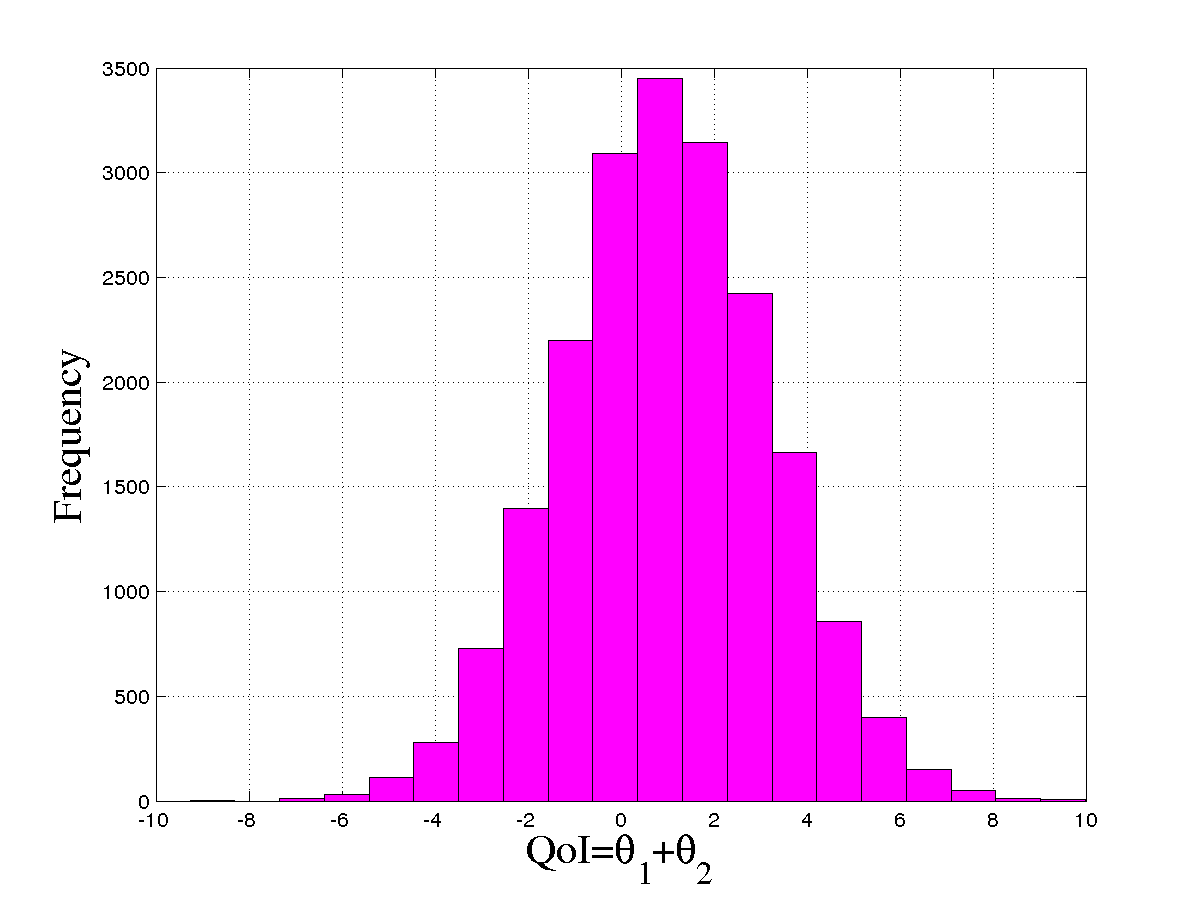
\includegraphics[scale=0.35]{figs/simple_fp_hist_qoi.png}
\vspace{-10pt}
\caption{QoI histogram.}
\label{fig:fp_qoi_hist}
\end{figure}

\subsubsection{KDE Plot}

Matlab function \verb+ksdensity+ (Kernel smoothing density estimate) together with the option `\verb+pdf+' may be used to estimate the KDE of the QoI. 

\begin{lstlisting}[label=matlab:fp_kde_qoi,caption={Matlab code for the KDE displayed in Figure \ref{fig:simple_sfp_kde}}]
% inside Matlab
>> fp_q_seq  %if commands of Listing 5.19 have not been called
>> [fi,xi] = ksdensity(fp_mc_QoiSeq_unified,'function','pdf');
>> x=sort(fp_mc_QoiSeq_unified);
>> mu=1;
>> sigma2=5;
>> f=(exp(-(x-mu).*(x-mu)/sigma2/2))/sqrt(2*pi*sigma2);
>> plot(xi,fi,'-m','linewidth',4);
>> hold;
>> plot(x,f,'--k','linewidth',2);
>> h=legend('QoI = \theta_1+\theta_2','analytical','location','northwest');
\end{lstlisting}


%Figure \ref{fig:sip_gravity_kde_raw} is created by using Matlab commands presented in Listing \ref{matlab:kde} above.
\begin{figure}[htpb]
\centering 
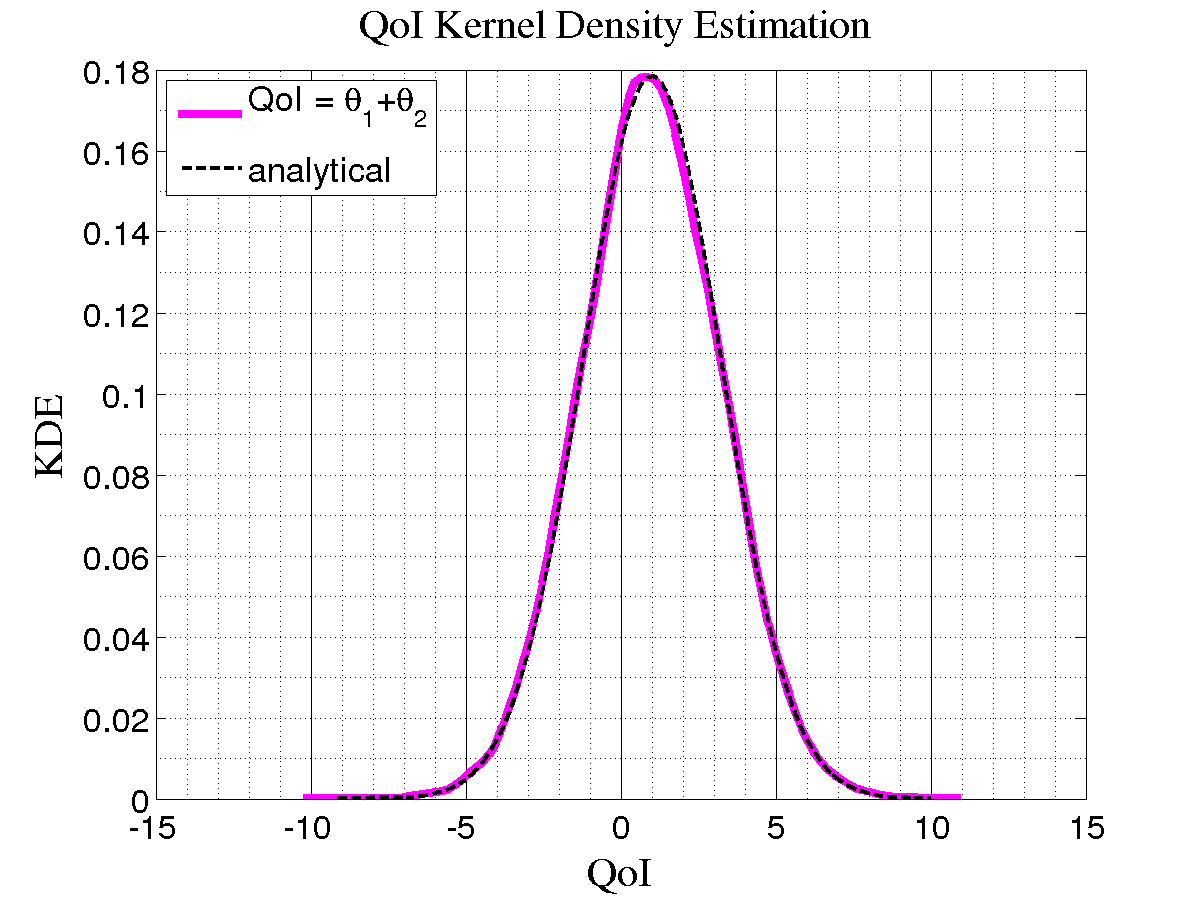
\includegraphics[scale=0.35]{figs/simple_fp_kde_qoi.png}
\vspace{-10pt}
\caption{Kernel Density Estimation. QUESO results are plotted against the PDF of a Gaussian distribution $Q(x)=   \frac{1}{ \sqrt{10\pi}} \exp\left(-\frac{1}{10}(x-1)^2 \right)$, where $\mu=1$ and $\sigma^2=5$.}
\label{fig:simple_sfp_kde}
\end{figure}


\subsubsection{CDF Plot}

Matlab function \verb+ksdensity+ with \verb+'cdf'+ option may also be used for plotting the Cumulative Distribution Function of the QoI.

\begin{lstlisting}[label=matlab:fp_cdf_qoi,caption={Matlab code for the QoI CDF plot displayed in Figure \ref{fig:simple_sfp_cdf}.}]
% inside Matlab
>> fp_q_seq  %if commands of Listing 5.19 have not been called
>> [f,xi] = ksdensity(fp_mc_QoiSeq_unified,'function','cdf');
>> plot(xi,f,'-m','linewidth',3)
\end{lstlisting}

\begin{figure}[htpb]
\centering 
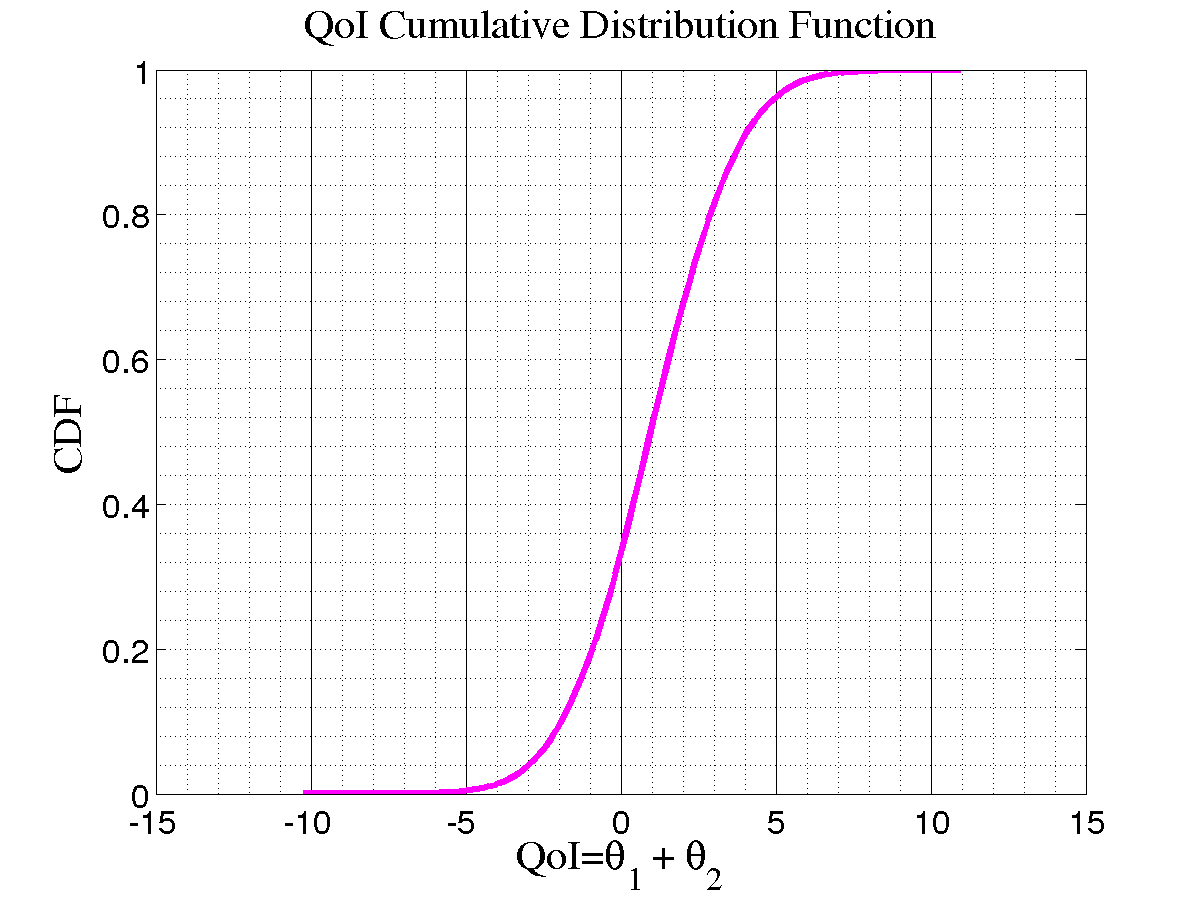
\includegraphics[scale=0.35]{figs/simple_fp_cdf_qoi.png}
\vspace*{-10pt}
\caption{Cumulative Distribution Function.}
\label{fig:simple_sfp_cdf}
\end{figure}



\section{\texttt{gravity}}\label{sec:example_gravity}

This section presents an example of how to use QUESO in order to develop an application that solves a statistical inverse problem and
a statistical forward problem, where the solution of the former serves as input to the later. During the SIP, the acceleration due to gravity for an object in free fall near the surface of the Earth is inferred. During the SFP, the distance traveled by a projectile launched at a given angle and altitude is calculated using the calibrated magnitude of the acceleration of gravity.


In this section we describe a statistical forward problem  of predicting the  described in Section \ref{sec:gravity-ip}.

\subsection{Statistical Inverse Problem}\label{sec:gravity-ip}

% Near the surface of the Earth, an object in free fall in a vacuum will accelerate at approximately $9.8 m/s^2$, independent of its mass.
% With air resistance acting upon an object that has been dropped, mass, drag coefficient and even relative surface may become important
% (if the fall is from sufficient altitude) in the calculation of gravity.

%The vertical motion of an object falling a small distance close to the surface of the planet can be approximated to have
%uniform gravitational field without air resistance, as long as the force of gravity on the object is much greater than the force of air resistance.

%Therefore a convenient, simplified 
A possible deterministic mathematical model for the vertical motion of an object in free fall near the surface of the Earth is given by
\begin{equation}\label{eq:gravity01}
h(t)=-\frac{1}{2} g t^2 + v_0 t + h_0.
\end{equation}
where
$v_0$ [$m/s$] is the initial velocity,
$h_0$ [$m$] is the initial altitude,
$h(t)$ [$m$] is the altitude with respect to time,
$t$ [$s$] is the elapsed time, and
$g$ [$m/s^2$] is the magnitude of the acceleration due to gravity (the parameter which cannot be directly measured and will be statistically inferred).



\subsubsection{Experimental Data}
We assume that the experiment of allowing an object to fall from different altitudes with zero initial velocity has been repeatedly conducted (See Figure \ref{fig:free_fall}). The data collected, e.g.  $\mathbf{d}$, is displayed in Table \ref{table:data}; the standard deviations, $\sigma$'s, refer to the uncertainties in the measured times during the experiment execution~\cite{interactagram}. 



\begin{figure}[!h]
\centering
\input{rawfigs/free_fall.latex}
\vspace*{-8pt}
\caption{An object falls from altitude $h_0$ with zero initial velocity ($v_0=0$).}
\label{fig:free_fall}
\end{figure}

\begin{table}[htp]%% Data from data02.dat 
\caption{Measurement data $\mathbf{d}$ of size $n_d=14$.
The object falls from altitude $h_0$ in $t$ seconds, with standard deviation of $\sigma$ seconds in the time measurement~\cite{interactagram}.
}
% \specialrule{.4pt}{10pt}{4pt}
\vspace{-8pt}
\begin{center}
\begin{tabular}{ccc}
\toprule
% $(h_0-h)$ [$m$] & $t$ [$s$]  & $\sigma$ [$s$]\\
altitude [$m$] & time [$s$]  & Std. Dev. $\sigma$ [$s$]\\
\midrule
\midrule
$~$10	&	1.41	&	0.02	\\
$~$20	&	2.14	&	0.12	\\
$~$30	&	2.49	&	0.02	\\
$~$40	&	2.87	&	0.01	\\
$~$50	&	3.22	&	0.03	\\
$~$60	&	3.49	&	0.01	\\
$~$70	&	3.81	&	0.03	\\
$~$80	&	4.07	&	0.03	\\
$~$90	&	4.32	&	0.03	\\
100	&	4.47	&	0.05	\\
110	&	4.75	&	0.01	\\
120	&	4.99	&	0.04	\\
130	&	5.16	&	0.01	\\
140	&	5.26	&	0.09	\\
\bottomrule
\end{tabular}
\end{center}
\label{table:data}
\end{table}



\subsubsection{The Prior RV, Likelihood and Posterior RV}

In a straightforward classical interpretation of Bayesian inference, the prior signifies the modeler's honest opinion about the unknown.
For the gravity inference problem, let's assume that gravity varies uniformly in the interval [8,11], or, in other words, we chose uniform prior distribution in that interval:

\begin{equation}\label{eq-g-prior}
\pi_{\text{prior}}=\mathcal{U}(8,11).
\end{equation}


We choose the usual likelihood function:
\begin{equation}\label{eq:like02}
\pi_{\text{like}}(\mathbf{d} | \boldsymbol{\theta})
\varpropto
\exp
\left\{
-\frac{1}{2}
[\mathbf{y}(\boldsymbol{\theta})-\mathbf{d}]^T
\left[\mathbf{C}(\boldsymbol{\theta})\right]^{-1}
[\mathbf{y}(\boldsymbol{\theta})-\mathbf{d}]
\right\},
\end{equation}
where $\mathbf{C}(\boldsymbol{\theta})$ is a given covariance matrix, $\mathbf{d}$ denotes experimental data, $\mathbf{y}(\boldsymbol{\theta})$ is the model output data.

Recalling the deterministic model for the acceleration of gravity (\ref{eq:gravity01}) with zero initial velocity,  the information provided in Table \ref{table:data}, and Equation (\ref{eq:like02}); and, additionally, invoking the nomenclature used in Section \ref{sec:statistical_concepts}, we have:
\begin{equation}\label{eq:like03}
\boldsymbol{\theta} \stackrel{\text{\small{def.}}}{=} g,
%------------ 
\quad
\mathbf{y}(\boldsymbol{\theta})= 
\left[
\begin{array}{c}
\sqrt{\dfrac{2 h_1}{g}}\\	
\sqrt{\dfrac{2 h_2}{g}}\\	
\vdots\\	
\sqrt{\dfrac{2 h_{n_d}}{g}}
\end{array}
\right],
%------------ 
\quad 
\mathbf{d} = 
\left[
\begin{array}{c}
t_1    \\
t_2    \\ 
\vdots \\	
t_{n_d}
\end{array}
\right],
%------------ 
\quad
\mathbf{C}(\boldsymbol{\theta})=
\left[
\begin{array}{cccc}
\sigma^2_1 & 0	        & \cdots & 0 \\
0          & \sigma^2_2 & \cdots & 0 \\
\vdots     & \vdots     & \ddots & 0 \\
0          & 0          & \cdots & \sigma^2_{n_d}
\end{array}
\right],
\end{equation}
where $n_d=14$ is the number of data points in Table \ref{table:data}.

Now we are ready to evoke Bayes' formula in order to obtain the posterior PDF $\pi_{\text{post}}(\boldsymbol{\theta})$:
\begin{equation}\label{eq-Bayes-g}
\pi_{\text{post}}(\boldsymbol{\theta}|\mathbf{d})\varpropto  \pi_{\text{like}}(\mathbf{d}|\boldsymbol{\theta}) \, \pi_{\text{prior}}(\boldsymbol{\theta}).
\end{equation}


\subsection{Statistical Forward Problem}


Projectile motion refers to the motion of an object projected into the air at an angle, e.g. a soccer ball being kicked, a baseball being thrown, or an athlete long jumping. Supposing the object does not have a propulsion system and neglecting air resistance, then the only force acting on the object is a constant gravitational acceleration $g$.


A possible deterministic two-dimensional mathematical model for the vertical motion of an object projected from near the surface of the Earth is given by
\begin{align}\label{eq:fwd01}
v_x &= v_{0x} \\ %&= v_{0} \cos(\alpha), \\
v_y &= v_{0y} - gt \\ %&= v_{0} \sin(\alpha) - gt,\\
  x &= v_{0x}t \\ %&= v_{0} \cos(\alpha) t, \\
  h &= h_0 + v_{0y}t - \frac{1}{2} g t^2  %&= v_{0} \sin(\alpha) t - \frac{1}{2} g t^2.
\end{align}
where
$h_0$ is the initial height, $x=x(t)$ is the distance traveled by the object, $\bv{v_0}=(v_{0x},v_{0y})$ is the initial velocity,
$v_{0x} = v_{0} \cos(\alpha)$, $v_{0y} = v_{0} \sin(\alpha)$, and $v_0=\|\bv{v_0}\|^2$.
%
Figure \ref{fig:projectile} displays the projectile motion of an object in these conditions.
\begin{figure}[!h]
\centering
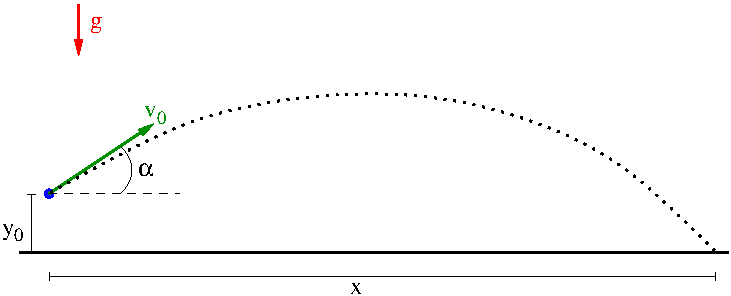
\includegraphics[scale=1]{figs/projectile}
\vspace*{-8pt}
\caption{Object traveling with projectile motion. }
\label{fig:projectile}
\end{figure}


%Assume that we want to describe the motion of such an object, starting at time $t = 0$, ... and velocity that makes an angle $\alpha$ with the $x$-axis.


For this example, we assume that $h_0 =0$ m, $\alpha = \pi/4$ radians, $v_0 = 5$ m/s, all deterministic variables; and $g$ is the solution of the SIP described in Section \ref{sec:gravity-ip}.

Since a PDF is assigned to parameter $g$; thus, the output of the mathematical model (\ref{eq:fwd01}) becomes a random variable, thus we have a statistical forward problem. 

\subsubsection{The Input RV, QoI Function and Output RV}
 
The input random variable for the statistical forward problem is the acceleration of gravity $g$, which is also the solution (posterior PDF) of the inverse problem described in Section \ref{sec:gravity-ip}. The output random variable for this example is the distance $x$ traveled by an object in projectile motion. Note that, since there is uncertainty in the parameter $g$ ($g$ is given as a PDF), one can expect that this uncertainty will be propagated to $x$, which will also be given as a PDF.

Combining the expressions in Equation \ref{eq:fwd01} and rearranging them, we have that QoI function for $x$ %(i.e. the final model for the distance traveled by an object in projectile motion) 
is: 
\begin{equation}\label{eq:fp_deterministic}
x=\dfrac{ v_0 \cos \alpha }{g} \left( v_0  \sin \alpha  + \sqrt{ ( v_0  \sin \alpha)^2 + 2g\, y_0 }\right).                                                                                        
\end{equation}
where $y$ is the distance traveled and our quantity of interest (QoI). 



\subsection{Running the Example}\label{sec:gravity-run}
 
To run the executable provided (available after QUESO installation), enter the following commands:
\begin{lstlisting}[label={},caption={}]
$ cd $HOME/LIBRARIES/QUESO-0.47.1/examples/gravity
$ rm outputData/*
$ ./gravity_gsl gravity_inv_fwd.inp
\end{lstlisting}

The console output of the program is:
\begin{lstlisting}[caption={Console output of program \texttt{gravity\_gsl}}, label={code:console_output},language={bash}]
kemelli@violeta:~/LIBRARIES/QUESO-0.47.1/examples/gravity$ ./gravity_gsl gravity_inv_fwd.inp 
---------------------------------------------------------------------
QUESO Library: Version = 0.47.1 (47.1)

Development Build

Build Date   = 2013-04-29 17:05
Build Host   = violeta
Build User   = kemelli
Build Arch   = x86_64-unknown-linux-gnu
Build Rev    = 38998M

C++ Config   = mpic++ -g -O2 -Wall

Trilinos DIR = 
GSL Libs     = -L/home/kemelli/LIBRARIES/gsl-1.15/lib -lgsl -lgslcblas -lm
GRVY DIR     = 
GLPK DIR     = 
HDF5 DIR     = /home/kemelli/LIBRARIES/hdf5-1.8.10
--------------------------------------------------------------------------------------------------------------
Beginning run at Mon Apr 29 17:27:32 2013

MPI node of worldRank 0 has fullRank 0, belongs to subEnvironment of id 0, and has subRank 0
MPI node of worldRank 0 belongs to sub communicator with full ranks 0
MPI node of worldRank 0 also belongs to inter0 communicator with full ranks 0, and has inter0Rank 0


Beginning run of 'Gravity + Projectile motion' example at Mon Apr 29 17:27:32 2013

 my fullRank = 0
 my subEnvironmentId = 0
 my subRank = 0
 my interRank = 0

Beginning 'SIP -> Gravity estimation' at Mon Apr 29 17:27:32 2013

Solving the SIP with Metropolis Hastings

Beginning 'SFP -> Projectile motion' at Mon Apr 29 17:27:33 2013

Solving the SFP with Monte Carlo

Ending run of 'Gravity + Projectile motion' example at Mon Apr 29 17:27:33 2013

Ending run at Mon Apr 29 17:27:33 2013
Total run time = 1 seconds
kemelli@violeta:~/LIBRARIES/QUESO-0.47.1/examples/gravity$ 
\end{lstlisting}


In order to generate chain plots, histograms, KDEs, etc., the user may use Matlab/GNU Octave and call the following command lines:
\begin{lstlisting}
$ matlab
   $ gravity_plots_ip      # inside matlab
   $ gravity_plots_fp      # inside matlab
   $ exit                  # inside matlab
$ ls -l outputData/*.png
  sfp_gravity_autocorrelation.png  sfp_gravity_cdf.png
  sfp_gravity_chain_pos.png        sfp_gravity_hist.png
  sfp_gravity_kde.png              sip_gravity_autocorrelation_raw_filt.png
  sip_gravity_cdf_filt.png         sip_gravity_cdf_raw.png
  sip_gravity_chain_pos_filt.png   sip_gravity_chain_pos_raw.png
  sip_gravity_hist_filt.png        sip_gravity_hist_raw.png
  sip_gravity_kde_filt.png         sip_gravity_kde_raw.png
\end{lstlisting}

As a result, the user should have created several of PNG figures containing marginal posterior PDF, chain positions of the parameters and the QoI, histogram, cumulative density distribution and autocorrelation. The name of the figure files have been chosen to be informative, as shown in the Listing above.



\subsection{Gravity Example Code}\label{sec:gravity_code}

The source code for the SIP and the SFP is composed of 7 files.
Three of them are common for both problems: \texttt{gravity\_main.C, gravity\_compute.h} and \texttt{gravity\_compute.C}; they combine both problems and use the solution of the SIP (the posterior PDF for the gravity) as an input for the SFP and are presented, respectively, in Listings \ref{code:gravity_main}, \ref{code:gravity_compute_h} and \ref{code:gravity_compute_C}.
Two of files specifically  handle the SIP: \texttt{gravity\_likelihood.h}, and \texttt{gravity\_likelihood.C}, and are displayed in Listings \ref{code:gravity_like_h} and \ref{code:gravity_like_C}. Finally, the files specific for the SFP are \texttt{gravity\_qoi.h} and \texttt{gravity\_qoi.C}, and they are presented in Listings \ref{code:gravity_qoi_h} and \ref{code:gravity_qoi_C}.

\lstinputlisting[caption=File \texttt{gravity\_main.C.}, label=code:gravity_main, linerange={27-1000}]{../../examples/gravity/src/gravity_main.C}
 
\lstinputlisting[caption=File \texttt{gravity\_compute.h.}, label=code:gravity_compute_h, linerange={33-1000}]{../../examples/gravity/src/gravity_compute.h}

\lstinputlisting[caption={File \texttt{gravity\_compute.C}. The first part of the code (lines 37--113) handles the statistical forward problem, whereas the second part of the code (lines 115--163) handles the statistical forward problem.\\}, label=code:gravity_compute_C, linerange={27-1000},numbers=left]{../../examples/gravity/src/gravity_compute.C}

\lstinputlisting[caption=File \texttt{gravity\_likelihood.h}., label=code:gravity_like_h, linerange={33-1000}]{../../examples/gravity/src/gravity_likelihood.h}

\lstinputlisting[caption=File \texttt{gravity\_likelihood.C}., label=code:gravity_like_C, linerange={27-1000}]{../../examples/gravity/src/gravity_likelihood.C}

\lstinputlisting[caption=File \texttt{gravity\_qoi.h}., label=code:gravity_qoi_h, linerange={33-1000}]{../../examples/gravity/src/gravity_qoi.h}

\lstinputlisting[caption=File \texttt{gravity\_qoi.C}., label=code:gravity_qoi_C, linerange={33-96}]{../../examples/gravity/src/gravity_qoi.C}

\subsection{Input File}\label{sec:gravity-input-file}

QUESO reads an input file for solving statistical problems.
In the case of a SIP, it expects a list of options for MCMC, while in case of SFP it expects a list of options for Monte Carlo. The  input file `\texttt{gravity\_inv\_fwd.inp} used in this example is presented in Listing \ref{code:gravity_inv_fwd}.

\lstinputlisting[caption=Some options for QUESO library used in application code (Listings \ref{code:gravity_main}-\ref{code:gravity_like_C})., label={code:gravity_inv_fwd},]{../../examples/gravity/tests/test_2013_01_22/gravity_inv_fwd.inp}


 

Moreover, for the gravity inverse problem, one may notice that QUESO will use the Metropolis-Hastings algorithm to sample the posterior PDF
(indicated by the prefix \texttt{mh\_}in the variable names) without adaptive steps
(indicated by the zero value assigned to the variable \linebreak \texttt{ip\_mh\_am\_initialNonAdaptInterval}, which can also be achieved by setting zero to \linebreak
\verb+ip_mh_am_adaptInterval+) and with delayed rejection (indicated by the one-value assigned to the variable \texttt{ip\_mh\_dr\_maxNumExtraStages}).



 
\subsection{Create your own Makefile}\label{sec:gravity-makefile}



Listing \ref{code:makefile} presents a Makefile, named \texttt{Makefile\_example\_violeta}, that may be used to compile the code and create the executable \verb+gravity_gsl+. Naturally, it must be adapted to the user's settings, i.e., it has to have the correct paths for the user's libraries that were actually used to compile and install QUESO (see Sections \ref{sec:Pre_Queso}--\ref{sec:install_Queso_make}).

\lstinputlisting[caption={Makefile for the application code in Listings \ref{code:gravity_main}-\ref{code:gravity_like_C}},  label={code:makefile},language={bash}]{../../examples/gravity/src/Makefile_example_violeta}




\subsection{Running the Gravity Example with Several Processors}

Even though the application described in Section \ref{sec:gravity_code} is a serial code, it is possible to run it using more than one processor, i.e., in parallel mode. 
Supposing the user's workstation has $N_p=8$ processors, then, the user my choose to have $N_s =$ 8, 4 or 2 subenvironments. This complies with the requirement that the total number of processors in the environment must be a multiple of the specified number of subenvironments.

Thus, to build and run the application code with $N_p = 8$, and $N_s=8$ subenvironments, the must set the variable \texttt{env\_numSubEnvironments = 8} in the input file (Listing~\ref{code:gravity_inv_fwd}) and enter the following command lines: 



\begin{lstlisting}[caption={}, label={},language={bash}]
cd $HOME/LIBRARIES/QUESO-0.47.1/examples/gravity/
mpirun -np 8 ./gravity_gsl gravity_inv_fwd.inp
\end{lstlisting}


The steps above will create a total number of 8 raw chains, of size defined by the variable \texttt{ip\_mh\_rawChain\_size}. QUESO internally combines these 8 chains into a single chain of size $8\; \times\,$\texttt{ip\_mh\_rawChain\_size} and saves it in a file named according to the variable \texttt{ip\_mh\_rawChain\_dataOutputFileName}. 
QUESO also provides the user with the option of writing each chain -- handled by its corresponding processor -- in a separate file, which is accomplished by setting the variable \texttt{ip\_mh\_rawChain\_dataOutputAllowedSet = 0 1 ... Ns-1}.\\

\noindent
{\bf Note:} Although the discussion in the previous paragraph refers to the raw chain of a SIP, the analogous is true for the filtered chains (SIP), and for the samples employed in the SFP (\texttt{ip\_mh\_filteredChain\_size},    \texttt{fp\_mc\_qseq\_size} and \texttt{fp\_mc\_qseq\_size}, respectively). 




\subsection{Data Post-Processing and Visualization}\label{sec:gravity-results}

 

According to the specifications of the input file in Listing~\ref{code:gravity_inv_fwd}, both a folder named \verb+outputData+ and a the following files should be generated:
\begin{verbatim}
sfp_gravity_sub0.m,         sip_gravity_sub0.m, 
sfp_gravity_p_seq.m,        sip_gravity_filtered_chain.m,,
sfp_gravity_p_seq_sub0.m    sip_gravity_filtered_chain_sub0.m,
sfp_gravity_qoi_seq.m,      sip_gravity_raw_chain.m,       
sfp_gravity_qoi_seq_sub0.m  sip_gravity_raw_chain_sub0.m,
display_env_sub0.txt 
\end{verbatim}

%The names of the files have been chosen to be informative.


%In this case, only one sub-environment (processor) has been used, thus, only one file of the type \verb+display_env_sub*+ is generated.
%

In this section, a convenient capability of QUESO of internally handling possible conflicts in chain size is presented. Recalling the input file \verb+gravity_inv_fwd.inp+ presented in Listing~\ref{code:gravity_inv_fwd}, one may notice that  the raw chain size for the SIP is chosen to have 20000 positions (\verb+ip_mh_rawChain_size = 20000+); the lag of the filtered chain is chosen to be 20 (\verb+ip_mh_filteredChain_lag = 20+) and the chain size for the SFP has 16384 positions (\verb+fp_mc_qseq_size = 16384+). Because the solution of the SIP, ie, the posterior PDF, is used as input PDF for the SFP, QUESO internally sets \verb+fp_mc_qseq_size = 20000+, as can be seen in the file \verb+display_env_sub0.txt+.  The file \verb+display_env_sub0.txt+ contains information from the subenvironment `0' that was generated during the run of the application code.

\subsubsection{Statistical Inverse Problem}

There are a few Matlab-ready commands that are very helpful tools for post-processing the data generated by QUESO when solving statistical inverse problems.
This section discusses the results computed by QUESO with the code of Section \ref{sec:gravity_code}, and shows how to use Matlab for the post-processing of such results.

\paragraph{Chain Plots}\

It is quite simple to plot, using Matlab, the chain of positions used in the DRAM algorithm implemented within QUESO. 
The sequence of Matlab commands presented in Listing \ref{matlab:chain} generates the graphic depicted in Figure \ref{fig:sip_gravity_chain_pos_raw}.
Figure~\ref{fig:sip_gravity_chain_pos_filtered} is obtained analogously. % by loading \verb+sip_gravity_filtered_chain+ and using  \verb+ip_mh_filtChain_unified+ inside \verb+plot+.

\begin{lstlisting}[label=matlab:chain,caption={Matlab code for the chain plot.}]
% inside Matlab
>> sip_gravity_raw_chain
>> plot(ip_mh_rawChain_unified)
>> ylabel('\theta=g','fontsize',20);
>> xlabel('Number of positions','fontsize',20);
>> title('DRAM Chain Positions (raw)','fontsize',20);
\end{lstlisting}

\begin{figure}[htb]
\centering 
\subfigure[Raw chain]{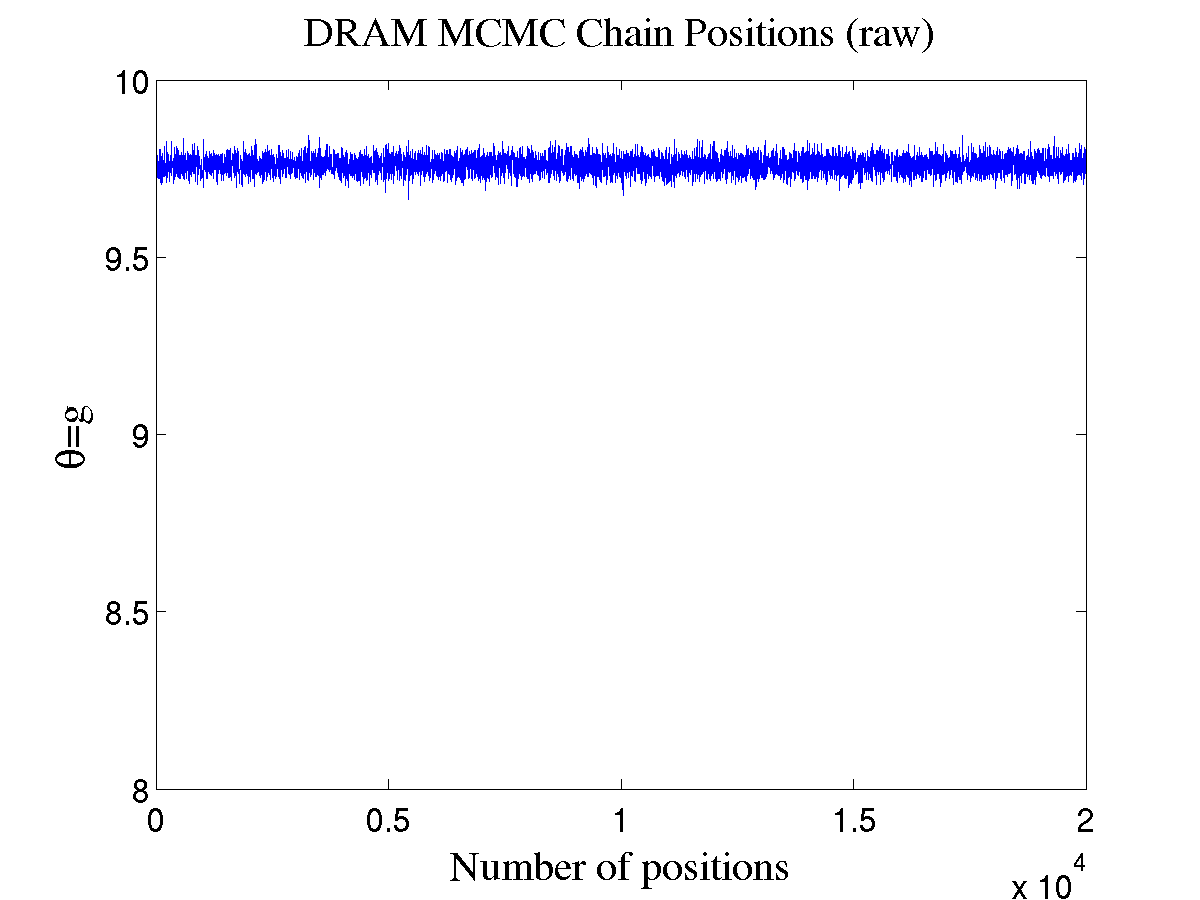
\includegraphics[scale=0.35]{figs/sip_gravity_chain_pos_raw.png}\label{fig:sip_gravity_chain_pos_raw}}
\subfigure[Filtered chain]{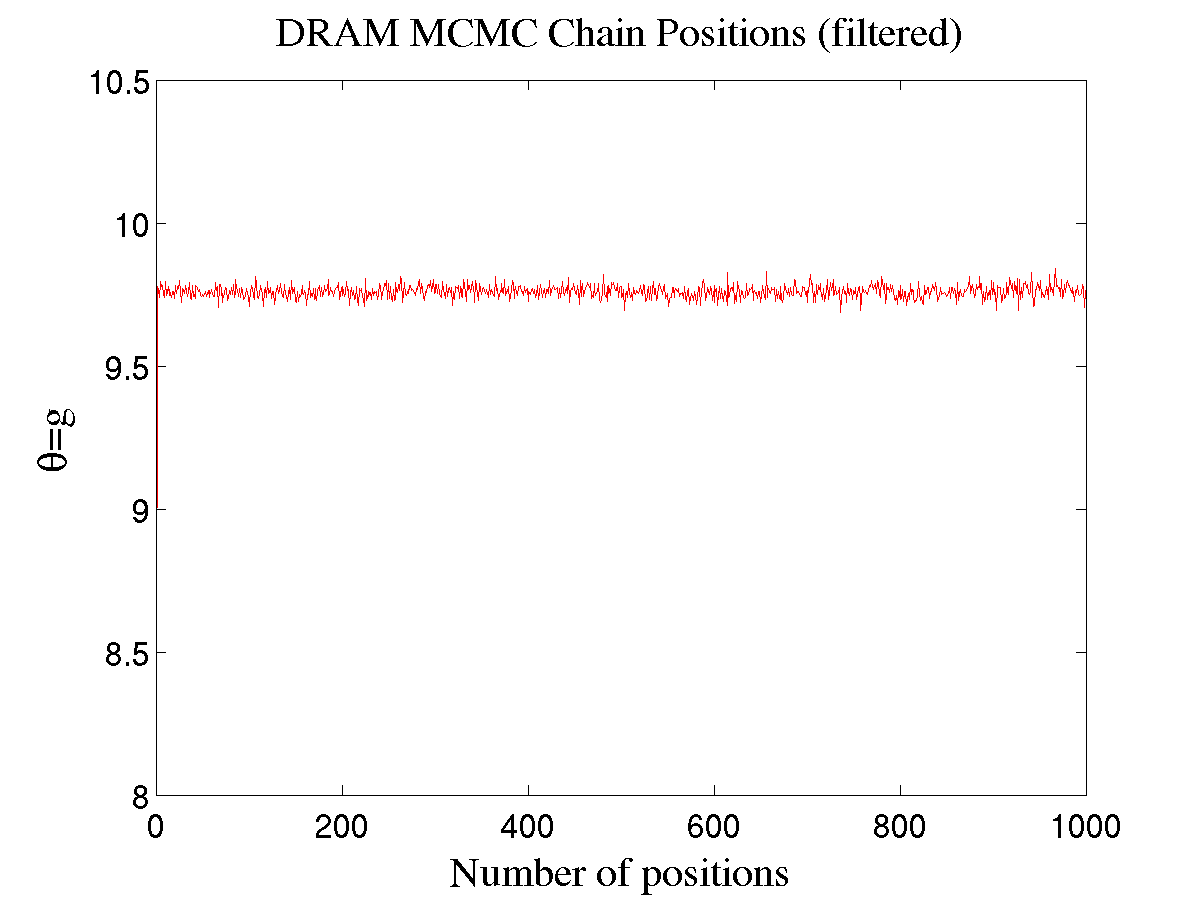
\includegraphics[scale=0.35]{figs/sip_gravity_chain_pos_filt.png}\label{fig:sip_gravity_chain_pos_filtered}}
\vspace*{-10pt}
\caption{MCMC raw chain with \chainsizeresults{} positions and a filtered chain with lag of 20 positions.}
\end{figure}

\paragraph{Histogram Plots}\

In order to plot histograms of the parameter using either the raw chain or the filtered chain, you simply have to use the pre-defined Matlab function \verb+hist+.
%The Matlab code presented in Listing \ref{matlab:hist} below shows how to create the Figure \ref{fig:sip_gravity_hist_raw};
%once more, Figure \ref{fig:sip_gravity_hist_filtered} is obtained by making suitable adjustments on that code.
%
\begin{lstlisting}[label=matlab:hist,caption={Matlab code for the histogram plot.}]
% inside Matlab
>> sip_gravity_raw_chain
>> nbins=100;
>> hist(ip_mh_rawChain_unified,nbins)
>> title('Parameter Histogram (raw chain)','fontsize',20);
>> xlabel('Gravity (m/s^2)','fontsize',20);
>> ylabel('Frequency','fontsize',20);
>> grid on;
\end{lstlisting}

\begin{figure}[htb]
\centering 
\subfigure[Raw chain]{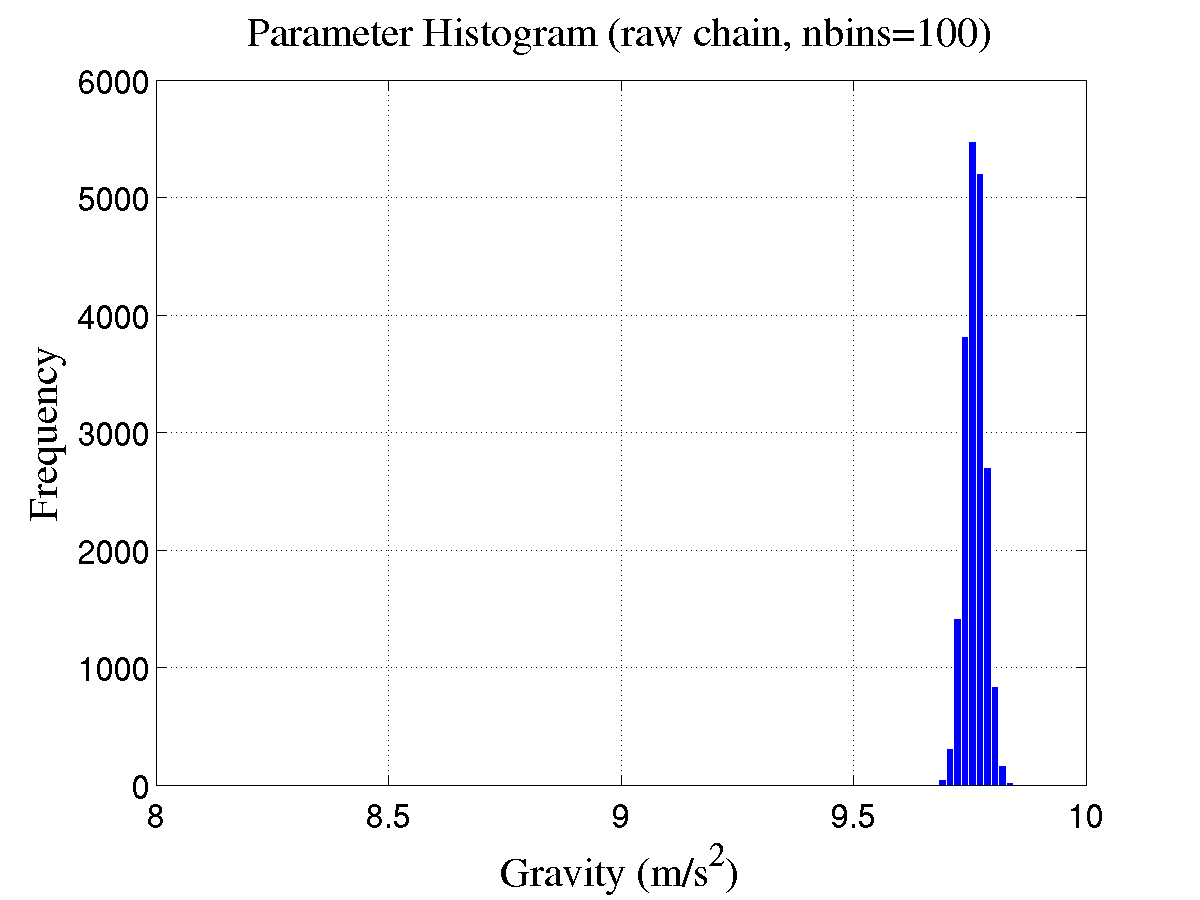
\includegraphics[scale=0.35]{figs/sip_gravity_hist_raw.png}\label{fig:sip_gravity_hist_raw}}
\subfigure[Filtered chain]{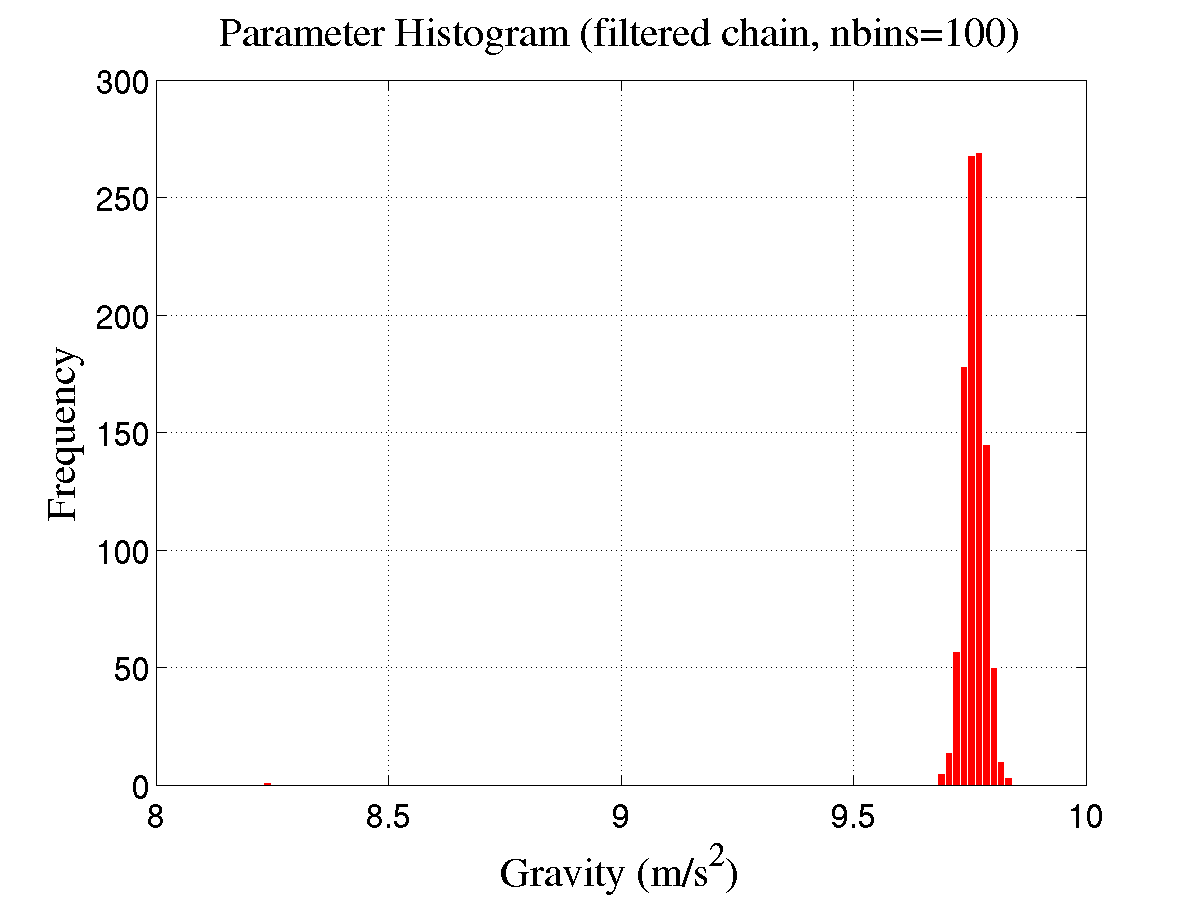
\includegraphics[scale=0.35]{figs/sip_gravity_hist_filt.png}\label{fig:sip_gravity_hist_filtered}}
\vspace*{-10pt}
\caption{Histograms of parameter $\theta=g$. }
\end{figure}

\paragraph{KDE Plots} \

Matlab function \verb+ksdensity+ (Kernel smoothing density estimate) together with the option \verb+'pdf'+ may be used for plotting the KDE of the parameter.
\begin{lstlisting}[label=matlab:kde,caption={Matlab code for the KDE plot.}]
% inside Matlab
>> sip_gravity_raw_chain
>> [f,xi] = ksdensity(ip_mh_rawChain_unified,'function','pdf');
>> plot(xi,f,'-b','linewidth',3)
>> title('Parameter Kernel Density Estimation','fontsize',20);
>> xlabel('Gravity (m/s^2)','fontsize',20);
>> ylabel('KDE','fontsize',20);
>> grid on;
\end{lstlisting}

%Figure \ref{fig:sip_gravity_kde_raw} is created by using Matlab commands presented in Listing \ref{matlab:kde} above.
\begin{figure}[htpb]
\centering 
\subfigure[Raw chain]{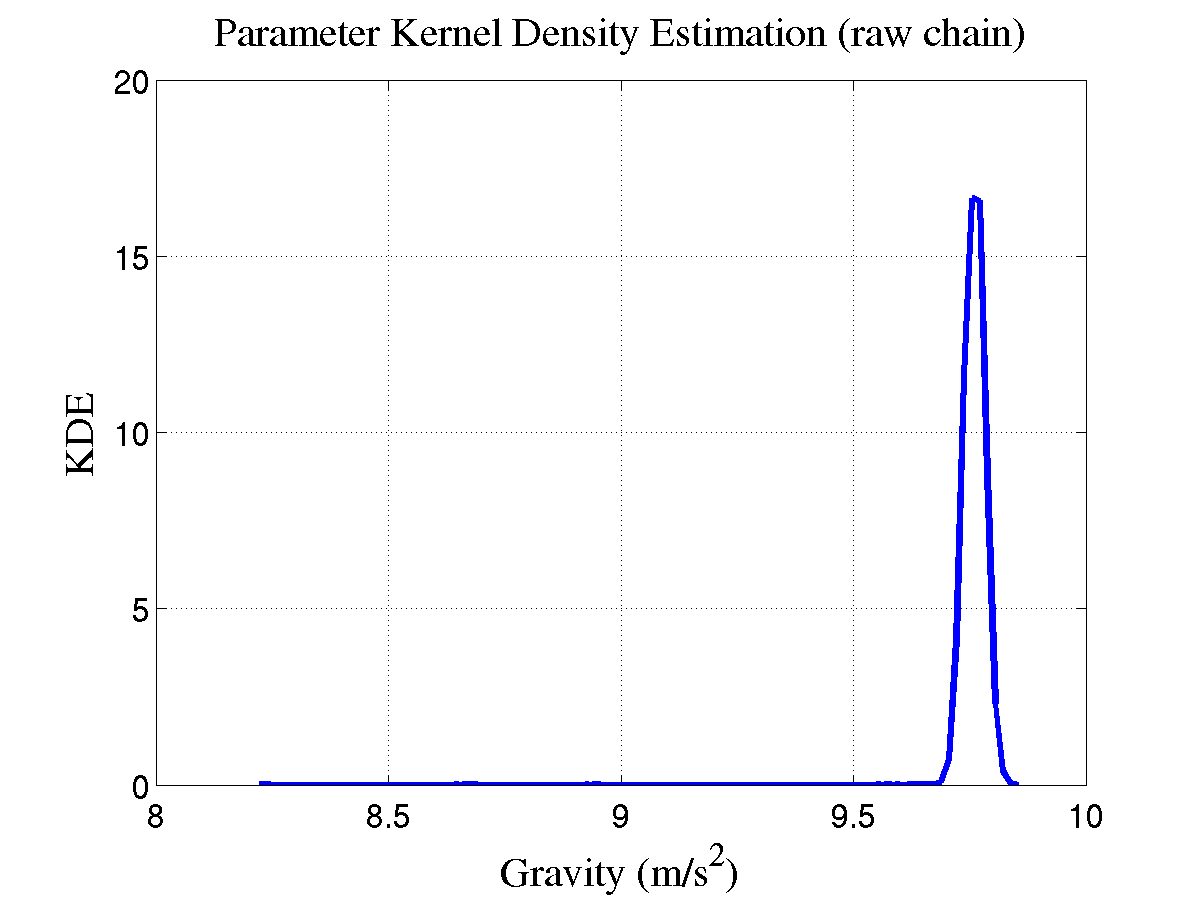
\includegraphics[scale=0.35]{figs/sip_gravity_kde_raw.png}\label{fig:sip_gravity_kde_raw}}
\subfigure[Filtered chain]{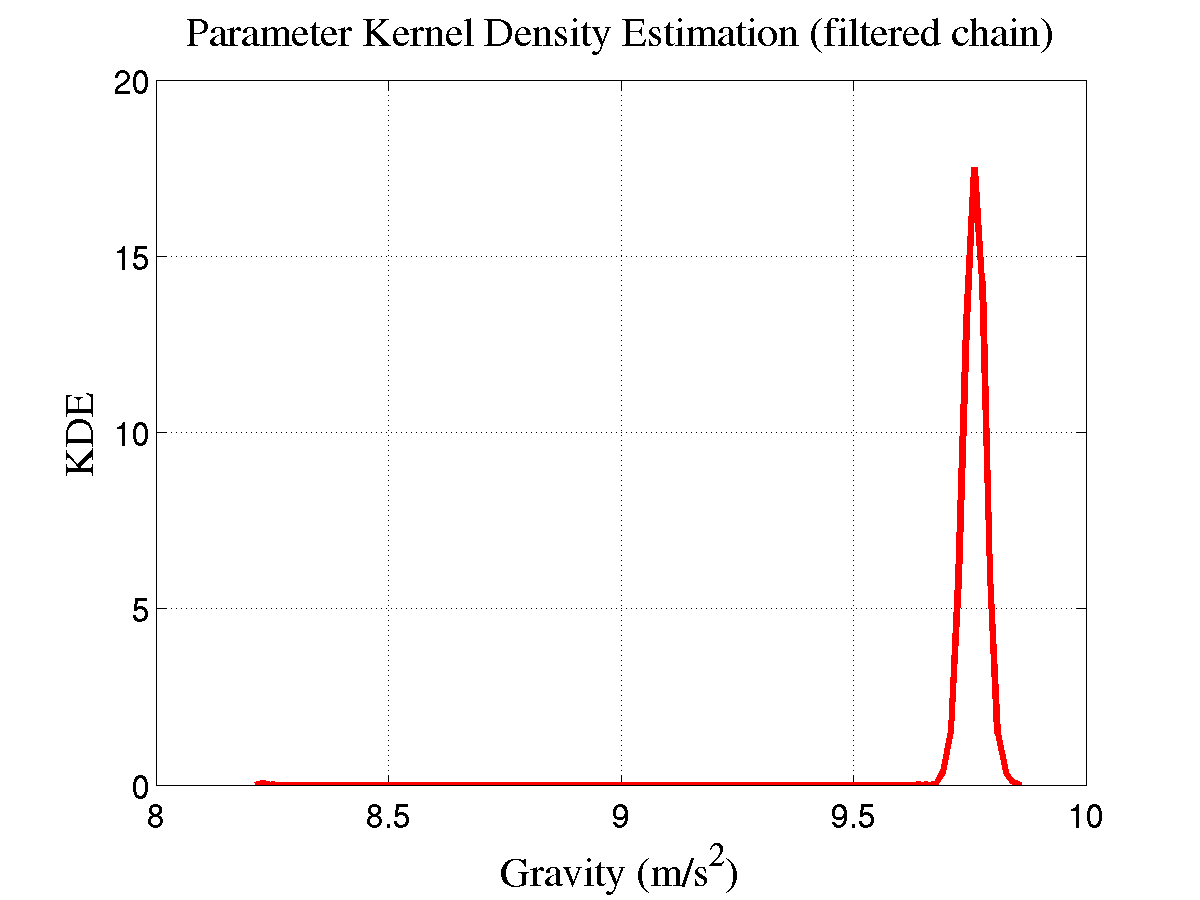
\includegraphics[scale=0.35]{figs/sip_gravity_kde_filt.png}\label{fig:sip_gravity_kde_filtered}}
\vspace*{-10pt}
\caption{Kernel Density Estimation. }
\end{figure}


% \subsubsection{Checking a KDE Plot Against Brute-Force Plot of the Likelihood Function}
% 
% See Figure \ref{fig:sip_gravity_compare_brute_force_unnormal}.
% %Figures \ref{fig:sip_gravity_compare_brute_force_unnormal} and \ref{fig:sip_gravity_compare_brute_force_normal} depict unnormalized and normalized KDE distributions
% %comparing the solution of the SIP provided by QUESO ($\pi_{\text{post}} (g)$) and the analytical (brute force) distribution.
% 
% \begin{figure}[htpb]
% \centering 
% %\subfigure[Unnormalized]{\includegraphics[scale=0.35]{figs/gravity_likelihood_brute_force_compare_post_pdf_0.png}\label{fig:sip_gravity_compare_brute_force_unnormal}}
% %\subfigure[Normalized]{\includegraphics[scale=0.35]{figs/gravity_likelihood_brute_force_compare_post_pdf_normalized0.png}\label{fig:sip_gravity_compare_brute_force_normal}}
% \subfigure{\includegraphics[scale=0.35]{figs/gravity_likelihood_brute_force_compare_post_pdf_0.png}\label{fig:sip_gravity_compare_brute_force_unnormal}}
% \vspace*{-10pt}
% \caption{Comparison of the posterior KDE for $g$ against the brute force calculation of the likelihood on a regular grid on $g$.
% }
% \end{figure}
% 
% %The code had to be slightly modified in order to replace QUESO sampling from the uniform distribution for the gravity with what we call a `brute force sampling'.
% %This brute force `sampling'  consists of recovering a pre-defined amount of values for $g$ from an equally spaced interval.
% %This is accomplished in lines 75 -- 100 of code \ref{code:gravity_compute_bruteforce_C}: it replaces Steps 4-6 (lines 100-150)
% %of the original application code provided in Algorithm \ref{code:gravity_compute_C}.
% 
% %\lstinputlisting[caption={Application code modified to `brute force' sampling from pre-defined interval.}, label={code:gravity_compute_bruteforce_C},  linerange={28-1000}]{../../brute_force/gravity_compute.C}
%  
% %Once more, Matlab function \verb+ksdensity+ (Kernel smoothing density estimate) may be used for plotting the KDE of the parameter.
% %The Matlab code below is responsible for the generation of Figure \ref{fig:sip_gravity_compare_brute_force_unnormal}.
% %Note that it reads the file \verb+gravity_likeli_brute_force.dat+, which is an output of the brute force code depicted in Listing \ref{code:gravity_compute_bruteforce_C}.
% %%
% %\begin{lstlisting}[label=matlab:kde_bruteforce,caption={Matlab code for the comparison of KDE plot from QUESO and `brute force'.}]
% %% inside Matlab
% %>> [g,like]=textread('gravity_likeli_brute_force.dat', '%f %f' );
% %>> [f,xi] = ksdensity(ip_mh_rawChain_unified,'function','pdf');
% %>> [haxes,hline1,hline2] = plotyy(xi,f,g,exp(like),'plot', 'plot');
% %>> axes(haxes(1));
% %>> ylabel('\pi_{post}(g) - QUESO/raw chain','fontname', 'Times', 'fontsize',20);
% %>> axes(haxes(2));
% %>> ylabel('\pi_{like}(g) -  brute force','fontname', 'Times', 'fontsize',20);
% %>> grid on;
% %>> title('Unnormalized distributions','fontname', 'Times', 'fontsize',20);
% %>> set(hline1,'linewidth',3);
% %>> set(hline2,'linewidth',3);
% %\end{lstlisting}


\paragraph{CDF Plots} \

Matlab function \verb+ksdensity+ (Kernel smoothing density estimate) with \verb+'cdf'+ option may also be used for plotting the Cumulative Distribution Function of the parameter.


\begin{lstlisting}[label=matlab:cdf,caption={Matlab code for the CDF plot.}]
% inside Matlab
>> sip_gravity_raw_chain
>> [f,xi] = ksdensity(ip_mh_rawChain_unified,'function','cdf');
>> plot(xi,f,'-b','linewidth',3)
>> title('Parameter Cumulative Distribution Function','fontsize',20);
>> xlabel('Gravity (m/s^2)','fontsize',20);
>> ylabel('CDF','fontsize',20);
>> grid on;
\end{lstlisting}

%Similarly, Figure \ref{fig:sip_gravity_cdf_raw} is created by using above Matlab commands.
\begin{figure}[ht]
\centering 
\subfigure[Raw chain]{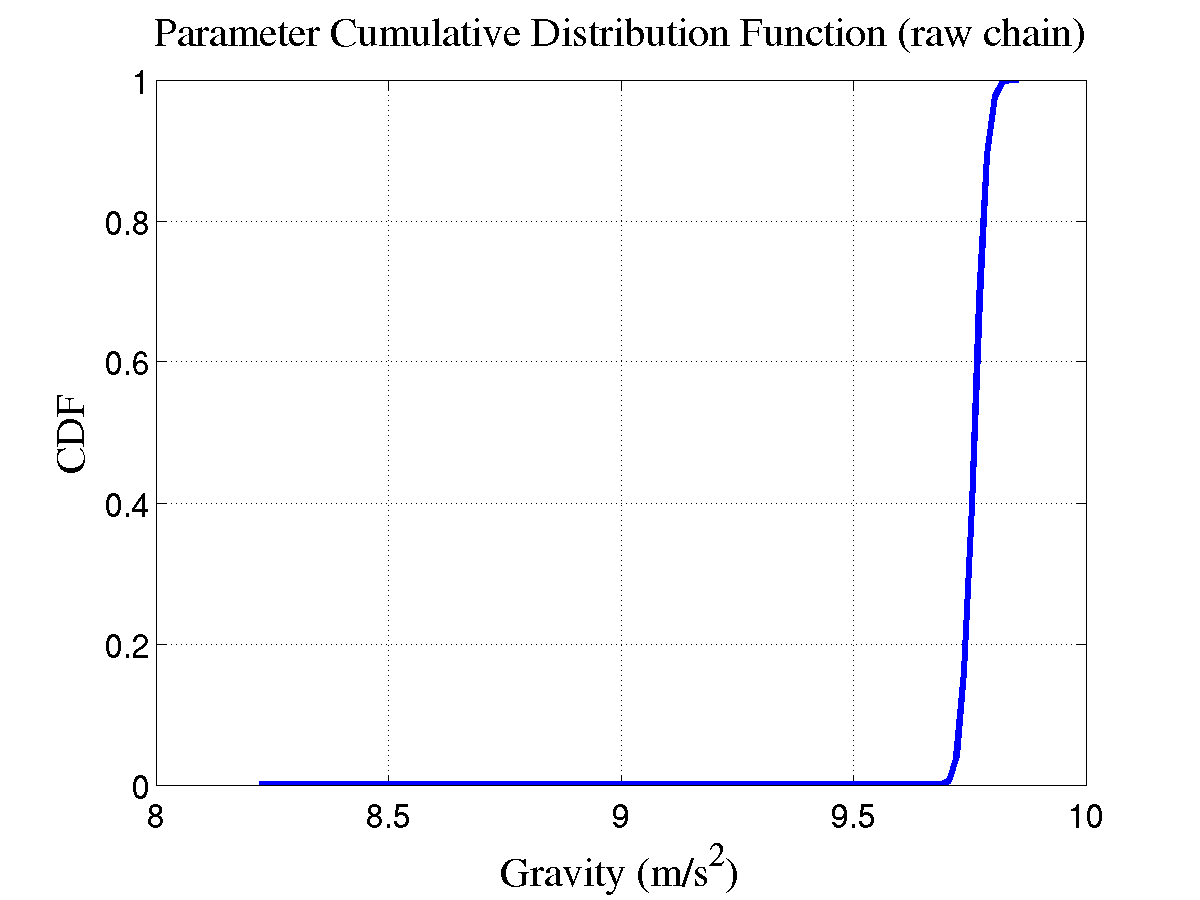
\includegraphics[scale=0.35]{figs/sip_gravity_cdf_raw.png}\label{fig:sip_gravity_cdf_raw}}
\subfigure[Filtered chain]{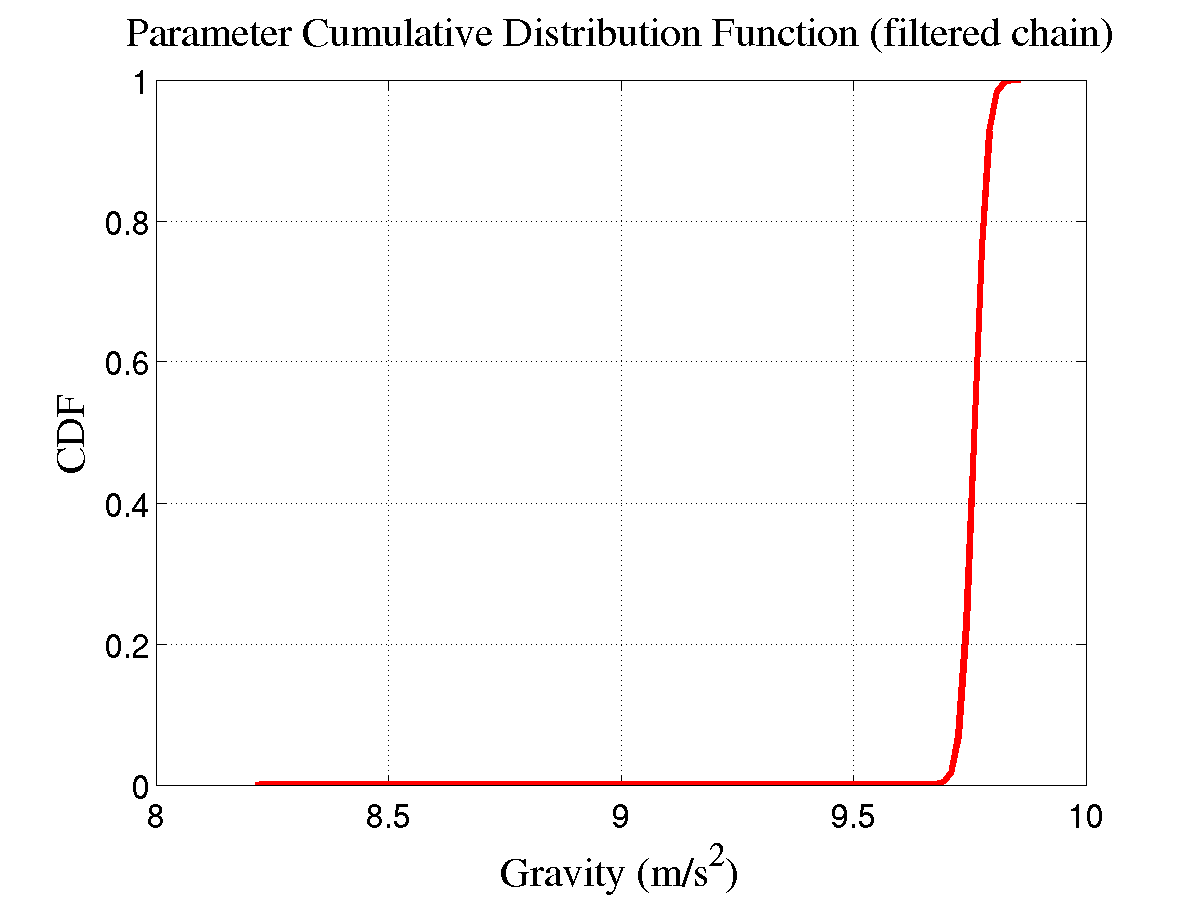
\includegraphics[scale=0.35]{figs/sip_gravity_cdf_filt.png}\label{fig:sip_gravity_cdf_filtered}}
\vspace*{-10pt}
\caption{Cumulative Distribution Function. }
\end{figure}

\paragraph{Autocorrelation Plots}\

The code presented in Listing \ref{matlab:autocorr} uses matlab function \verb+autocorr+ to generate Figure \ref{fig:sip_gravity_autocorrelation_raw_filt}
which presents the autocorrelation of the parameter $g$ in both cases: raw and filtered chain.

\begin{lstlisting}[label=matlab:autocorr,caption={Matlab code for the autocorrelation plots.}]
% inside Matlab
>> sip_gravity_raw_chain
>> sip_gravity_filtered_chain
>> nlags=10;
>> [ACF_raw,lags,bounds]= autocorr(ip_mh_rawChain_unified, nlags, 0);
>> [ACF_filt,lags,bounds]=autocorr(ip_mh_filtChain_unified,nlags, 0);
>> plot(lags,ACF_raw,'bo-',lags,ACF_filt,'r*-','linewidth',3);
>> ylabel('Autocorrelation for \theta=g','fontsize',20);
>> xlabel('Lag','fontsize',20);
>> title('Parameter Autocorrelation','fontsize',20);
>> grid on;
>> h=legend('raw chain','filtered chain','location','northeast');
>> set(h,'fontsize',16);
\end{lstlisting}

\begin{figure}[htpb]
\centering
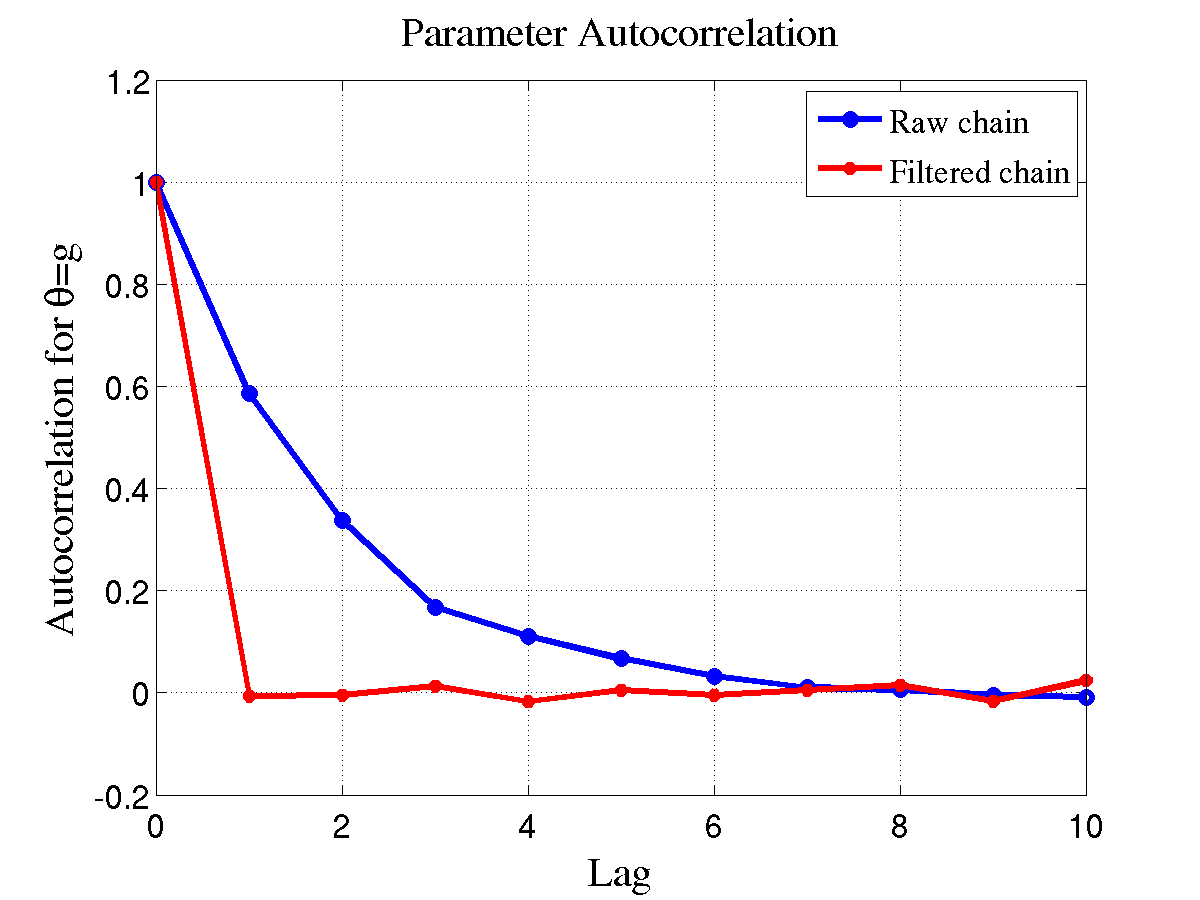
\includegraphics[scale=0.35]{figs/sip_gravity_autocorrelation_raw_filt.png}
\vspace{-8pt}
\caption{
Autocorrelation plots. }
\label{fig:sip_gravity_autocorrelation_raw_filt}
\end{figure}

\paragraph{Covariance and Correlation Matrices}\

Matlab function \verb+cov+ calculates the covariance matrix for a data matrix (where each column represents a separate quantity), and \verb+corr+ calculates the correlation matrix.
Since our statistical inverse problem has only one parameter (the acceleration $g$ due to gravity), both covariance and correlation matrices have dimension $1 \times 1$, i.e., they are scalars.

\begin{lstlisting}[label=matlab:cov_matrix,caption={Matlab code for finding the covariance matrix.}]
% inside Matlab
>> sip_gravity_raw_chain;
>> cov_matrix_g = cov(ip_mh_rawChain_unified)
   
cov_matrix_g =

   6.8709e-04
>> corr_matrix_g = corr(ip_mh_rawChain_unified)

corr_matrix_g =

     1
>>
\end{lstlisting}


\subsubsection{Statistical Forward Problem}


\paragraph{Chain Plots} \

It is quite simple to plot, using Matlab, the chain of positions generated by the Monte Carlo algorithm implemented within QUESO and called during the solution of the statistical forward problem. 
%The sequence of Matlab commands presented in Listing \ref{matlab:chain_qoi} generates the graphic depicted in Figure~\ref{fig:sfp_gravity_chain}. 

\begin{lstlisting}[label=matlab:chain_qoi,caption={Matlab code for the chain plot.}]
% inside Matlab
>> sfp_gravity_qoi_seq.m
>> plot(fp_mc_QoiSeq_unified);
>> ylabel('QoI','fontsize',20);
>> xlabel('Number of positions','fontsize',20);
>> title('MC Chain Positions','fontsize',20);
\end{lstlisting}

\begin{figure}[htb]
\centering 
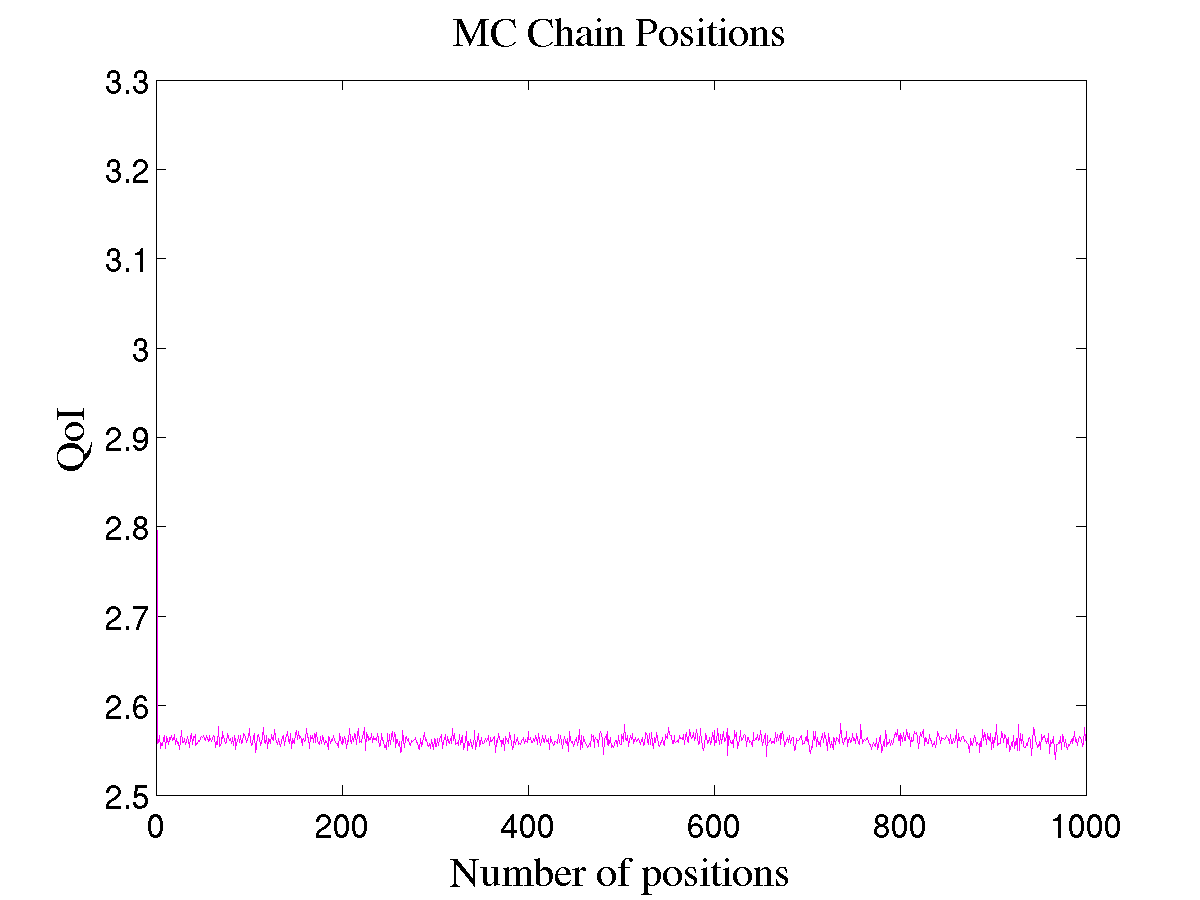
\includegraphics[scale=0.35]{figs/sfp_gravity_chain_pos.png}
\vspace*{-10pt}
\caption{MC chain positions for the QoI.}
\label{fig:sfp_gravity_chain}
\end{figure}

\paragraph{Histogram Plots} \

In order to plot a histogram of the QoI, you may use the pre-defined Matlab function \verb+hist+.
%The Matlab code presented in Listing \ref{matlab:hist_qoi} below shows how to create the Figure~\ref{fig:sfp_gravity_hist}.
%
\begin{lstlisting}[label=matlab:hist_qoi,caption={Matlab code for the QoI histogram plot.}]
>> sfp_gravity_qoi_seq.m
>> nbins=100;
>> hist(fp_mc_QoiSeq_unified);
>> title('QoI Histogram','fontsize',20);
>> xlabel('Distance traveled (m)','fontsize',20);
>> ylabel('Frequency','fontsize',20);
>> grid on;
\end{lstlisting}

\begin{figure}[htb]
\centering 
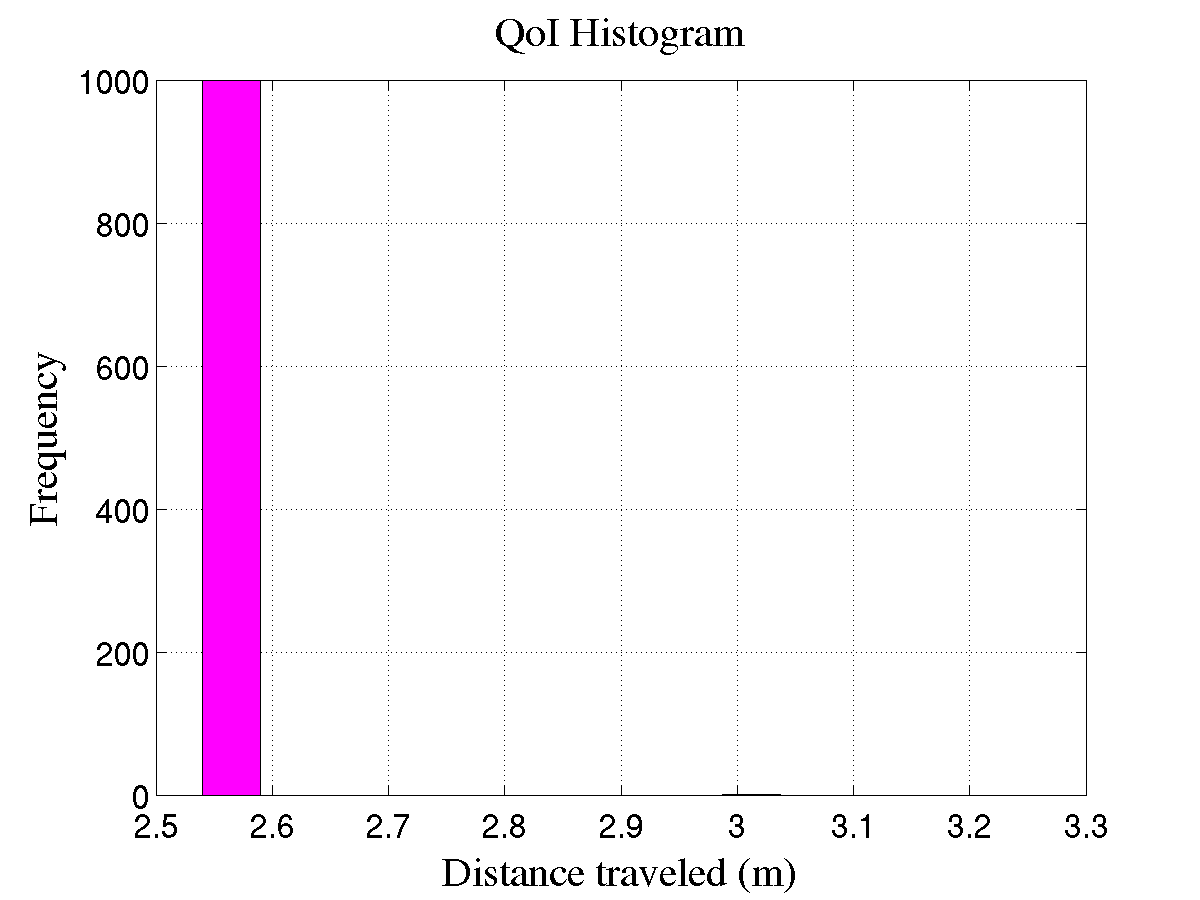
\includegraphics[scale=0.35]{figs/sfp_gravity_hist.png}
\vspace{-10pt}
\caption{Histogram of QoI $=d$.}
\label{fig:sfp_gravity_hist}
\end{figure}

\paragraph{KDE Plots} \

Matlab function \verb+ksdensity+ (Kernel smoothing density estimate) together with the option \verb+'pdf'+ may be used for plotting the KDE of the he QoI.
\begin{lstlisting}[label=matlab:kde_qoi,caption={Matlab code for the QoI KDE plot.}]
% inside Matlab
>> sfp_gravity_qoi_seq.m
>> [f,xi] = ksdensity(fp_mc_QoiSeq_unified,'function','pdf');
>> plot(xi,f,'-b','linewidth',3)
>> title('QoI Kernel Density Estimation ','fontsize',20);
>> xlabel('Distance traveled (m)','fontsize',20);
>> ylabel('KDE','fontsize',20);
>> grid on;
\end{lstlisting}

\begin{figure}[p]
\centering 
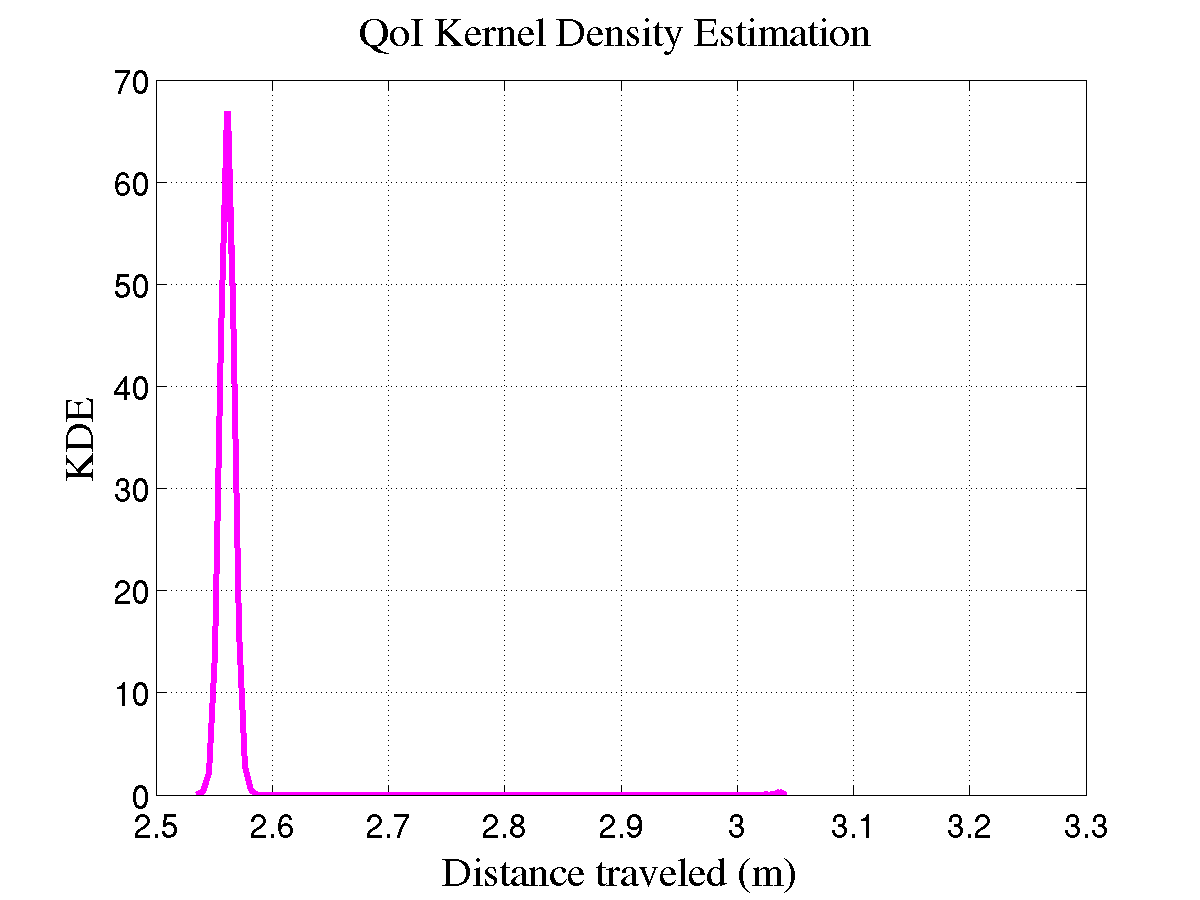
\includegraphics[scale=0.35]{figs/sfp_gravity_kde.png}
\vspace*{-10pt}
\caption{Kernel Density Estimation.}
\label{fig:sfp_gravity_kde}
\end{figure}

\paragraph{CDF Plots} \

Matlab function \verb+ksdensity+ (Kernel smoothing density estimate) with \verb+'cdf'+ option may also be used for plotting the Cumulative Distribution Function of the QoI.

\begin{lstlisting}[label=matlab:cdf_qoi,caption={Matlab code for the QoI CDF plot.}]
% inside Matlab
>> sfp_gravity_qoi_seq.m
>> [f,xi] = ksdensity(fp_mc_QoiSeq_unified,'function','cdf');
>> plot(xi,f,'-b','linewidth',3)
>> title('QoI Cumulative Distribution Function ','fontsize',20);
>> xlabel('Distance traveled (m)','fontsize',20);
>> ylabel('CDF','fontsize',20);
>> grid on;
\end{lstlisting}

\begin{figure}[p]
\centering 
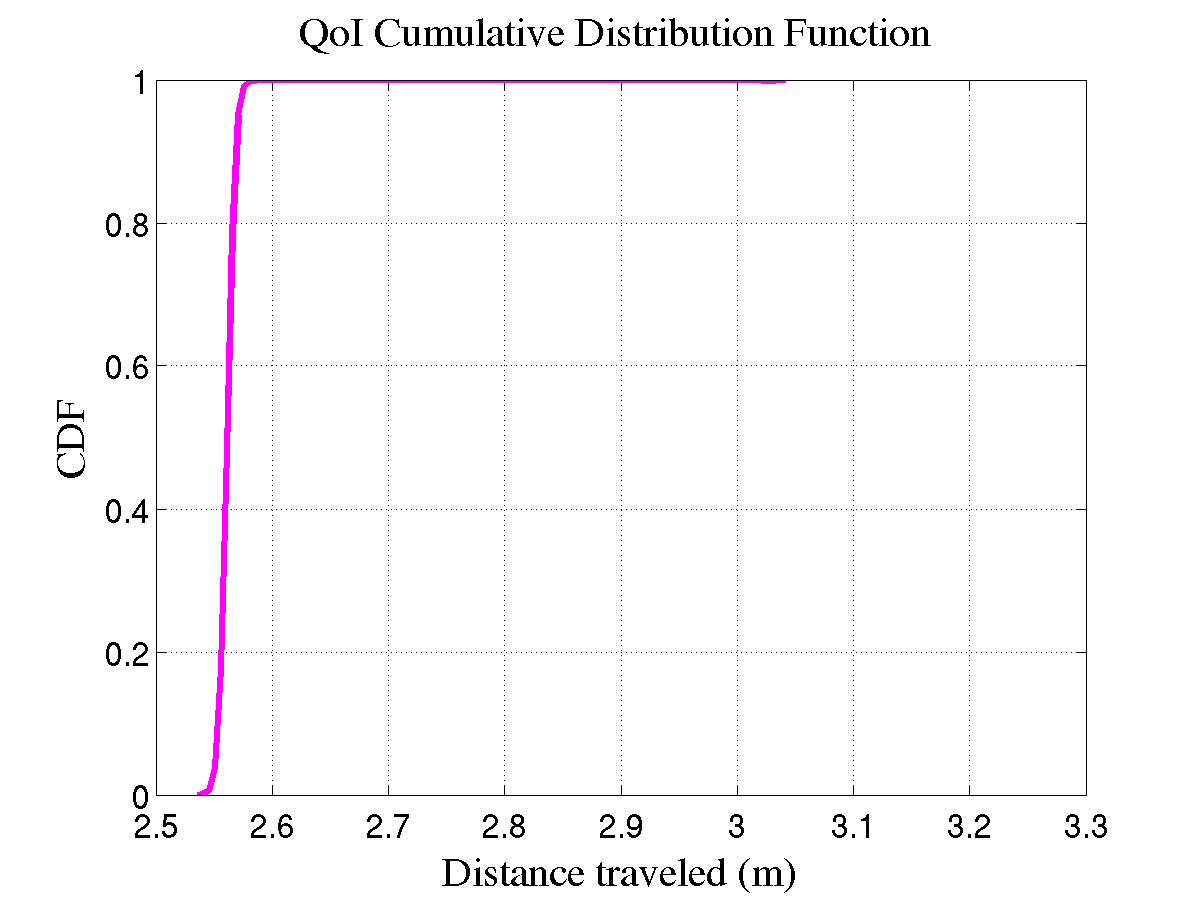
\includegraphics[scale=0.35]{figs/sfp_gravity_cdf.png}
\vspace*{-10pt}
\caption{Cumulative Distribution Function.}
\label{fig:sfp_gravity_cdf}
\end{figure}

\paragraph{Autocorrelation Plots} \

The code presented in Listing \ref{matlab:autocorr_qoi} uses Matlab function \verb+autocorr+ to generate Figure \ref{fig:sfp_gravity_autocorrelation},
which presents the autocorrelation of the QoI $d$.

\begin{lstlisting}[label=matlab:autocorr_qoi,caption={Matlab code for the QoI autocorrelation plot.}]
% inside Matlab
>> sfp_gravity_qoi_seq.m
>> nlags=10;
>> [ACF, lags, bounds] = autocorr(fp_mc_QoiSeq_unified, nlags, 0);
>> plot(lags,ACF,'bo-','linewidth',3);
>> ylabel('Autocorrelation for QoI = d','fontsize',20);
>> xlabel('Lag','fontsize',20);
>> title('QoI Autocorrelation','fontsize',20);
>> grid on;
\end{lstlisting}

\begin{figure}[p]
\centering
\includegraphics[scale=0.35]{figs/sfp_gravity_autocorrelation.png}
\vspace*{-10pt}
\caption{Autocorrelation plot.}
\label{fig:sfp_gravity_autocorrelation}
\end{figure}

\paragraph{Covariance and Correlation Matrices} \

For a matrix input \verb+X+, where each row is an observation, and each column is a variable, the Matlab function \verb+cov(X)+ may be used to calculate the covariance matrix.
%The command \verb+diag(cov(X))+ is a vector of variances for each column, and, therefore, \verb+sqrt(diag(cov(X)))+ is a vector of standard deviations.  

Thus,  in order to calculated the covariance matrix between the parameter and the quantity of interest sequences generated by Monte Carlo sampler with QUESO,
one may simply define \verb+X=[fp_mc_ParamSeq_unified fp_mc_QoiSeq_unified]+.
The code presented in Listing \ref{matlab:cov_pqoi} shows the usage of Matlab commands for finding such the matrix.

\begin{lstlisting}[label=matlab:cov_pqoi,caption={Matlab code for the matrix of covariance between parameter $g$ and QoI $d$.}]
% inside Matlab
>> sfp_gravity_qoi_seq;
>> sfp_gravity_p_seq;
>> X=[fp_mc_ParamSeq_unified fp_mc_QoiSeq_unified];
>> cov_p_QoI = cov(X)

cov_p_QoI =
	  [ 2.826e-03 	-8.555e-04 ] 
	  [-8.555e-04 	 2.599e-04 ]

\end{lstlisting}

Analogously, the Matlab function \verb+corrcoef(X)+ returns a matrix of correlation coefficients calculated from an input matrix \verb+X+ whose rows are observations and whose columns are variables.
In order to calculated the correlation matrix between the parameter and the QoI sequences, one may simply define \verb+X=[fp_mc_ParamSeq_unified fp_mc_QoiSeq_unified]+.
% The matrix R = corrcoef(X) is related to the covariance matrix C = cov(X) b

\begin{lstlisting}[label=matlab:corr_param_qoi,caption={Matlab code for the matrix of correlation between parameter $g$ and quantity of interest $d$.}]
% inside Matlab
>> sfp_gravity_qoi_seq;
>> sfp_gravity_p_seq;
>> X=[fp_mc_ParamSeq_unified fp_mc_QoiSeq_unified];
>> corr_p_QoI = corrcoef(X)

corr_p_QoI =
	  [ 1.000e+00 	-9.981e-01 ] 
	  [-9.981e-01 	 1.000e+00 ]
>>
\end{lstlisting}




\section{\texttt{validationCycle}}\label{sec:example_tga}

This is the last and more complex of all \Queso{} examples. 
In this example, we numerically solve a statistical inverse problem related to a thermogravimetric experiment, where a material sample has its mass measured while loosing it through a controlled heating process. 

Given a simple mass evolution model that has a temperature profile and material
properties as input parameters, and given thermogravimetric measurements with
prescribed variances, the statistical inverse problems ask for the
specification of the random variables that represent the unknown material
properties. We compute probability density functions with the Bayesian approach
and compute sets of realizations through the Metropolis-Hastings algorithm with
delayed rejection.
% DRAM Markov chain algorithm.
%Once the random variables are computed, they become input parameters on statistical forward problems,
%which ask for the statistical prediction of the sample mass evolution under a specified temperature profile.
%We solve the statistical forward problems with the Monte Carlo algorithm.

We qualitatively analyze the sensitivity of the solutions with respect to
problem characteristics, namely ``amount'' of data and ``quality'' of data, and
also with respect to algorithm options, namely chain initial position, number
of delayed rejections
%, covariance matrix adaptivity
and chain size.




\subsection{Thermogravimetric Experiments and a Simple Model}

Suppose a given material sample of initial mass $m_0$ and at initial temperature $T_0$ is heated with constant heating rate $\beta$ (K/min). Heating is maintained until the sample fully ablates (decomposes). The sample mass $m(T)$ is measured at temperatures $T>T_0$.
Let $w(T)~=~m(T)/m_0$ denote the mass fraction.

% 
% A material sample with initial mass $m_0$ and at initial temperature $T_0$ is heated
% with constant heating rate $\beta$ (K/min) until it fully decomposes.
% Let $w(T)=m(T)/m_0$ denote the mass fraction.
\begin{figure}[!ht]
\centering
\includegraphics[scale=0.4]{figs/tga_experiment_data.png}
\vspace*{-8pt}
\caption{Mass fraction decay over temperature given different heating rates. Data from J. A. Conesa, R. F. Marcilla and J. A. Caballero, ``Thermogravimetric studies on the thermal decomposition of polyethylenes'', {\it J. Anal. Appl. Pyrolysis}, 36(1):1-15, 1996}
\label{fig:tga-exp-data}
\end{figure}


It is convenient to transform the kinetic equation to a \emph{per unit temperature}
form by dividing through by $\beta$. Thus, a simple approach to
the simulation of a thermogravimetric phenomenon consists on modeling the
sample as a homogeneous material of scalar properties $A>0$ and $E>0$ whose
relative mass $w$ obeys the following initial value ordinal differential
equation problem:
\begin{equation}\label{eq:tga-model}
\left\{
\begin{array}{rcll}
{\displaystyle \frac{dw}{dt} } & = & -\dfrac{A w}{\beta} \exp\left(-\frac{E}{RT}\right), & t \geqslant 0,\\
& & \\
w(0) & = & 1, &
\end{array}
\right.
\end{equation}
where the kinetic parameters $A$ and $E$ are referred to, respectively, as pre-exponential factor (min$^{-1}$) and activation energy (J/mol).


In this combined SIP--SFP, we  calibrate both model parameters $A$ and $E$ given the mathematical model in Equation \eqref{eq:tga-model} and experimental data (Section \ref{sec:tga-data}). Then the inferred values for $A$ and $E$ are then used for uncertainty propagation on the remaining mass fraction at time $t=3.9$ s when $\beta=250$ K/min, i.e., our quantity of interest is $w(t=3.9)$. 

\subsection{Statistical Inverse Problem}\label{sec:tga-sip}

%
Let $\mathbf{m}=(A,E)$ be the vector of model parameters and $M=\mathbb{R}_{+}^{2}$ be the space of model parameters.
Let
$V_T$ denote the space of functions $f:\mathbb{R}_{+}\rightarrow\mathbb{R}_{+}$ that are weakly differentiable.
$V_T$ will be the space of temperature profiles.
Finally, let
$V_w$ denote the space of functions $f:\mathbb{R}_{+}\rightarrow[0,1]$ that are weakly differentiable.
$V_w$ will be the space of relative mass evolutions.
We will denote by
\begin{equation*}
w(\mathbf{m},T)\in V_w
\end{equation*}
the solution of Equation \eqref{eq:tga-model} for given $\mathbf{m}\in M$ and $T\in V_T$.


% 
% This model can be easily generalized to a sample composed of $N_{\text{mat}}\geqslant 1$ materials. We refer to \cite{eep_ices_rep1} for details.

\subsubsection{Misfit Functions $\mathcal{F}(\mathbf{m})$}

Let
$V_S$ denote the space of all functions $f:\mathbb{R}_{+}\rightarrow\mathbb{R}_{+}$ that are square-Lebesgue-integrable
over any finite interval.
$V_S$ will be the space of misfit weight functions.
Let
$V_{\sigma}$ denote the space of all functions $f:\mathbb{R}_{+}\rightarrow\mathbb{R}_+^{*}$ such that $1/f$ is square-Lebesgue-integrable
over any finite interval.
$V_{\sigma}$ will be the space of variance functions.

Given a reference relative mass evolution function $\text{$d$}\in V_w$,
a temperature profile $T\in V_T$,
and some $t_{_{\text{F}}}>0$,
let $\mathcal{F}:M\rightarrow\mathbb{R}$ be the functional defined by
\begin{equation*}
\mathcal{F}(\mathbf{m}) = \int_{0}^{t_{_{\text{F}}}}~\left\{[w(\mathbf{m},T)](t)-\text{$d$}(t)\right\}^2\cdot S(t)~dt,
\end{equation*}
or simply
\begin{equation}\label{eq-F}
\mathcal{F}(\mathbf{m}) = \int_{0}^{t_{_{\text{F}}}}~(w-d)^2\cdot S~dt.
\end{equation}


The functional \eqref{eq-F} is general enough for our studies, since it can properly describe
not only the case where one has continuous measurements $\text{$d$}$,
but also the case of a finite set of $N_{\text{meas}}$ discrete measurements $0\leqslant d_j\leqslant 1$,
$1\leqslant i\leqslant N_{\text{meas}}$ at instants $0\leqslant t_1 < t_2 < \ldots < t_{N_{\text{meas}}}$.

In the case of continuous measurements, for instance, one can set
\begin{equation*}
\mathcal{F}_1(\mathbf{m}) = \int_{0}^{t_{_{\text{F}}}}~\left\{[w(\mathbf{m},T)](t)-\text{$d$}(t)\right\}^2\cdot\frac{1}{\sigma^2(t)}~dt,
\end{equation*}
for some given variance function $\sigma^2\in V_S$ satisfying $\sigma(t)>0$ for all $t\geqslant 0$.

On the other hand, when measurements are discrete and a corresponding finite set of variances $\sigma_j^2>0,~j=1,2,\ldots,N_{\text{meas}}$ is given, one can set
\begin{equation*}
\mathcal{F}_2(\mathbf{m}) = \int_0^{t_{_F}}~\{[w(\mathbf{m},T)](t)-\hat{d}(t)\}^2\cdot\left[\sum_{j=1}^{N_{\text{meas}}}\frac{\delta(t-t_j)}{{\hat{\sigma}}^2(t)}\right]~dt,
\end{equation*}
where
$\hat{d}\in V_w$ and $\hat{\sigma}\in V_{\sigma}$ are any functions satisfying
$\hat{d}(t_j)=d_j$ and $\hat{\sigma}(t_j)=\sigma_j$, $j=1,2,\ldots,N_{\text{meas}}$,
in which case the functional simply becomes
\begin{equation*}
\mathcal{F}_2(\mathbf{m}) = \sum_{j=1}^{N_{\text{meas}}}~\frac{\{[w(\mathbf{m},T)](t_j)-d_j\}^2}{\sigma_j^2},
\end{equation*}
assuming, without loss of generality, that $t_{_F}\geqslant t_{N_{\text{meas}}}$.

\subsubsection{Bayesian Approach: Prior RV, Likelihood and Posterior RV}


In \underline{deterministic} inverse problems treat the unknown parameters as scalars or vectors and the goal is
the calculation of their best values according to a given criteria, usually least squares, e.g. solving the unconstrained optimization problem
\begin{equation}\label{eq-unconstrained-min}
\underset{\mathbf{m}\in M}{\text{min}}~\mathcal{F}(\mathbf{m}).
\end{equation}

In \underline{statistical} inverse problems, the unknown parameters are treated
as random variables (RVs) and the goal is the specification of their
probability density functions (PDFs)~\cite{KaSo05}.




Applying the Bayesian approach
\begin{equation*}
\pi_{\text{posterior}}(\mathbf{m})\propto \pi_{\text{prior}}(\mathbf{m})\cdot\pi_{\text{likelihood}}(\mathbf{m})
\end{equation*}
we have that for the TGA SIP, the prior distribution and the likelihood are, respectively:
\begin{equation*}
\pi_{\text{prior}}(\mathbf{m}) \propto e^{-\frac{1}{2}V(\mathbf{m})}\quad\text{and}\quad
%
\pi_{\text{likelihood}}(\mathbf{m}) \propto e^{-\frac{1}{2}\mathcal{F}(\mathbf{m})}.
\end{equation*}


Thus, we chose parameters $(A,E)$ to have joint uniform prior PDF over the open
square domain, i.e.:
$$\pi_{\text{prior}}=\mathcal{U}((1.0\times 10^{10},5.0\times 10^{11})\times (4.0\times 10^{5},6.0\times 10^{5})).$$



\subsubsection{Data from experiments}\label{sec:tga-data}

Table \ref{table:data-tga} presents the data collected in the TGA experiment. 

\begin{table}[htb]
\begin{center}
\begin{tabular}{cllc}
\toprule
Observation   & Temperature     & Relative mass             & Variance \\
index ``$i$'' & $T_i$ (K)       & $m^*_{\text{obs},i}$ (\%) & $V_i$    \\
\midrule
\midrule
 1            & $\quad$ 673.034 & $\quad$ 96.5855    & 0.1      \\
 2            & $\quad$ 682.003 & $\quad$ 95.1549    & 0.1      \\
 3            & $\quad$ 690.985 & $\quad$ 92.5048    & 0.1      \\
 4            & $\quad$ 699.979 & $\quad$ 88.6353    & 0.1      \\
 5            & $\quad$ 708.989 & $\quad$ 83.0585    & 0.1      \\
 6            & $\quad$ 718.02  & $\quad$ 75.5306    & 0.1      \\
 7            & $\quad$ 727.089 & $\quad$ 64.1003    & 0.1      \\
 8            & $\quad$ 735.96  & $\quad$ 47.5474    & 0.1      \\
 9            & $\quad$ 744.904 & $\quad$ 23.6777    & 0.1      \\
 10           & $\quad$ 754.062 & $\quad$ 03.2234    & 0.1      \\
 11           & $\quad$ 763.049 & $\quad$ 00.0855448 & 0.1      \\
\bottomrule
\end{tabular}
\vspace{-.2cm}
\caption{Experimental data.}\label{table:data-tga}
\end{center}
\end{table}

\subsection{Statistical Forward Problem}\label{sec:tga-sfp}

In spacecraft design, ablation is used to both cool and protect mechanical parts and/or payloads that would otherwise be damaged by extremely high temperatures. Two principal applications are heat shields for spacecraft entering a planetary atmosphere from space and cooling of rocket engine nozzles~\cite{wiki:ablation}. 

Suppose that an object about to re-enter the Earth atmosphere has a thermal
protection layer (shield) of composition of the same sample material described
in Section \ref{sec:tga-sip}. Also, as the object re-enters the atmosphere, its
shield loses mass according to Equation \eqref{eq:tga-model}.  The initial
sample temperature is $T_0=0.1$ K and it is then heated with constant rate
$\beta=5$ K/m.
% We are interested in answering a few questions:
% \begin{enumerate}
%  \item At scenario $\beta=250$ K/min, what is the remaining mass fraction at time $t=3.9$ s, i.e. $$w(t=3.9s)?$$
%  \item Supposing that a failure occurs when the remaining mass fraction is smaller than 20\%, what is the probability of failure at time $t=3.9$ s, i.e. $$P(w(t=3.9s)<0.2)?$$
%  \item  Supposing that the probability of failure is $\leq 5\%$, what is the margin in the prediction of the probability of failure?
% \end{enumerate}

We are interested in answering the following question: at scenario $\beta=250$
K/min, what is the remaining mass fraction at time $t=3.9$ s? In other words,
the quantity of interest is $w(t=3.9s)$.



% \todo{Suppose also that, under such conditions, our quantity of interest (QoI) is the time necessary to the sample to ablate 75\% of its mass, denoted by $t_\text{0.25}$ (s). In other words, we are interested in estimate how long it takes for $w=0.25$, or}
% \begin{equation}
%  \text{Find } t_\text{0.25} \text{ such as } w(t_\text{0.25} )=0.25
% \end{equation}

\subsubsection{The Input RV, QoI Function and Output RV}


The input random variables for this SFP are the inferred parameters $A$ and $E$ which are the solution (posterior PDF) of the inverse problem described in Section \ref{sec:tga-sip}. The output random variable for this example is the remaining mass fraction at 3.9 s, i.e. $w(t=3.9)$. Note that, since there is uncertainty in the parameters $A$ and $E$ (both given as PDFs), one can expect that this uncertainty will be propagated to $w(t=3.9)$, which will also be given as a PDF. Finally, the QoI function for $w$ is the solution of the Equation \eqref{eq:tga-model} evaluated when $t=3.9$ s, which is calculated using numerical integration with adjustable and acceptable time-stepping using GSL function \verb+gsl_odeiv_evolve_apply+\footnote{\url{http://www.gnu.org/software/gsl/manual/html_node/Evolution.html\#index-gsl_005fodeiv2_005fevolve_005fapply}}. 

\subsection{Running the Example}\label{sec:tga-run}

To run the executable provided (available after QUESO installation), and generate figures for the chains, PDFs, CDFs, etc., enter the following commands:
\begin{lstlisting}[label={},caption={}]
$ cd $HOME/LIBRARIES/QUESO-0.50.0/examples/validationCycle
$ rm outputData/*
$ ./exTgaValidationCycle_gsl tagCycle.inp    
$ matlab
   $ tga_cycle_plot.m     # inside matlab
   $ exit                 # inside matlab
$ ls -l outputData/*.png
  cal_parameter1_prior.png                cal_parameter2_prior.png                
  cal_val_parameter1_PDF.png              cal_val_parameter2_PDF.png              
  cal_val_parameter1_CDF.png              cal_val_parameter2_CDF.png              
  cal_val_parameter1_autocorr.png         cal_val_parameter2_autocorr.png
  cal_val_QoI_CDF.png                     cal_val_QoI_PDF.png
  cal_val_QoI_autocorrelation.png            
\end{lstlisting}
% cal_val_QoI_CDF_model_confidence_full.png
% cal_val_QoI_CDF_model_confidence_zoom.png


As a result, the user should have created several of PNG figures containing marginal posterior PDF, chain positions of the parameters and the QoI, histogram, cumulative density distribution and autocorrelation. The name of the figure files have been chosen to be informative, as shown in the Listing above.



\subsection{TGA Example Code}\label{sec:code-tga}



The program example given in this paper is compatible with version 0.47.1 of QUESO.
The source code for the example is composed of 5 files:
 \texttt{exTgaValidationCycle\_gsl.C} (Listing \ref{code:tga-main-c}),
 \texttt{exTgaValidationCycle\_appl.h} (Listing \ref{code:tga-appl-h}), 
 \texttt{exTgaValidationCycle\_likelihood.h}  (Listing \ref{code:tga-like-h}) and 
\texttt{exTgaValidationCycle\_qoi.C} (Listing \ref{code:tga-qoi-h}).



\lstinputlisting[caption=File \texttt{exTgaValidationCycle\_gsl.C}., label={code:tga-main-c}, linerange={28-1000}]{../../examples/validationCycle/src/exTgaValidationCycle_gsl.C}

\lstinputlisting[caption=File \texttt{exTgaValidationCycle\_appl.h}., label={code:tga-appl-h}, linerange={27-1000}]{../../examples/validationCycle/src/exTgaValidationCycle_appl.h}

\lstinputlisting[caption=File \texttt{exTgaValidationCycle\_likelihood.h.}, label={code:tga-like-h}, linerange={27-1000}]{../../examples/validationCycle/src/exTgaValidationCycle_likelihood.h}

\lstinputlisting[caption=File \texttt{exTgaValidationCycle\_qoi.h}., label={code:tga-qoi-h}, linerange={27-1000}]{../../examples/validationCycle/src/exTgaValidationCycle_qoi.h}




\subsection{Input File}\label{sec:tga-input-file}

The input file used with this TGA SIP--SFP QUESO provides QUESO with options
for its environments, and for both  MCMC and Monte-Carlo algorithms. It is
displayed in Listing~\ref{code:tga-input-file}.


\lstinputlisting[caption={File name \texttt{tgaCycle.inp} with options for QUESO library used in application code (Listings \ref{code:tga-main-c}-\ref{code:tga-like-h}})., 
label={code:tga-input-file},]{../../examples/validationCycle/tests/test_2012_11_15/tgaCycle.inp}



\subsection{Data Post-Processing and Visualization}\label{sec:tga-results}


According to the specifications of the input file in Listing~\ref{code:tga-input-file}, both a folder named \verb+outputData+ and a the following files should be generated:
\begin{verbatim}
file_cal_ip_raw.m        file_val_ip_raw.m        
file_cal_ip_raw_sub0.m   file_val_ip_raw_sub0.m
file_cal_fp_qoi2.m       file_val_fp_qoi2.m      
file_cal_fp_qoi2_sub0.m  file_val_fp_qoi2_sub0.m     
tgaCalOutput_sub0.m      tgaValOutput_sub0.m
display_sub0.txt    
\end{verbatim}


The sequence of Matlab commands is identical to the ones presented in Sections
\ref{sec:sip-results}, \ref{sec:sfp-results} and \ref{sec:gravity-results};
therefore, are omitted here. The reader is invited to explore the Matlab file
\texttt{tga\_cycle\_plot.m}  
%\texttt{validationCycle/tests/test\_2012\_11\_15/tga\_cycle\_plot.m} 
for details of how the figures have been generated.

\subsubsection{KDE Plots of Parameters}
Matlab function \verb+ksdensity+ (Kernel smoothing density estimate) together
with the option `\verb+pdf+' may be used to estimate the KDE of the parameters,
as illustrated in Figure \ref{fig:tga_ip_pdf}.
% \begin{figure}[htb]
% \centering 
% \subfloat{\includegraphics[scale=0.40]{figs/cal_parameter1_prior.png}}
% \subfloat{\includegraphics[scale=0.40]{figs/cal_parameter2_prior.png}}
% \vspace*{-10pt}
% \caption{Prior distributions of parameters $A$ and $E$.}
% \end{figure}
%
\begin{figure}[htpb]
\centering 
\subfloat{\includegraphics[scale=0.3]{figs/cal_val_parameter1_PDF.png}}
\subfloat{\includegraphics[scale=0.3]{figs/cal_val_parameter2_PDF.png}}
\vspace*{-10pt}
\caption{Posterior distributions of parameters $A$ and $E$.}
\label{fig:tga_ip_pdf}
\end{figure}



\subsubsection{CDF Plots of Parameters}

Matlab function \verb+ksdensity+ with \verb+'cdf'+ option may also be used for plotting the Cumulative Distribution Function of each one of the parameters, as illustrated in Figure \ref{fig:tga_ip_cdf}.
%
\begin{figure}[htpb]
\centering 
\subfloat{\includegraphics[scale=0.3]{figs/cal_val_parameter1_CDF.png}}
\subfloat{\includegraphics[scale=0.3]{figs/cal_val_parameter2_CDF.png}}
\vspace*{-10pt}
\caption{Cumulative density functions of parameters $A$ and $E$.}
\label{fig:tga_ip_cdf}
\end{figure}



\subsubsection{Autocorrelation Plots of Parameters}

Figure \ref{fig:tga_ip_autocorrelation_param} presents the autocorrelation of the parameters $A$ and $E$ in both cases: calibration and validation stages.

\begin{figure}[p]
\centering 
\subfloat{\includegraphics[scale=0.3]{figs/cal_val_parameter1_autocorrelation.png}}
\subfloat{\includegraphics[scale=0.3]{figs/cal_val_parameter2_autocorrelation.png}}
\vspace*{-10pt}
\caption{Autocorrelation of parameters $A$ and $E$ (filtered chain).}
\label{fig:tga_ip_autocorrelation_param}
\end{figure}


\subsubsection{KDE, CDF and Autocorrelation Plots of QoI}
Figures \ref{fig:tga_pdf_qoi}  and \ref{fig:tga_cdf_qoi} present PDF and CDF of QoI, respectively and Figure \ref{fig:tga_autocorrelation_qoi} presents its autocorrelation.


\begin{figure}[p]
\centering 
\subfloat[QoI PDF]{\includegraphics[scale=0.3]{figs/cal_val_QoI_PDF.png}\label{fig:tga_pdf_qoi}}
\subfloat[QoI CDF]{\includegraphics[scale=0.3]{figs/cal_val_QoI_CDF.png}\label{fig:tga_cdf_qoi}}
\vspace*{-10pt}
\caption{QoI PDF and CDF, during calibration and validation stages.}
\end{figure}


%
% \begin{figure}[htb]
% \centering
% \includegraphics[scale=0.35]{figs/cal_val_QoI_CDF.png}
% \vspace*{-10pt}
% \caption{QoI CDF, during calibration and validation stages.}
% \label{fig:tga_cdf_qoi}
% \end{figure}

\begin{figure}[p]
\centering 
\includegraphics[scale=0.3]{figs/cal_val_QoI_autocorrelation}
\vspace*{-10pt}
\caption{QoI autocorrelation.}
\label{fig:tga_autocorrelation_qoi}
\end{figure}


\section{\texttt{modal}}\label{sec:example_modal}


This example presents a combination of two statistical inverse problems in one. 
It presents the capability of the Multilevel method in sampling from a target distribution that has either one or two modes (distinct peaks). The random variable of interest has three parameters, i.e., $\bv{\theta}=(\theta_1,\theta_2, \sigma^2) \in \mathbb{R}^3$, where the third parameter may be seen as variation.

The example also it gives the user the opportunity to chose either one single type of prior distribution, uniform, for the three components of the random variable, or two different priors: a uniform and a beta distribution.

Choosing between a one-mode or a two-mode target distribution is done at execution level, as presented in the following code line:

\begin{lstlisting}[label={},caption={}]
$ cd $HOME/LIBRARIES/QUESO-0.50.0/
$ cd examples/modal
$ rm outputData/*
$ ./modal_gsl example.inp <num_of_nodes>
\end{lstlisting}
where \verb+<num_of_nodes>+ is either 1 or 2.
% 
% 
% This simple statistical inverse problem presents a combination of two, suppose a random variable of interest with three parameters $\bv{\theta}=(\theta_1,\theta_2, \sigma) \in \mathbb{R}^3$,  namely $\bv{\theta}:[0,3]\times[0,3]\times[0,0.3] \rightarrow\mathbb{R}$. 
% 
% 
% 
% This simple statistical inverse problem, suppose a random variable of interest with three parameters $\bv{\theta}=(\theta_1,\theta_2, \sigma) \in \mathbb{R}^3$,  namely $\bv{\theta}:[0,3]\times[0,3]\times[0,0.3] \rightarrow\mathbb{R}$. 
% 
% 
% Suppose also that the distribution we aim to sample has either one or two modes.
% 
\subsection{One-mode distribution}

In this case, the target distribution is assumed to have only one mode.
Suppose also that the random variable $\bv{\theta}$  can either have a uniform prior distribution for all its components, i.e.:
$$
% \pi_{\text{prior}}=\mathcal{U}([0,3],[0,3],[0,0.3]).
\pi_{\text{prior}}=\mathcal{U}([0,3]) \times \mathcal{U}([0,3]) \times \mathcal{U}([0,0.3]).
$$
or, the prior distribution is defined as a combination of uniform prior for $\theta_1$ and $\theta_2$, with a beta prior for $\sigma^2$:
$$
% \pi_{\text{prior}}=\mathcal{U}([0,3],[0,3],[0,0.3]).
\pi_{\text{prior}}=\mathcal{U}([0,3]) \times \mathcal{U}([0,3]) \times \mathcal{B}(\alpha,\beta), \quad \text{with} \quad \alpha=3 \quad\text{and}\quad \beta=0.09709133373799.
$$

The likelihood function is defined as follows:
\begin{equation}
\begin{split} \small
%\pi_{\text{likelihood}}(\mathbf{d}|\boldsymbol{\theta}) = 
\quad f(\D|\bv{\theta})= -\dfrac{5}{2} \log\left(2 \pi \sigma^2\right)-\dfrac{1}{2\sigma^2} &\Bigg[
 \left(10 \sqrt{10 \theta_1+20 \theta_2+10 \sqrt{\theta_1^2+4 \theta_2^2}}-72.0470\right)^2 +\\
&+\left(10 \sqrt{10 \theta_1+20 \theta_2+10 \sqrt{\theta_1^2+4 \theta_2^2}}-71.8995\right)^2 +\\
&+\left(10 \sqrt{10 \theta_1+20 \theta_2+10 \sqrt{\theta_1^2+4 \theta_2^2}}-72.2801\right)^2 +\\
&+\left(10 \sqrt{10 \theta_1+20 \theta_2+10 \sqrt{\theta_1^2+4 \theta_2^2}}-71.9421\right)^2 +\\
&+\left(10 \sqrt{10 \theta_1+20 \theta_2+10 \sqrt{\theta_1^2+4 \theta_2^2}}-72.3578\right)^2 \Bigg].
\end{split}
\end{equation}

\subsubsection{Running the One-Mode Example}
 
To run the executable provided considering a \underline{one-mode} distribution, enter the following commands:
\begin{lstlisting}[label={},caption={Running the example with a one-mode distribution.}]
$ cd $HOME/LIBRARIES/QUESO-0.50.0/
$ cd examples/modal
$ rm outputData/*
$ ./modal_gsl example.inp 1      #one mode!
$ matlab
   $  plot_modal_all_levels_1mode  # inside matlab
   $ exit                          # inside matlab
$ ls -l outputData/*.png
modal_1_mode_kde_target.png  modal_1_mode_level_1.png  modal_1_mode_level_5.png
modal_1_mode_kde_theta1.png  modal_1_mode_level_2.png  modal_1_mode_level_6.png
modal_1_mode_kde_theta2.png  modal_1_mode_level_3.png  modal_1_mode_level_7.png
modal_1_mode_kde_theta3.png  modal_1_mode_level_4.png
\end{lstlisting}

As a result, the user should have created several of PNG figures scatter plots of each one of the levels and the kernel density estimation of the parameters, for each level in the Multilevel method. The name of the figure files have been chosen to be informative, as shown in the Listing above. 



\subsection{Two-mode distribution}

In this case, the target distribution is assumed to have two modes.
Suppose that $\bv{\theta}$ has a either uniform distribution for all its components, i.e.:
$$
% \pi_{\text{prior}}=\mathcal{U}([0,3],[0,3],[0,0.3]).
\pi_{\text{prior}}=\mathcal{U}([0,3]) \times \mathcal{U}([0,3]) \times \mathcal{U}([0,0.3]).
$$
or, the prior distribution is defined as a combination of uniform prior for the $\theta_1$, with a beta prior for $\theta_2$:
$$
% \pi_{\text{prior}}=\mathcal{U}([0,3],[0,3],[0,0.3]).
\pi_{\text{prior}}=\mathcal{U}([0,3]) \times \mathcal{U}([0,3]) \times \mathcal{B}(\alpha,\beta), \quad \text{with} \quad \alpha=3 \quad\text{and}\quad \beta=0.08335837191688.
$$

The likelihood function is defined as follows:
\begin{equation}
\begin{split}\small
f(\D|\bv{\theta})=  -5 \log\left(2 \pi \sigma^2\right)- \dfrac{1}{2\sigma^2} &\Bigg[ 
  \left(10 \sqrt{10 \theta_1+20 \theta_2+10 \sqrt{\theta_1^2+4 \theta_2^2}}-72.0470\right)^2+\\
&+\left(10 \sqrt{10 \theta_1+20 \theta_2+10 \sqrt{\theta_1^2+4 \theta_2^2}}-71.8995\right)^2+\\
&+\left(10 \sqrt{10 \theta_1+20 \theta_2+10 \sqrt{\theta_1^2+4 \theta_2^2}}-72.2801\right)^2+\\
&+\left(10 \sqrt{10 \theta_1+20 \theta_2+10 \sqrt{\theta_1^2+4 \theta_2^2}}-71.9421\right)^2+\\
&+\left(10 \sqrt{10 \theta_1+20 \theta_2+10 \sqrt{\theta_1^2+4 \theta_2^2}}-72.3578\right)^2+\\
&+\left(10 \sqrt{10 \theta_1+20 \theta_2-10 \sqrt{\theta_1^2+4 \theta_2^2}}-28.0292\right)^2+\\
&+\left(10 \sqrt{10 \theta_1+20 \theta_2-10 \sqrt{\theta_1^2+4 \theta_2^2}}-27.3726\right)^2+\\
&+\left(10 \sqrt{10 \theta_1+20 \theta_2-10 \sqrt{\theta_1^2+4 \theta_2^2}}-27.5388\right)^2+\\
&+\left(10 \sqrt{10 \theta_1+20 \theta_2-10 \sqrt{\theta_1^2+4 \theta_2^2}}-27.0357\right)^2+\\
&+\left(10 \sqrt{10 \theta_1+20 \theta_2-10 \sqrt{\theta_1^2+4 \theta_2^2}}-27.1588\right)^2 \Bigg].
\end{split} 
\end{equation}




\subsubsection{Running the Two-Mode Example}
 
To run the executable provided considering a \underline{two-modes} distribution, enter the following commands:
\begin{lstlisting}[label={},caption={Running the example with a two-mode distribution.}]
$ cd $HOME/LIBRARIES/QUESO-0.50.0/
$ cd examples/modal
$ rm outputData/*
$ ./modal_gsl example.inp 2         # two modes!
$ matlab
   $  plot_modal_all_levels_2modes  # inside matlab
   $ exit                           # inside matlab
$ ls -l outputData/*.png
modal_2_modes_kde_target.png  modal_2_modes_level_1.png  modal_2_modes_level_5.png
modal_2_modes_kde_theta1.png  modal_2_modes_level_2.png  modal_2_modes_level_6.png
modal_2_modes_kde_theta2.png  modal_2_modes_level_3.png  modal_2_modes_level_7.png
modal_2_modes_kde_theta3.png  modal_2_modes_level_4.png  modal_2_modes_level_8.png
\end{lstlisting}

As a result, the user should have created several of PNG figures scatter plots of each one of the levels and the kernel density estimation of the parameters, for each level in the Multilevel method. The name of the figure files have been chosen to be informative, as shown in the Listing above. 



\subsection{Example Code}\label{sec:modal-code}

The source code for the example is composed of 5 files:
\texttt{example\_main.C} (Listing \ref{code:modal-main-c}), \linebreak
\texttt{example\_likelihood.h} and \texttt{example\_likelihood.C} (Listings \ref{fig-like-modal-h} and \ref{fig-like-modal-c}),
\texttt{example\_compute.h} and \texttt{example\_compute.C} (Listings \ref{code:modal-compute-h} and \ref{code:modal-compute-c}).


\lstinputlisting[caption=File \texttt{example\_main.C.}, label={code:modal-main-c}, linerange={33-1000}]{../../examples/modal/src/example_main.C}

\lstinputlisting[caption=File \texttt{example\_likelihood.h}., label={fig-like-modal-h}, linerange={32-1000}]{../../examples/modal/src/example_likelihood.h}

\lstinputlisting[caption=File \texttt{example\_likelihood.C}., label={fig-like-modal-c}, linerange={33-1000}]{../../examples/modal/src/example_likelihood.C}

\lstinputlisting[caption=File \texttt{example\_compute.h.}, label={code:modal-compute-h}, linerange={32-1000}]{../../examples/modal/src/example_compute.h}


Note that in line 12 of Listings \ref{code:modal-compute-c} the \verb+#define+ directive creates the macro
 \linebreak
\verb+APPLS_MODAL_USES_CONCATENATION+. Such macro, together with the directives \verb+#ifdef+, \verb+#else+, and \verb+#endif+, tells the compiler that the application will use concatenated priors, by controlling compilation of portions of file \texttt{example\_compute.C}. Commenting line 12 of Listings \ref{code:modal-compute-c} will make the application to use uniform priors only:

\lstinputlisting[caption={File \texttt{example\_compute.C}.}, label={code:modal-compute-c}, linerange={33-1000},numbers=left]{../../examples/modal/src/example_compute.C}
 
  


\subsection{Input File}\label{sec:modal-input-file}


QUESO reads an input file for solving statistical problems, which provides options for the Multilevel or MCMC method. In this example, the Multilevel method is chosen to sample from the distribution. Many variables are common to both MCMC and Multilevel method, especially because the Multilevel method also has the option of delaying the rejection of a candidate. The names of the variables have been designed to be informative in this case as well:
\begin{description}\vspace{-8pt}
\item[ \texttt{env}:] refers to QUESO environment; \vspace{-8pt}
\item[ \texttt{ip}:] refers to inverse problem;\vspace{-8pt}
\item[ \texttt{ml}:] refers to Multilevel;\vspace{-8pt}
\item[ \texttt{dr}:] refers to delayed rejection;\vspace{-8pt}
\item[ \texttt{rawChain}:] refers to the raw, entire chain; \vspace{-8pt}
\item[ \texttt{filteredChain}:] refers to a filtered chain (related to a specified \texttt{lag});\vspace{-8pt}
\item[ \texttt{last}:] refers to instructions specific for the last level of the Multilevel algorithm.
\end{description}

The user may select options for a specific level by naming its number, i.e., in case the user wants to write the raw chain of the level 3 in a separate file, say \verb+'rawChain_ml_level3.m'+, he/she may include the line: 
\begin{lstlisting}
ip_ml_3_rawChain_dataOutputFileName = outputData/rawChain_ml_level3 
\end{lstlisting}
in the input file.


The options used for solving this example are displayed in Listing \ref{code:modal-input-file}. 

\lstinputlisting[caption={Options for QUESO library used in application code (Listings \ref{code:modal-main-c}-\ref{code:modal-compute-c}})., 
label={code:modal-input-file},]{../../examples/modal/tests/test_2013_11_22/example.inp}



\subsection{Create your own Makefile}\label{sec:modal-makefile}

Makefiles are special format files that together with the make utility will help one to compile and automatically build and manage projects (programs).  
Listing \ref{code:modal_makefile} presents a Makefile, named `\texttt{Makefile\_modal\_example\_margarida}', that may be used to compile the code and create the executable \verb+modal_gsl+. Naturally, it must be adapted to the user's settings, i.e., it has to have the correct paths for the user's libraries that have actually been used to compile and install QUESO  (see Sections \ref{sec:Pre_Queso}--\ref{sec:install_Queso_make}).

\lstinputlisting[caption={Makefile for the application code in Listings \ref{code:modal-main-c}-\ref{code:modal-compute-c}},  label={code:modal_makefile},language={bash}]{../../examples/modal/src//Makefile_modal_violeta}

Thus, to compile, build and execute the code, the user just needs to run the following commands in the same directory where the files are:
\begin{lstlisting}
$ cd $HOME/LIBRARIES/QUESO-0.50.0/examples/modal/
$ export LD_LIBRARY_PATH=$LD_LIBRARY_PATH:\
  $HOME/LIBRARIES/gsl-1.15/lib/:\
  $HOME/LIBRARIES/boost-1.53.0/lib/:\
  $HOME/LIBRARIES/hdf5-1.8.10/lib:\
  $HOME/LIBRARIES/QUESO-0.50.0/lib 
$ make -f Makefile_modal_violeta 
$ ./modal_gsl example.inp <num_modes>
\end{lstlisting}

The `\verb+export+' instruction above is only necessary if the user has not saved it in his/her \verb+.bashrc+ file. 


\subsection{Data Post-Processing and Visualization}\label{sec:modal-results}



According to the specifications of the input file in Listing~\ref{code:modal-input-file}, both a folder named \verb+outputData+ and a the following files should be generated:
\begin{verbatim}
rawChain_ml.m 
display_sub0.txt    
\end{verbatim}


The sequence of Matlab commands is identical to the ones presented in Sections
\ref{sec:sip-results}, \ref{sec:sfp-results}, \ref{sec:gravity-results} and \ref{sec:tga-results};
therefore, are omitted here. The reader is invited to explore the Matlab files
\texttt{plot\_modal\_all\_levels\_1mode.m}  and/or \texttt{plot\_modal\_all\_levels\_2modes.m}  
%\texttt{validationCycle/tests/test\_2012\_11\_15/tga\_cycle\_plot.m} 
for details of how the figures have been generated.


\subsubsection{Scatter Plots}

The code presented in Listing \ref{matlab:modal_scatter} uses Matlab function \verb+plotmatrix+ to generate Figures \ref{fig:modal_scatter_1mode} and \ref{fig:modal_scatter_2modes}
which presents the scatter plots and histograms of the parameters $\theta_1$ and $\theta_2$, based on the generated raw chains. 


\begin{lstlisting}[label=matlab:modal_scatter,caption={Matlab code for the scatter plots depicted in Figures \ref{fig:modal_scatter_1mode} and \ref{fig:modal_scatter_2modes}.}]
fprintf(1,'Scatter plots and histograms of raw chains - Level 1 <press any key>\n');
plotmatrix(ip_ml_1_rawChain_unified, '+b')
set(gca,'fontsize',20); 
xlabel('\theta_1                  \theta_2                   \theta_3','fontsize',16);
ylabel('\theta_3                  \theta_2                   \theta_1','fontsize',16);
title('Scatter plots and histograms, Level 1 - 1 mode')
\end{lstlisting}

\begin{figure}[htpb]
\centering
%\subfloat[$\theta_1$]{\includegraphics[scale=0.35]{figs/simple_ip_autocorrelation_raw_filt_theta1.png}}
%\subfloat[$\theta_2$]{\includegraphics[scale=0.35]{figs/simple_ip_autocorrelation_raw_filt_theta2.png}}
\subfloat{\includegraphics[scale=0.3]{figs/modal_1_mode_level_1.png}}
\subfloat{\includegraphics[scale=0.3]{figs/modal_1_mode_level_3.png}}\\
\subfloat{\includegraphics[scale=0.3]{figs/modal_1_mode_level_5.png}}
\subfloat{\includegraphics[scale=0.3]{figs/modal_1_mode_level_7.png}}
\vspace{-10pt}
\caption{Scatter plots for $\theta_1$, $\theta_2$ and $\theta_3=\sigma^2$, levels 1, 3, 5 and 7 (last). One mode distribution.}
\label{fig:modal_scatter_1mode}
\end{figure}

\begin{figure}[htpb]
\centering
%\subfloat[$\theta_1$]{\includegraphics[scale=0.35]{figs/simple_ip_autocorrelation_raw_filt_theta1.png}}
%\subfloat[$\theta_2$]{\includegraphics[scale=0.35]{figs/simple_ip_autocorrelation_raw_filt_theta2.png}}
\subfloat{\includegraphics[scale=0.3]{figs/modal_2_modes_level_1.png}}
\subfloat{\includegraphics[scale=0.3]{figs/modal_2_modes_level_3.png}}\\
\subfloat{\includegraphics[scale=0.3]{figs/modal_2_modes_level_6.png}}
\subfloat{\includegraphics[scale=0.3]{figs/modal_2_modes_level_9.png}}
\vspace{-10pt}
\caption{Scatter plots for $\theta_1$, $\theta_2$ and $\theta_3=\sigma^2$, levels 1, 3, 6 and 9 (last). Two-mode distribution.}
\label{fig:modal_scatter_2modes}
\end{figure}

\subsubsection{KDE Plots}

Figures \ref{fig:modal_kde_1mode} and \ref{fig:modal_kde_2modes} present the KDE plots of the parameters $\theta_1$, $\theta_2$, $\theta_3$ and target PDF in both cases: one-mode and two-modes distribution. 



\begin{figure}[hptb]
\centering
\subfloat{\includegraphics[scale=0.3]{figs/modal_1_mode_kde_theta1.png}}
\subfloat{\includegraphics[scale=0.3]{figs/modal_1_mode_kde_theta2.png}}\\
\subfloat{\includegraphics[scale=0.3]{figs/modal_1_mode_kde_theta3.png}}
\subfloat{\includegraphics[scale=0.3]{figs/modal_1_mode_kde_target.png}}
\vspace{-10pt}
\caption{KDE plots for $\theta_1$, $\theta_2$, $\theta_3=\sigma^2$, and the target PDF. One mode distribution.}
\label{fig:modal_kde_1mode}
\end{figure}

\begin{figure}[hptb]
\centering
\subfloat{\includegraphics[scale=0.3]{figs/modal_2_modes_kde_theta1.png}}
\subfloat{\includegraphics[scale=0.3]{figs/modal_2_modes_kde_theta2.png}}\\
\subfloat{\includegraphics[scale=0.3]{figs/modal_2_modes_kde_theta3.png}}
\subfloat{\includegraphics[scale=0.3]{figs/modal_2_modes_kde_target.png}}
\vspace{-10pt}
\caption{KDE plots for $\theta_1$, $\theta_2$, $\theta_3=\sigma^2$, and the target PDF. Two-mode distribution.}
\label{fig:modal_kde_2modes}
\end{figure}


\subsubsection{Autocorrelation Plots}

Figures \ref{fig:modal_autocorr_1mode} and \ref{fig:modal_autocorr_2modes} present the autocorrelation of the parameters $\theta_1$, $\theta_2$ and $\theta_3$ in both cases: one-mode and two-modes distribution.

\begin{figure}[htpb]
\centering
\subfloat{\includegraphics[scale=0.25]{figs/modal_1_mode_autocorrelation_theta1.png}}
\subfloat{\includegraphics[scale=0.25]{figs/modal_1_mode_autocorrelation_theta2.png}}
\subfloat{\includegraphics[scale=0.25]{figs/modal_1_mode_autocorrelation_theta3.png}}
\vspace{-10pt}
\caption{Autocorrelation plots for $\theta_1$, $\theta_2$ and $\theta_3=\sigma^2$. One-mode distribution.}
\label{fig:modal_autocorr_1mode}
\end{figure}

\begin{figure}[htpb]
\centering
\subfloat{\includegraphics[scale=0.25]{figs/modal_2_modes_autocorrelation_theta1.png}}
\subfloat{\includegraphics[scale=0.25]{figs/modal_2_modes_autocorrelation_theta2.png}}
\subfloat{\includegraphics[scale=0.25]{figs/modal_2_modes_autocorrelation_theta3.png}}
\vspace{-10pt}
\caption{Autocorrelation plots for $\theta_1$, $\theta_2$ and $\theta_3=\sigma^2$. Two-mode distribution.}
\label{fig:modal_autocorr_2modes}
\end{figure}




\addcontentsline{toc}{chapter}{References}

\bibliography{uq.bib}

\begin{appendix}

\chapter{Free Software Needs Free Documentation}\label{ch-fsnfd}

% Taken from http://www.gnu.org/software/gsl/manual/html_node/Free-Software-Needs-Free-Documentation.html
%---------------------------------------------------------------------

\begin{center}
{\it The following article was written by Richard Stallman, founder of the GNU Project.}\\
\end{center}

The biggest deficiency in the free software community today is not in the software$-$it is the lack of good free documentation that we can include with the free software.
Many of our most important programs do not come with free reference manuals and free introductory texts. Documentation is an essential part of any software package; when
an important free software package does not come with a free manual and a free tutorial, that is a major gap. We have many such gaps today.

Consider Perl, for instance. The tutorial manuals that people normally use are non-free. How did this come about? Because the authors of those manuals published them
with restrictive terms$-$no copying, no modification, source files not available$-$which exclude them from the free software world.

That wasn't the first time this sort of thing happened, and it was far from the last. Many times we have heard a GNU user eagerly describe a manual that he is writing,
his intended contribution to the community, only to learn that he had ruined everything by signing a publication contract to make it non-free.

Free documentation, like free software, is a matter of freedom, not price. The problem with the non-free manual is not that publishers charge a price for printed copies$-$that
in itself is fine. (The Free Software Foundation sells printed copies of manuals, too.) The problem is the restrictions on the use of the manual. Free manuals are available
in source code form, and give you permission to copy and modify. Non-free manuals do not allow this.

The criteria of freedom for a free manual are roughly the same as for free software. Redistribution (including the normal kinds of commercial redistribution) must be
permitted, so that the manual can accompany every copy of the program, both on-line and on paper.

Permission for modification of the technical content is crucial too. When people modify the software, adding or changing features, if they are conscientious they will
change the manual too$-$so they can provide accurate and clear documentation for the modified program. A manual that leaves you no choice but to write a new manual to
document a changed version of the program is not really available to our community.

Some kinds of limits on the way modification is handled are acceptable. For example, requirements to preserve the original author's copyright notice, the distribution
terms, or the list of authors, are ok. It is also no problem to require modified versions to include notice that they were modified. Even entire sections that may not
be deleted or changed are acceptable, as long as they deal with nontechnical topics (like this one). These kinds of restrictions are acceptable because they don't
obstruct the community's normal use of the manual.

However, it must be possible to modify all the technical content of the manual, and then distribute the result in all the usual media, through all the usual channels.
Otherwise, the restrictions obstruct the use of the manual, it is not free, and we need another manual to replace it.

Please spread the word about this issue. Our community continues to lose manuals to proprietary publishing. If we spread the word that free software needs free reference
manuals and free tutorials, perhaps the next person who wants to contribute by writing documentation will realize, before it is too late, that only free manuals contribute
to the free software community.

If you are writing documentation, please insist on publishing it under the GNU Free Documentation License or another free documentation license. Remember that this decision
requires your approval$-$you don't have to let the publisher decide. Some commercial publishers will use a free license if you insist, but they will not propose the option;
it is up to you to raise the issue and say firmly that this is what you want. If the publisher you are dealing with refuses, please try other publishers. If you're not sure
whether a proposed license is free, write to lice

%---------------------------------------------------------------------



\chapter{GNU General Public License}\label{ch-gpl}

% Taken from http://www.gnu.org/licenses/licenses.html#GPL, file gpl.tex
%---------------------------------------------------------------------

\date{Version 3, 29 June 2007}

 \begin{center}
% {\parindent 0in

Copyright \copyright\  2007 Free Software Foundation, Inc. \url{http://fsf.org/}\\

% \bigskip
% }
 \end{center}

Everyone is permitted to copy and distribute verbatim copies of this license document, but changing it is not allowed.



\section*{Preamble}
The GNU General Public License is a free, copyleft license for
software and other kinds of works.

The licenses for most software and other practical works are designed
to take away your freedom to share and change the works.  By contrast,
the GNU General Public License is intended to guarantee your freedom to
share and change all versions of a program--to make sure it remains free
software for all its users.  We, the Free Software Foundation, use the
GNU General Public License for most of our software; it applies also to
any other work released this way by its authors.  You can apply it to
your programs, too.

When we speak of free software, we are referring to freedom, not
price.  Our General Public Licenses are designed to make sure that you
have the freedom to distribute copies of free software (and charge for
them if you wish), that you receive source code or can get it if you
want it, that you can change the software or use pieces of it in new
free programs, and that you know you can do these things.

To protect your rights, we need to prevent others from denying you
these rights or asking you to surrender the rights.  Therefore, you have
certain responsibilities if you distribute copies of the software, or if
you modify it: responsibilities to respect the freedom of others.

For example, if you distribute copies of such a program, whether
gratis or for a fee, you must pass on to the recipients the same
freedoms that you received.  You must make sure that they, too, receive
or can get the source code.  And you must show them these terms so they
know their rights.

Developers that use the GNU GPL protect your rights with two steps:
(1) assert copyright on the software, and (2) offer you this License
giving you legal permission to copy, distribute and/or modify it.

For the developers' and authors' protection, the GPL clearly explains
that there is no warranty for this free software.  For both users' and
authors' sake, the GPL requires that modified versions be marked as
changed, so that their problems will not be attributed erroneously to
authors of previous versions.

Some devices are designed to deny users access to install or run
modified versions of the software inside them, although the manufacturer
can do so.  This is fundamentally incompatible with the aim of
protecting users' freedom to change the software.  The systematic
pattern of such abuse occurs in the area of products for individuals to
use, which is precisely where it is most unacceptable.  Therefore, we
have designed this version of the GPL to prohibit the practice for those
products.  If such problems arise substantially in other domains, we
stand ready to extend this provision to those domains in future versions
of the GPL, as needed to protect the freedom of users.

Finally, every program is threatened constantly by software patents.
States should not allow patents to restrict development and use of
software on general-purpose computers, but in those that do, we wish to
avoid the special danger that patents applied to a free program could
make it effectively proprietary.  To prevent this, the GPL assures that
patents cannot be used to render the program non-free.

The precise terms and conditions for copying, distribution and
modification follow.

% \section*{\Large{Terms and Conditions}}

\section*{Terms and Conditions}
% 
% \begin{enumerate}
% 
% \addtocounter{enumi}{-1}
% 
% \item Definitions.

\subsection*{0. Definitions}
``This License'' refers to version 3 of the GNU General Public License.

``Copyright'' also means copyright-like laws that apply to other kinds of
works, such as semiconductor masks.

``The Program'' refers to any copyrightable work licensed under this
License.  Each licensee is addressed as ``you''.  ``Licensees'' and
``recipients'' may be individuals or organizations.

To ``modify'' a work means to copy from or adapt all or part of the work
in a fashion requiring copyright permission, other than the making of an
exact copy.  The resulting work is called a ``modified version'' of the
earlier work or a work ``based on'' the earlier work.

A ``covered work'' means either the unmodified Program or a work based
on the Program.

To ``propagate'' a work means to do anything with it that, without
permission, would make you directly or secondarily liable for
infringement under applicable copyright law, except executing it on a
computer or modifying a private copy.  Propagation includes copying,
distribution (with or without modification), making available to the
public, and in some countries other activities as well.

To ``convey'' a work means any kind of propagation that enables other
parties to make or receive copies.  Mere interaction with a user through
a computer network, with no transfer of a copy, is not conveying.

An interactive user interface displays ``Appropriate Legal Notices''
to the extent that it includes a convenient and prominently visible
feature that (1) displays an appropriate copyright notice, and (2)
tells the user that there is no warranty for the work (except to the
extent that warranties are provided), that licensees may convey the
work under this License, and how to view a copy of this License.  If
the interface presents a list of user commands or options, such as a
menu, a prominent item in the list meets this criterion.

% \item Source Code.
\subsection*{1. Source Code}

The ``source code'' for a work means the preferred form of the work
for making modifications to it.  ``Object code'' means any non-source
form of a work.

A ``Standard Interface'' means an interface that either is an official
standard defined by a recognized standards body, or, in the case of
interfaces specified for a particular programming language, one that
is widely used among developers working in that language.

The ``System Libraries'' of an executable work include anything, other
than the work as a whole, that (a) is included in the normal form of
packaging a Major Component, but which is not part of that Major
Component, and (b) serves only to enable use of the work with that
Major Component, or to implement a Standard Interface for which an
implementation is available to the public in source code form.  A
``Major Component'', in this context, means a major essential component
(kernel, window system, and so on) of the specific operating system
(if any) on which the executable work runs, or a compiler used to
produce the work, or an object code interpreter used to run it.

The ``Corresponding Source'' for a work in object code form means all
the source code needed to generate, install, and (for an executable
work) run the object code and to modify the work, including scripts to
control those activities.  However, it does not include the work's
System Libraries, or general-purpose tools or generally available free
programs which are used unmodified in performing those activities but
which are not part of the work.  For example, Corresponding Source
includes interface definition files associated with source files for
the work, and the source code for shared libraries and dynamically
linked subprograms that the work is specifically designed to require,
such as by intimate data communication or control flow between those
subprograms and other parts of the work.

The Corresponding Source need not include anything that users
can regenerate automatically from other parts of the Corresponding
Source.

The Corresponding Source for a work in source code form is that
same work.

%\item 
\subsection*{2. Basic Permissions}

All rights granted under this License are granted for the term of
copyright on the Program, and are irrevocable provided the stated
conditions are met.  This License explicitly affirms your unlimited
permission to run the unmodified Program.  The output from running a
covered work is covered by this License only if the output, given its
content, constitutes a covered work.  This License acknowledges your
rights of fair use or other equivalent, as provided by copyright law.

You may make, run and propagate covered works that you do not
convey, without conditions so long as your license otherwise remains
in force.  You may convey covered works to others for the sole purpose
of having them make modifications exclusively for you, or provide you
with facilities for running those works, provided that you comply with
the terms of this License in conveying all material for which you do
not control copyright.  Those thus making or running the covered works
for you must do so exclusively on your behalf, under your direction
and control, on terms that prohibit them from making any copies of
your copyrighted material outside their relationship with you.

Conveying under any other circumstances is permitted solely under
the conditions stated below.  Sublicensing is not allowed; section 10
makes it unnecessary.

% \item 
\subsection*{3. Protecting Users' Legal Rights From Anti-Circumvention Law}

No covered work shall be deemed part of an effective technological
measure under any applicable law fulfilling obligations under article
11 of the WIPO copyright treaty adopted on 20 December 1996, or
similar laws prohibiting or restricting circumvention of such
measures.

When you convey a covered work, you waive any legal power to forbid
circumvention of technological measures to the extent such circumvention
is effected by exercising rights under this License with respect to
the covered work, and you disclaim any intention to limit operation or
modification of the work as a means of enforcing, against the work's
users, your or third parties' legal rights to forbid circumvention of
technological measures.

% \item 
\subsection*{4. Conveying Verbatim Copies}

You may convey verbatim copies of the Program's source code as you
receive it, in any medium, provided that you conspicuously and
appropriately publish on each copy an appropriate copyright notice;
keep intact all notices stating that this License and any
non-permissive terms added in accord with section 7 apply to the code;
keep intact all notices of the absence of any warranty; and give all
recipients a copy of this License along with the Program.

You may charge any price or no price for each copy that you convey,
and you may offer support or warranty protection for a fee.

% \item 
\subsection*{5. Conveying Modified Source Versions}

You may convey a work based on the Program, or the modifications to
produce it from the Program, in the form of source code under the
terms of section 4, provided that you also meet all of these conditions:
  \begin{enumerate}[(a)]
  \item The work must carry prominent notices stating that you modified
  it, and giving a relevant date.

  \item The work must carry prominent notices stating that it is
  released under this License and any conditions added under section
  7.  This requirement modifies the requirement in section 4 to
  ``keep intact all notices''.

  \item You must license the entire work, as a whole, under this
  License to anyone who comes into possession of a copy.  This
  License will therefore apply, along with any applicable section 7
  additional terms, to the whole of the work, and all its parts,
  regardless of how they are packaged.  This License gives no
  permission to license the work in any other way, but it does not
  invalidate such permission if you have separately received it.

  \item If the work has interactive user interfaces, each must display
  Appropriate Legal Notices; however, if the Program has interactive
  interfaces that do not display Appropriate Legal Notices, your
  work need not make them do so.
\end{enumerate}
A compilation of a covered work with other separate and independent
works, which are not by their nature extensions of the covered work,
and which are not combined with it such as to form a larger program,
in or on a volume of a storage or distribution medium, is called an
``aggregate'' if the compilation and its resulting copyright are not
used to limit the access or legal rights of the compilation's users
beyond what the individual works permit.  Inclusion of a covered work
in an aggregate does not cause this License to apply to the other
parts of the aggregate.

% \item 
\subsection*{6. Conveying Non-Source Forms}

You may convey a covered work in object code form under the terms
of sections 4 and 5, provided that you also convey the
machine-readable Corresponding Source under the terms of this License,
in one of these ways:
  \begin{enumerate}[(a)]
  \item Convey the object code in, or embodied in, a physical product
  (including a physical distribution medium), accompanied by the
  Corresponding Source fixed on a durable physical medium
  customarily used for software interchange.

  \item Convey the object code in, or embodied in, a physical product
  (including a physical distribution medium), accompanied by a
  written offer, valid for at least three years and valid for as
  long as you offer spare parts or customer support for that product
  model, to give anyone who possesses the object code either (1) a
  copy of the Corresponding Source for all the software in the
  product that is covered by this License, on a durable physical
  medium customarily used for software interchange, for a price no
  more than your reasonable cost of physically performing this
  conveying of source, or (2) access to copy the
  Corresponding Source from a network server at no charge.

  \item Convey individual copies of the object code with a copy of the
  written offer to provide the Corresponding Source.  This
  alternative is allowed only occasionally and noncommercially, and
  only if you received the object code with such an offer, in accord
  with subsection 6b.

  \item Convey the object code by offering access from a designated
  place (gratis or for a charge), and offer equivalent access to the
  Corresponding Source in the same way through the same place at no
  further charge.  You need not require recipients to copy the
  Corresponding Source along with the object code.  If the place to
  copy the object code is a network server, the Corresponding Source
  may be on a different server (operated by you or a third party)
  that supports equivalent copying facilities, provided you maintain
  clear directions next to the object code saying where to find the
  Corresponding Source.  Regardless of what server hosts the
  Corresponding Source, you remain obligated to ensure that it is
  available for as long as needed to satisfy these requirements.

  \item Convey the object code using peer-to-peer transmission, provided
  you inform other peers where the object code and Corresponding
  Source of the work are being offered to the general public at no
  charge under subsection 6d.
  \end{enumerate}

A separable portion of the object code, whose source code is excluded
from the Corresponding Source as a System Library, need not be
included in conveying the object code work.

A ``User Product'' is either (1) a ``consumer product'', which means any
tangible personal property which is normally used for personal, family,
or household purposes, or (2) anything designed or sold for incorporation
into a dwelling.  In determining whether a product is a consumer product,
doubtful cases shall be resolved in favor of coverage.  For a particular
product received by a particular user, ``normally used'' refers to a
typical or common use of that class of product, regardless of the status
of the particular user or of the way in which the particular user
actually uses, or expects or is expected to use, the product.  A product
is a consumer product regardless of whether the product has substantial
commercial, industrial or non-consumer uses, unless such uses represent
the only significant mode of use of the product.

``Installation Information'' for a User Product means any methods,
procedures, authorization keys, or other information required to install
and execute modified versions of a covered work in that User Product from
a modified version of its Corresponding Source.  The information must
suffice to ensure that the continued functioning of the modified object
code is in no case prevented or interfered with solely because
modification has been made.

If you convey an object code work under this section in, or with, or
specifically for use in, a User Product, and the conveying occurs as
part of a transaction in which the right of possession and use of the
User Product is transferred to the recipient in perpetuity or for a
fixed term (regardless of how the transaction is characterized), the
Corresponding Source conveyed under this section must be accompanied
by the Installation Information.  But this requirement does not apply
if neither you nor any third party retains the ability to install
modified object code on the User Product (for example, the work has
been installed in ROM).

The requirement to provide Installation Information does not include a
requirement to continue to provide support service, warranty, or updates
for a work that has been modified or installed by the recipient, or for
the User Product in which it has been modified or installed.  Access to a
network may be denied when the modification itself materially and
adversely affects the operation of the network or violates the rules and
protocols for communication across the network.

Corresponding Source conveyed, and Installation Information provided,
in accord with this section must be in a format that is publicly
documented (and with an implementation available to the public in
source code form), and must require no special password or key for
unpacking, reading or copying.

% \item 
\subsection*{7. Additional Terms}

``Additional permissions'' are terms that supplement the terms of this
License by making exceptions from one or more of its conditions.
Additional permissions that are applicable to the entire Program shall
be treated as though they were included in this License, to the extent
that they are valid under applicable law.  If additional permissions
apply only to part of the Program, that part may be used separately
under those permissions, but the entire Program remains governed by
this License without regard to the additional permissions.

When you convey a copy of a covered work, you may at your option
remove any additional permissions from that copy, or from any part of
it.  (Additional permissions may be written to require their own
removal in certain cases when you modify the work.)  You may place
additional permissions on material, added by you to a covered work,
for which you have or can give appropriate copyright permission.

Notwithstanding any other provision of this License, for material you
add to a covered work, you may (if authorized by the copyright holders of
that material) supplement the terms of this License with terms:
  \begin{enumerate}[(a)]
  \item Disclaiming warranty or limiting liability differently from the
  terms of sections 15 and 16 of this License; or

  \item Requiring preservation of specified reasonable legal notices or
  author attributions in that material or in the Appropriate Legal
  Notices displayed by works containing it; or

  \item Prohibiting misrepresentation of the origin of that material, or
  requiring that modified versions of such material be marked in
  reasonable ways as different from the original version; or

  \item Limiting the use for publicity purposes of names of licensors or
  authors of the material; or

  \item Declining to grant rights under trademark law for use of some
  trade names, trademarks, or service marks; or

  \item Requiring indemnification of licensors and authors of that
  material by anyone who conveys the material (or modified versions of
  it) with contractual assumptions of liability to the recipient, for
  any liability that these contractual assumptions directly impose on
  those licensors and authors.
  \end{enumerate}

All other non-permissive additional terms are considered ``further
restrictions'' within the meaning of section 10.  If the Program as you
received it, or any part of it, contains a notice stating that it is
governed by this License along with a term that is a further
restriction, you may remove that term.  If a license document contains
a further restriction but permits relicensing or conveying under this
License, you may add to a covered work material governed by the terms
of that license document, provided that the further restriction does
not survive such relicensing or conveying.

If you add terms to a covered work in accord with this section, you
must place, in the relevant source files, a statement of the
additional terms that apply to those files, or a notice indicating
where to find the applicable terms.

Additional terms, permissive or non-permissive, may be stated in the
form of a separately written license, or stated as exceptions;
the above requirements apply either way.

% \item 
\subsection*{8. Termination}

You may not propagate or modify a covered work except as expressly
provided under this License.  Any attempt otherwise to propagate or
modify it is void, and will automatically terminate your rights under
this License (including any patent licenses granted under the third
paragraph of section 11).

However, if you cease all violation of this License, then your
license from a particular copyright holder is reinstated (a)
provisionally, unless and until the copyright holder explicitly and
finally terminates your license, and (b) permanently, if the copyright
holder fails to notify you of the violation by some reasonable means
prior to 60 days after the cessation.

Moreover, your license from a particular copyright holder is
reinstated permanently if the copyright holder notifies you of the
violation by some reasonable means, this is the first time you have
received notice of violation of this License (for any work) from that
copyright holder, and you cure the violation prior to 30 days after
your receipt of the notice.

Termination of your rights under this section does not terminate the
licenses of parties who have received copies or rights from you under
this License.  If your rights have been terminated and not permanently
reinstated, you do not qualify to receive new licenses for the same
material under section 10.

% \item 
\subsection*{9. Acceptance Not Required for Having Copies}

You are not required to accept this License in order to receive or
run a copy of the Program.  Ancillary propagation of a covered work
occurring solely as a consequence of using peer-to-peer transmission
to receive a copy likewise does not require acceptance.  However,
nothing other than this License grants you permission to propagate or
modify any covered work.  These actions infringe copyright if you do
not accept this License.  Therefore, by modifying or propagating a
covered work, you indicate your acceptance of this License to do so.

% \item 
\subsection*{10. Automatic Licensing of Downstream Recipients}

Each time you convey a covered work, the recipient automatically
receives a license from the original licensors, to run, modify and
propagate that work, subject to this License.  You are not responsible
for enforcing compliance by third parties with this License.

An ``entity transaction'' is a transaction transferring control of an
organization, or substantially all assets of one, or subdividing an
organization, or merging organizations.  If propagation of a covered
work results from an entity transaction, each party to that
transaction who receives a copy of the work also receives whatever
licenses to the work the party's predecessor in interest had or could
give under the previous paragraph, plus a right to possession of the
Corresponding Source of the work from the predecessor in interest, if
the predecessor has it or can get it with reasonable efforts.

You may not impose any further restrictions on the exercise of the
rights granted or affirmed under this License.  For example, you may
not impose a license fee, royalty, or other charge for exercise of
rights granted under this License, and you may not initiate litigation
(including a cross-claim or counterclaim in a lawsuit) alleging that
any patent claim is infringed by making, using, selling, offering for
sale, or importing the Program or any portion of it.

% \item 
\subsection*{11. Patents}

A ``contributor'' is a copyright holder who authorizes use under this
License of the Program or a work on which the Program is based.  The
work thus licensed is called the contributor's ``contributor version''.

A contributor's ``essential patent claims'' are all patent claims
owned or controlled by the contributor, whether already acquired or
hereafter acquired, that would be infringed by some manner, permitted
by this License, of making, using, or selling its contributor version,
but do not include claims that would be infringed only as a
consequence of further modification of the contributor version.  For
purposes of this definition, ``control'' includes the right to grant
patent sublicenses in a manner consistent with the requirements of
this License.

Each contributor grants you a non-exclusive, worldwide, royalty-free
patent license under the contributor's essential patent claims, to
make, use, sell, offer for sale, import and otherwise run, modify and
propagate the contents of its contributor version.

In the following three paragraphs, a ``patent license'' is any express
agreement or commitment, however denominated, not to enforce a patent
(such as an express permission to practice a patent or covenant not to
sue for patent infringement).  To ``grant'' such a patent license to a
party means to make such an agreement or commitment not to enforce a
patent against the party.

If you convey a covered work, knowingly relying on a patent license,
and the Corresponding Source of the work is not available for anyone
to copy, free of charge and under the terms of this License, through a
publicly available network server or other readily accessible means,
then you must either (1) cause the Corresponding Source to be so
available, or (2) arrange to deprive yourself of the benefit of the
patent license for this particular work, or (3) arrange, in a manner
consistent with the requirements of this License, to extend the patent
license to downstream recipients.  ``Knowingly relying'' means you have
actual knowledge that, but for the patent license, your conveying the
covered work in a country, or your recipient's use of the covered work
in a country, would infringe one or more identifiable patents in that
country that you have reason to believe are valid.

If, pursuant to or in connection with a single transaction or
arrangement, you convey, or propagate by procuring conveyance of, a
covered work, and grant a patent license to some of the parties
receiving the covered work authorizing them to use, propagate, modify
or convey a specific copy of the covered work, then the patent license
you grant is automatically extended to all recipients of the covered
work and works based on it.

A patent license is ``discriminatory'' if it does not include within
the scope of its coverage, prohibits the exercise of, or is
conditioned on the non-exercise of one or more of the rights that are
specifically granted under this License.  You may not convey a covered
work if you are a party to an arrangement with a third party that is
in the business of distributing software, under which you make payment
to the third party based on the extent of your activity of conveying
the work, and under which the third party grants, to any of the
parties who would receive the covered work from you, a discriminatory
patent license (a) in connection with copies of the covered work
conveyed by you (or copies made from those copies), or (b) primarily
for and in connection with specific products or compilations that
contain the covered work, unless you entered into that arrangement,
or that patent license was granted, prior to 28 March 2007.

Nothing in this License shall be construed as excluding or limiting
any implied license or other defenses to infringement that may
otherwise be available to you under applicable patent law.

% \item 
\subsection*{12. No Surrender of Others' Freedom}

If conditions are imposed on you (whether by court order, agreement or
otherwise) that contradict the conditions of this License, they do not
excuse you from the conditions of this License.  If you cannot convey a
covered work so as to satisfy simultaneously your obligations under this
License and any other pertinent obligations, then as a consequence you may
not convey it at all.  For example, if you agree to terms that obligate you
to collect a royalty for further conveying from those to whom you convey
the Program, the only way you could satisfy both those terms and this
License would be to refrain entirely from conveying the Program.

% \item 
\subsection*{13. Use with the GNU Affero General Public License}

Notwithstanding any other provision of this License, you have
permission to link or combine any covered work with a work licensed
under version 3 of the GNU Affero General Public License into a single
combined work, and to convey the resulting work.  The terms of this
License will continue to apply to the part which is the covered work,
but the special requirements of the GNU Affero General Public License,
section 13, concerning interaction through a network will apply to the
combination as such.

% \item 
\subsection*{14. Revised Versions of this License}

The Free Software Foundation may publish revised and/or new versions of
the GNU General Public License from time to time.  Such new versions will
be similar in spirit to the present version, but may differ in detail to
address new problems or concerns.

Each version is given a distinguishing version number.  If the
Program specifies that a certain numbered version of the GNU General
Public License ``or any later version'' applies to it, you have the
option of following the terms and conditions either of that numbered
version or of any later version published by the Free Software
Foundation.  If the Program does not specify a version number of the
GNU General Public License, you may choose any version ever published
by the Free Software Foundation.

If the Program specifies that a proxy can decide which future
versions of the GNU General Public License can be used, that proxy's
public statement of acceptance of a version permanently authorizes you
to choose that version for the Program.

Later license versions may give you additional or different
permissions.  However, no additional obligations are imposed on any
author or copyright holder as a result of your choosing to follow a
later version.

% \item 
\subsection*{15. Disclaimer of Warranty}

\begin{sloppypar}
 THERE IS NO WARRANTY FOR THE PROGRAM, TO THE EXTENT PERMITTED BY
 APPLICABLE LAW.  EXCEPT WHEN OTHERWISE STATED IN WRITING THE
 COPYRIGHT HOLDERS AND/OR OTHER PARTIES PROVIDE THE PROGRAM ``AS IS''
 WITHOUT WARRANTY OF ANY KIND, EITHER EXPRESSED OR IMPLIED,
 INCLUDING, BUT NOT LIMITED TO, THE IMPLIED WARRANTIES OF
 MERCHANTABILITY AND FITNESS FOR A PARTICULAR PURPOSE.  THE ENTIRE
 RISK AS TO THE QUALITY AND PERFORMANCE OF THE PROGRAM IS WITH YOU.
 SHOULD THE PROGRAM PROVE DEFECTIVE, YOU ASSUME THE COST OF ALL
 NECESSARY SERVICING, REPAIR OR CORRECTION.
\end{sloppypar}

% \item 
\subsection*{16. Limitation of Liability}

 IN NO EVENT UNLESS REQUIRED BY APPLICABLE LAW OR AGREED TO IN
 WRITING WILL ANY COPYRIGHT HOLDER, OR ANY OTHER PARTY WHO MODIFIES
 AND/OR CONVEYS THE PROGRAM AS PERMITTED ABOVE, BE LIABLE TO YOU FOR
 DAMAGES, INCLUDING ANY GENERAL, SPECIAL, INCIDENTAL OR CONSEQUENTIAL
 DAMAGES ARISING OUT OF THE USE OR INABILITY TO USE THE PROGRAM
 (INCLUDING BUT NOT LIMITED TO LOSS OF DATA OR DATA BEING RENDERED
 INACCURATE OR LOSSES SUSTAINED BY YOU OR THIRD PARTIES OR A FAILURE
 OF THE PROGRAM TO OPERATE WITH ANY OTHER PROGRAMS), EVEN IF SUCH
 HOLDER OR OTHER PARTY HAS BEEN ADVISED OF THE POSSIBILITY OF SUCH
 DAMAGES.

% \item 
\subsection*{17. Interpretation of Sections 15 and 16}

If the disclaimer of warranty and limitation of liability provided
above cannot be given local legal effect according to their terms,
reviewing courts shall apply local law that most closely approximates
an absolute waiver of all civil liability in connection with the
Program, unless a warranty or assumption of liability accompanies a
copy of the Program in return for a fee.

\begin{center}
{\Large\sc End of Terms and Conditions}
\end{center}

% \bigskip
\section*{How to Apply These Terms to Your New Programs}


If you develop a new program, and you want it to be of the greatest
possible use to the public, the best way to achieve this is to make it
free software which everyone can redistribute and change under these terms.

To do so, attach the following notices to the program.  It is safest
to attach them to the start of each source file to most effectively
state the exclusion of warranty; and each file should have at least
the ``copyright'' line and a pointer to where the full notice is found.
\begin{quote}
{\footnotesize
\begin{verbatim}
<one line to give the program's name and a brief idea of what it does.>

Copyright (C) <textyear>  <name of author>

This program is free software: you can redistribute it and/or modify
it under the terms of the GNU General Public License as published by
the Free Software Foundation, either version 3 of the License, or
(at your option) any later version.

This program is distributed in the hope that it will be useful,
but WITHOUT ANY WARRANTY; without even the implied warranty of
MERCHANTABILITY or FITNESS FOR A PARTICULAR PURPOSE.  See the
GNU General Public License for more details.

You should have received a copy of the GNU General Public License
along with this program.  If not, see <http://www.gnu.org/licenses/>.
\end{verbatim}
}
\end{quote}

Also add information on how to contact you by electronic and paper mail.

If the program does terminal interaction, make it output a short
notice like this when it starts in an interactive mode:

\begin{quote}
{\footnotesize
\begin{verbatim}
<program>  Copyright (C) <year>  <name of author>

This program comes with ABSOLUTELY NO WARRANTY; for details type `show w'.
This is free software, and you are welcome to redistribute it
under certain conditions; type `show c' for details.
\end{verbatim}
}
\end{quote}

The hypothetical commands {\tt show w} and {\tt show c} should show
the appropriate
parts of the General Public License.  Of course, your program's commands
might be different; for a GUI interface, you would use an ``about box''.

You should also get your employer (if you work as a programmer) or
school, if any, to sign a ``copyright disclaimer'' for the program, if
necessary.  For more information on this, and how to apply and follow
the GNU GPL, see \url{http://www.gnu.org/licenses/}.

The GNU General Public License does not permit incorporating your
program into proprietary programs.  If your program is a subroutine
library, you may consider it more useful to permit linking proprietary
applications with the library.  If this is what you want to do, use
the GNU Lesser General Public License instead of this License.  But
first, please read \url{http://www.gnu.org/philosophy/why-not-lgpl.html}.

% \end{enumerate}

%---------------------------------------------------------------------



\chapter{GNU Free Documentation License}\label{ch-fdl}
\thispagestyle{headings}
\markboth{Appendix \ref{ch-fdl}: GNU Free Documentation License}{Appendix \ref{ch-fdl}: GNU Free Documentation License}

% Taken from http://www.gnu.org/licenses/licenses.html#FDL, file fdl.tex
%---------------------------------------------------------------------

%\phantomsection  % so hyperref creates bookmarks
%\addcontentsline{toc}{chapter}{GNU Free Documentation License}
%\label{label_fdl}

\begin{center}
Version 1.3, 3 November 2008 
\end{center}


{\small 
Copyright\textcopyright 2000, 2001, 2002, 2007, 2008 Free Software Foundation, Inc. <\url{http://fsf.org/}>
}\\

Everyone is permitted to copy and distribute verbatim copies of this license document, but changing it is not allowed.

\subsection*{0. PREAMBLE}

The purpose of this License is to make a manual, textbook, or other functional and useful document ``free'' in the sense of freedom: to assure everyone the effective freedom to copy and redistribute it, with or without modifying it, either commercially or noncommercially. Secondarily, this License preserves for the author and publisher a way to get credit for their work, while not being considered responsible for modifications made by others.

This License is a kind of ``copyleft'', which means that derivative works of the document must themselves be free in the same sense. It complements the GNU General Public License, which is a copyleft license designed for free software.

We have designed this License in order to use it for manuals for free software, because free software needs free documentation: a free program should come with manuals providing the same freedoms that the software does. But this License is not limited to software manuals; it can be used for any textual work, regardless of subject matter or whether it is published as a printed book. We recommend this License principally for works whose purpose is instruction or reference.

\subsection*{1. APPLICABILITY AND DEFINITIONS}

This License applies to any manual or other work, in any medium, that contains a notice placed by the copyright holder saying it can be distributed under the terms of this License. Such a notice grants a world-wide, royalty-free license, unlimited in duration, to use that work under the conditions stated herein. The ``Document'', below, refers to any such manual or work. Any member of the public is a licensee, and is addressed as ``you''. You accept the license if you copy, modify or distribute the work in a way requiring permission under copyright law.

A ``Modified Version'' of the Document means any work containing the Document or a portion of it, either copied verbatim, or with modifications and/or translated into another language.

A ``Secondary Section'' is a named appendix or a front-matter section of the Document that deals exclusively with the relationship of the publishers or authors of the Document to the Document's overall subject (or to related matters) and contains nothing that could fall directly within that overall subject. (Thus, if the Document is in part a textbook of mathematics, a Secondary Section may not explain any mathematics.) The relationship could be a matter of historical connection with the subject or with related matters, or of legal, commercial, philosophical, ethical or political position regarding them.

The ``Invariant Sections'' are certain Secondary Sections whose titles are designated, as being those of Invariant Sections, in the notice that says that the Document is released under this License. If a section does not fit the above definition of Secondary then it is not allowed to be designated as Invariant. The Document may contain zero Invariant Sections. If the Document does not identify any Invariant Sections then there are none.

The ``Cover Texts'' are certain short passages of text that are listed, as Front-Cover Texts or Back-Cover Texts, in the notice that says that the Document is released under this License. A Front-Cover Text may be at most 5 words, and a Back-Cover Text may be at most 25 words.

A ``Transparent'' copy of the Document means a machine-readable copy, represented in a format whose specification is available to the general public, that is suitable for revising the document straightforwardly with generic text editors or (for images composed of pixels) generic paint programs or (for drawings) some widely available drawing editor, and that is suitable for input to text formatters or for automatic translation to a variety of formats suitable for input to text formatters. A copy made in an otherwise Transparent file format whose markup, or absence of markup, has been arranged to thwart or discourage subsequent modification by readers is not Transparent. An image format is not Transparent if used for any substantial amount of text. A copy that is not ``Transparent'' is called ``Opaque''.

Examples of suitable formats for Transparent copies include plain ASCII without markup, Texinfo input format, LaTeX input format, SGML or XML using a publicly available DTD, and standard-conforming simple HTML, PostScript or PDF designed for human modification. Examples of transparent image formats include PNG, XCF and JPG. Opaque formats include proprietary formats that can be read and edited only by proprietary word processors, SGML or XML for which the DTD and/or processing tools are not generally available, and the machine-generated HTML, PostScript or PDF produced by some word processors for output purposes only.

The ``Title Page'' means, for a printed book, the title page itself, plus such following pages as are needed to hold, legibly, the material this License requires to appear in the title page. For works in formats which do not have any title page as such, ``Title Page'' means the text near the most prominent appearance of the work's title, preceding the beginning of the body of the text.

The ``publisher'' means any person or entity that distributes copies of the Document to the public.

A section ``Entitled XYZ'' means a named subunit of the Document whose title either is precisely XYZ or contains XYZ in parentheses following text that translates XYZ in another language. (Here XYZ stands for a specific section name mentioned below, such as ``Acknowledgements'', ``Dedications'', ``Endorsements'', or ``History''.) To ``Preserve the Title'' of such a section when you modify the Document means that it remains a section ``Entitled XYZ'' according to this definition.

The Document may include Warranty Disclaimers next to the notice which states that this License applies to the Document. These Warranty Disclaimers are considered to be included by reference in this License, but only as regards disclaiming warranties: any other implication that these Warranty Disclaimers may have is void and has no effect on the meaning of this License.

\subsection*{2. VERBATIM COPYING}

You may copy and distribute the Document in any medium, either commercially or noncommercially, provided that this License, the copyright notices, and the license notice saying this License applies to the Document are reproduced in all copies, and that you add no other conditions whatsoever to those of this License. You may not use technical measures to obstruct or control the reading or further copying of the copies you make or distribute. However, you may accept compensation in exchange for copies. If you distribute a large enough number of copies you must also follow the conditions in section 3.

You may also lend copies, under the same conditions stated above, and you may publicly display copies.

\subsection*{3. COPYING IN QUANTITY}

If you publish printed copies (or copies in media that commonly have printed covers) of the Document, numbering more than 100, and the Document's license notice requires Cover Texts, you must enclose the copies in covers that carry, clearly and legibly, all these Cover Texts: Front-Cover Texts on the front cover, and Back-Cover Texts on the back cover. Both covers must also clearly and legibly identify you as the publisher of these copies. The front cover must present the full title with all words of the title equally prominent and visible. You may add other material on the covers in addition. Copying with changes limited to the covers, as long as they preserve the title of the Document and satisfy these conditions, can be treated as verbatim copying in other respects.

If the required texts for either cover are too voluminous to fit legibly, you should put the first ones listed (as many as fit reasonably) on the actual cover, and continue the rest onto adjacent pages.

If you publish or distribute Opaque copies of the Document numbering more than 100, you must either include a machine-readable Transparent copy along with each Opaque copy, or state in or with each Opaque copy a computer-network location from which the general network-using public has access to download using public-standard network protocols a complete Transparent copy of the Document, free of added material. If you use the latter option, you must take reasonably prudent steps, when you begin distribution of Opaque copies in quantity, to ensure that this Transparent copy will remain thus accessible at the stated location until at least one year after the last time you distribute an Opaque copy (directly or through your agents or retailers) of that edition to the public.

It is requested, but not required, that you contact the authors of the Document well before redistributing any large number of copies, to give them a chance to provide you with an updated version of the Document.

\subsection*{4. MODIFICATIONS}

You may copy and distribute a Modified Version of the Document under the conditions of sections 2 and 3 above, provided that you release the Modified Version under precisely this License, with the Modified Version filling the role of the Document, thus licensing distribution and modification of the Modified Version to whoever possesses a copy of it. In addition, you must do these things in the Modified Version:

\begin{itemize}
\item A. Use in the Title Page (and on the covers, if any) a title distinct from that of the Document, and from those of previous versions (which should, if there were any, be listed in the History section of the Document). You may use the same title as a previous version if the original publisher of that version gives permission.
\item B. List on the Title Page, as authors, one or more persons or entities responsible for authorship of the modifications in the Modified Version, together with at least five of the principal authors of the Document (all of its principal authors, if it has fewer than five), unless they release you from this requirement.
\item C. State on the Title page the name of the publisher of the Modified Version, as the publisher.
\item D. Preserve all the copyright notices of the Document.
\item E. Add an appropriate copyright notice for your modifications adjacent to the other copyright notices.
\item F. Include, immediately after the copyright notices, a license notice giving the public permission to use the Modified Version under the terms of this License, in the form shown in the Addendum below.
\item G. Preserve in that license notice the full lists of Invariant Sections and required Cover Texts given in the Document's license notice.
\item H. Include an unaltered copy of this License.
\item I. Preserve the section Entitled ``History'', Preserve its Title, and add to it an item stating at least the title, year, new authors, and publisher of the Modified Version as given on the Title Page. If there is no section Entitled ``History'' in the Document, create one stating the title, year, authors, and publisher of the Document as given on its Title Page, then add an item describing the Modified Version as stated in the previous sentence.
\item J. Preserve the network location, if any, given in the Document for public access to a Transparent copy of the Document, and likewise the network locations given in the Document for previous versions it was based on. These may be placed in the ``History'' section. You may omit a network location for a work that was published at least four years before the Document itself, or if the original publisher of the version it refers to gives permission.
\item K. For any section Entitled ``Acknowledgements'' or ``Dedications'', Preserve the Title of the section, and preserve in the section all the substance and tone of each of the contributor acknowledgements and/or dedications given therein.
\item L. Preserve all the Invariant Sections of the Document, unaltered in their text and in their titles. Section numbers or the equivalent are not considered part of the section titles.
\item M. Delete any section Entitled ``Endorsements''. Such a section may not be included in the Modified Version.
\item N. Do not retitle any existing section to be Entitled ``Endorsements'' or to conflict in title with any Invariant Section.
\item O. Preserve any Warranty Disclaimers.
\end{itemize}

If the Modified Version includes new front-matter sections or appendices that qualify as Secondary Sections and contain no material copied from the Document, you may at your option designate some or all of these sections as invariant. To do this, add their titles to the list of Invariant Sections in the Modified Version's license notice. These titles must be distinct from any other section titles.

You may add a section Entitled ``Endorsements'', provided it contains nothing but endorsements of your Modified Version by various parties--for example, statements of peer review or that the text has been approved by an organization as the authoritative definition of a standard.

You may add a passage of up to five words as a Front-Cover Text, and a passage of up to 25 words as a Back-Cover Text, to the end of the list of Cover Texts in the Modified Version. Only one passage of Front-Cover Text and one of Back-Cover Text may be added by (or through arrangements made by) any one entity. If the Document already includes a cover text for the same cover, previously added by you or by arrangement made by the same entity you are acting on behalf of, you may not add another; but you may replace the old one, on explicit permission from the previous publisher that added the old one.

The author(s) and publisher(s) of the Document do not by this License give permission to use their names for publicity for or to assert or imply endorsement of any Modified Version.

\subsection*{5. COMBINING DOCUMENTS}

You may combine the Document with other documents released under this License, under the terms defined in section 4 above for modified versions, provided that you include in the combination all of the Invariant Sections of all of the original documents, unmodified, and list them all as Invariant Sections of your combined work in its license notice, and that you preserve all their Warranty Disclaimers.

The combined work need only contain one copy of this License, and multiple identical Invariant Sections may be replaced with a single copy. If there are multiple Invariant Sections with the same name but different contents, make the title of each such section unique by adding at the end of it, in parentheses, the name of the original author or publisher of that section if known, or else a unique number. Make the same adjustment to the section titles in the list of Invariant Sections in the license notice of the combined work.

In the combination, you must combine any sections Entitled ``History'' in the various original documents, forming one section Entitled ``History''; likewise combine any sections Entitled ``Acknowledgements'', and any sections Entitled ``Dedications''. You must delete all sections Entitled ``Endorsements''.

\subsection*{6. COLLECTIONS OF DOCUMENTS}

You may make a collection consisting of the Document and other documents released under this License, and replace the individual copies of this License in the various documents with a single copy that is included in the collection, provided that you follow the rules of this License for verbatim copying of each of the documents in all other respects.

You may extract a single document from such a collection, and distribute it individually under this License, provided you insert a copy of this License into the extracted document, and follow this License in all other respects regarding verbatim copying of that document.

\subsection*{7. AGGREGATION WITH INDEPENDENT WORKS}

A compilation of the Document or its derivatives with other separate and independent documents or works, in or on a volume of a storage or distribution medium, is called an ``aggregate'' if the copyright resulting from the compilation is not used to limit the legal rights of the compilation's users beyond what the individual works permit. When the Document is included in an aggregate, this License does not apply to the other works in the aggregate which are not themselves derivative works of the Document.

If the Cover Text requirement of section 3 is applicable to these copies of the Document, then if the Document is less than one half of the entire aggregate, the Document's Cover Texts may be placed on covers that bracket the Document within the aggregate, or the electronic equivalent of covers if the Document is in electronic form. Otherwise they must appear on printed covers that bracket the whole aggregate.

\subsection*{8. TRANSLATION}

Translation is considered a kind of modification, so you may distribute translations of the Document under the terms of section 4. Replacing Invariant Sections with translations requires special permission from their copyright holders, but you may include translations of some or all Invariant Sections in addition to the original versions of these Invariant Sections. You may include a translation of this License, and all the license notices in the Document, and any Warranty Disclaimers, provided that you also include the original English version of this License and the original versions of those notices and disclaimers. In case of a disagreement between the translation and the original version of this License or a notice or disclaimer, the original version will prevail.

If a section in the Document is Entitled ``Acknowledgements'', ``Dedications'', or ``History'', the requirement (section 4) to Preserve its Title (section 1) will typically require changing the actual title.

\subsection*{9. TERMINATION}

You may not copy, modify, sublicense, or distribute the Document except as expressly provided under this License. Any attempt otherwise to copy, modify, sublicense, or distribute it is void, and will automatically terminate your rights under this License.

However, if you cease all violation of this License, then your license from a particular copyright holder is reinstated (a) provisionally, unless and until the copyright holder explicitly and finally terminates your license, and (b) permanently, if the copyright holder fails to notify you of the violation by some reasonable means prior to 60 days after the cessation.

Moreover, your license from a particular copyright holder is reinstated permanently if the copyright holder notifies you of the violation by some reasonable means, this is the first time you have received notice of violation of this License (for any work) from that copyright holder, and you cure the violation prior to 30 days after your receipt of the notice.

Termination of your rights under this section does not terminate the licenses of parties who have received copies or rights from you under this License. If your rights have been terminated and not permanently reinstated, receipt of a copy of some or all of the same material does not give you any rights to use it.

\subsection*{10. FUTURE REVISIONS OF THIS LICENSE}

The Free Software Foundation may publish new, revised versions of the GNU Free Documentation License from time to time. Such new versions will be similar in spirit to the present version, but may differ in detail to address new problems or concerns. See \url{http://www.gnu.org/copyleft/}.

Each version of the License is given a distinguishing version number. If the Document specifies that a particular numbered version of this License ``or any later version'' applies to it, you have the option of following the terms and conditions either of that specified version or of any later version that has been published (not as a draft) by the Free Software Foundation. If the Document does not specify a version number of this License, you may choose any version ever published (not as a draft) by the Free Software Foundation. If the Document specifies that a proxy can decide which future versions of this License can be used, that proxy's public statement of acceptance of a version permanently authorizes you to choose that version for the Document.

\subsection*{11. RELICENSING}

``Massive Multiauthor Collaboration Site'' (or ``MMC Site'') means any World Wide Web server that publishes copyrightable works and also provides prominent facilities for anybody to edit those works. A public wiki that anybody can edit is an example of such a server. A ``Massive Multiauthor Collaboration'' (or ``MMC'') contained in the site means any set of copyrightable works thus published on the MMC site.

``CC-BY-SA'' means the Creative Commons Attribution-Share Alike 3.0 license published by Creative Commons Corporation, a not-for-profit corporation with a principal place of business in San Francisco, California, as well as future copyleft versions of that license published by that same organization.

``Incorporate'' means to publish or republish a Document, in whole or in part, as part of another Document.

An MMC is ``eligible for relicensing'' if it is licensed under this License, and if all works that were first published under this License somewhere other than this MMC, and subsequently incorporated in whole or in part into the MMC, (1) had no cover texts or invariant sections, and (2) were thus incorporated prior to November 1, 2008.

The operator of an MMC Site may republish an MMC contained in the site under CC-BY-SA on the same site at any time before August 1, 2009, provided the MMC is eligible for relicensing.

\subsection*{ADDENDUM: How to use this License for your documents}

To use this License in a document you have written, include a copy of the License in the document and put the following copyright and license notices just after the title page:

\begin{quotation}
    Copyright (C)  YEAR  YOUR NAME.
    Permission is granted to copy, distribute and/or modify this document
    under the terms of the GNU Free Documentation License, Version 1.3
    or any later version published by the Free Software Foundation;
    with no Invariant Sections, no Front-Cover Texts, and no Back-Cover Texts.
    A copy of the license is included in the section entitled ``GNU
    Free Documentation License''.
\end{quotation}


If you have Invariant Sections, Front-Cover Texts and Back-Cover Texts, replace the ``with ... Texts.'' line with this:

\begin{quote}
    with the Invariant Sections being LIST THEIR TITLES, with the
    Front-Cover Texts being LIST, and with the Back-Cover Texts being LIST.
\end{quote}

If you have Invariant Sections without Cover Texts, or some other combination of the three, merge those two alternatives to suit the situation.

If your document contains nontrivial examples of program code, we recommend releasing these examples in parallel under your choice of free software license, such as the GNU General Public License, to permit their use in free software.


   
\end{appendix}    
 
\end{document}
